%! Author = CHR
%! Date = 08.05.2023
\section{Data}
\label{exp:data}

\begin{table}[]
	\caption{Sample RBF scale from beta distribution}
	\begin{tabular}{c c c}
		\toprule
		& Version A & Version B\\
		\midrule
		Alpha & 2 & 2\\
		Beta & 10 & 5  \\\midrule
		Scale Mean & 0.15 & 0.3\\\bottomrule
	\end{tabular}
\end{table}
\begin{table}[]
	\caption{Number of grid points}
	\begin{tabular}{c c c c c c}
		\toprule
		& Train & \multicolumn{4}{c}{Test}\\
		\midrule
		Sample Size & 100K & \multicolumn{4}{c}{1K}\\
		Grid Points & 5-50 & 5 & 10 & 50 & 100  \\\bottomrule
	\end{tabular}
\end{table}

\begin{figure}
	\centering
	% This file was created with matplot2tikz v0.4.0.
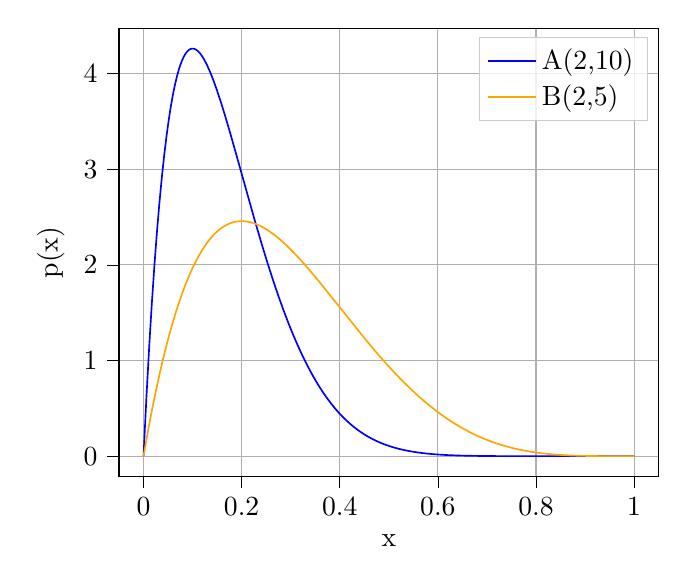
\begin{tikzpicture}

\definecolor{darkgray176}{RGB}{176,176,176}
\definecolor{lightgray204}{RGB}{204,204,204}
\definecolor{orange}{RGB}{255,165,0}

\begin{axis}[
legend cell align={left},
legend style={fill opacity=0.8, draw opacity=1, text opacity=1, draw=lightgray204},
tick align=outside,
tick pos=left,
x grid style={darkgray176},
xlabel={x},
xmajorgrids,
xmin=-0.05, xmax=1.05,
xtick style={color=black},
y grid style={darkgray176},
ylabel={p(x)},
ymajorgrids,
ymin=-0.213081150404745, ymax=4.47470415849965,
ytick style={color=black}
]
\addplot [semithick, blue]
table {%
0 0
0.00600600242614746 0.625795364379883
0.0120120048522949 1.18515026569366
0.0170170068740845 1.60394740104675
0.022022008895874 1.9824925661087
0.0270270109176636 2.32326078414917
0.0320320129394531 2.62860941886902
0.0370370149612427 2.90078258514404
0.0420420169830322 3.14191579818726
0.0470470190048218 3.35403966903687
0.0520520210266113 3.53908467292786
0.056056022644043 3.66885948181152
0.0600600242614746 3.78337502479553
0.0640640258789062 3.88349080085754
0.0680680274963379 3.97003054618835
0.0720720291137695 4.04378366470337
0.0760760307312012 4.10550594329834
0.0790790319442749 4.1443395614624
0.0820820331573486 4.17710781097412
0.0850850343704224 4.20409488677979
0.0880880355834961 4.22557544708252
0.0910910367965698 4.24181604385376
0.0930930376052856 4.24985885620117
0.095095157623291 4.25576162338257
0.0970971584320068 4.25959587097168
0.0980980396270752 4.2607593536377
0.0990991592407227 4.26143217086792
0.100100040435791 4.2616229057312
0.101101160049438 4.26134014129639
0.102102041244507 4.26059198379517
0.103103160858154 4.25938701629639
0.10510516166687 4.25563907623291
0.107107162475586 4.250159740448
0.109109163284302 4.24301290512085
0.112112164497375 4.22929906845093
0.115115165710449 4.21217155456543
0.118118166923523 4.19182348251343
0.122122168540955 4.16000604629517
0.126126170158386 4.12322044372559
0.131131172180176 4.07086420059204
0.136136174201965 4.01211977005005
0.142142176628113 3.93417382240295
0.149149179458618 3.83437347412109
0.157157182693481 3.71061825752258
0.166166186332703 3.56164717674255
0.17717719078064 3.36943769454956
0.193193197250366 3.07829689979553
0.227227210998535 2.45651459693909
0.241241216659546 2.21196222305298
0.253253221511841 2.01144313812256
0.264264225959778 1.8362330198288
0.275275230407715 1.67000436782837
0.285285234451294 1.52709674835205
0.295295238494873 1.39223885536194
0.305305242538452 1.26553130149841
0.314314365386963 1.15846419334412
0.323323249816895 1.0579389333725
0.332332372665405 0.963847637176514
0.341341376304626 0.876042604446411
0.350350379943848 0.794342994689941
0.358358383178711 0.726679801940918
0.366366386413574 0.663517355918884
0.374374389648438 0.604685544967651
0.382382392883301 0.55000627040863
0.390390396118164 0.499295949935913
0.398398399353027 0.452367186546326
0.406406402587891 0.409030914306641
0.414414405822754 0.369097352027893
0.422422409057617 0.332378268241882
0.429429411888123 0.302739262580872
0.436436414718628 0.275295972824097
0.443443417549133 0.249927878379822
0.450450420379639 0.22651731967926
0.457457423210144 0.204949855804443
0.464464426040649 0.18511426448822
0.471471428871155 0.166902899742126
0.47847843170166 0.150212168693542
0.485485553741455 0.134942173957825
0.492492437362671 0.120996952056885
0.499499559402466 0.108285069465637
0.506506443023682 0.0967187881469727
0.513513565063477 0.0862147808074951
0.520520448684692 0.0766938924789429
0.527527570724487 0.0680810213088989
0.534534454345703 0.0603053569793701
0.541541576385498 0.0532996654510498
0.549549579620361 0.0461554527282715
0.557557582855225 0.0398467779159546
0.565565586090088 0.0342921018600464
0.573573589324951 0.0294157266616821
0.582582592964172 0.0246539115905762
0.591591596603394 0.0205715894699097
0.600600600242615 0.0170861482620239
0.610610604286194 0.013823390007019
0.621621608734131 0.0108706951141357
0.633633613586426 0.00828838348388672
0.646646618843079 0.00610864162445068
0.660660743713379 0.00433588027954102
0.676676750183105 0.00287413597106934
0.695695638656616 0.00171232223510742
0.719719648361206 0.000845074653625488
0.751751780509949 0.000296115875244141
0.804804801940918 3.63588333129883e-05
1 0
};
\addlegendentry{A(2,10)}
\addplot [semithick, orange]
table {%
0 0
0.00900900363922119 0.260661602020264
0.0170170068740845 0.476638078689575
0.0250250101089478 0.678374767303467
0.033033013343811 0.866395711898804
0.0410410165786743 1.04121327400208
0.0490490198135376 1.20332884788513
0.0570570230484009 1.35323202610016
0.0650650262832642 1.49140179157257
0.0720720291137695 1.6030433177948
0.0790790319442749 1.70636606216431
0.0860860347747803 1.80167055130005
0.0930930376052856 1.88925051689148
0.100100040435791 1.96939384937286
0.107107162475586 2.04238224029541
0.113113164901733 2.09945774078369
0.119119167327881 2.15164923667908
0.125125169754028 2.19912314414978
0.131131172180176 2.24204325675964
0.137137174606323 2.28057026863098
0.143143177032471 2.31486105918884
0.14814817905426 2.34031200408936
0.15315318107605 2.36301612854004
0.158158183097839 2.38305950164795
0.163163185119629 2.40052652359009
0.167167186737061 2.41270136833191
0.171171188354492 2.42332291603088
0.175175189971924 2.43243193626404
0.179179191589355 2.44006991386414
0.183183193206787 2.44627642631531
0.186186194419861 2.45001602172852
0.189189195632935 2.45298957824707
0.192192196846008 2.45521306991577
0.195195198059082 2.456702709198
0.198198199272156 2.45747470855713
0.201201200485229 2.45754480361938
0.204204201698303 2.45692849159241
0.207207202911377 2.45564103126526
0.210210204124451 2.45369815826416
0.213213205337524 2.45111441612244
0.216216206550598 2.44790530204773
0.22022020816803 2.44267868995667
0.224224209785461 2.4364001750946
0.228228211402893 2.42910432815552
0.233233213424683 2.41860437393188
0.238238215446472 2.40663027763367
0.243243217468262 2.39324569702148
0.249249219894409 2.37540793418884
0.255255222320557 2.35573124885559
0.262262225151062 2.33058547973633
0.269269227981567 2.30323123931885
0.277277231216431 2.26945924758911
0.285285234451294 2.23322010040283
0.294294357299805 2.18976545333862
0.304304361343384 2.1384871006012
0.315315246582031 2.07887697219849
0.327327370643616 2.01056742668152
0.341341376304626 1.92731082439423
0.357357382774353 1.82853019237518
0.378378391265869 1.69493091106415
0.45445442199707 1.20763492584229
0.472472429275513 1.09768640995026
0.488488435745239 1.00322246551514
0.503503561019897 0.917885541915894
0.517517566680908 0.841341972351074
0.531531572341919 0.76801860332489
0.544544458389282 0.702972412109375
0.557557582855225 0.640970587730408
0.56956958770752 0.58651602268219
0.581581592559814 0.534779906272888
0.592592597007751 0.489771127700806
0.603603601455688 0.447086811065674
0.614614605903625 0.406728982925415
0.625625610351562 0.368689060211182
0.635635614395142 0.336103558540344
0.645645618438721 0.305398225784302
0.6556556224823 0.276546955108643
0.665665626525879 0.249517679214478
0.675675630569458 0.224273324012756
0.684684753417969 0.203044891357422
0.6936936378479 0.183194637298584
0.702702760696411 0.164685964584351
0.711711645126343 0.147480130195618
0.720720767974854 0.131535530090332
0.729729652404785 0.116809010505676
0.738738775253296 0.103255271911621
0.747747659683228 0.0908273458480835
0.756756782531738 0.0794768333435059
0.764764785766602 0.0702519416809082
0.772772789001465 0.0618036985397339
0.780780792236328 0.054095983505249
0.789789795875549 0.0462645292282104
0.798798799514771 0.0392718315124512
0.807807803153992 0.0330653190612793
0.816816806793213 0.0275923013687134
0.825825810432434 0.0228005647659302
0.834834814071655 0.0186378955841064
0.844844818115234 0.0146880149841309
0.854854822158813 0.0113821029663086
0.864864826202393 0.00865256786346436
0.875875949859619 0.00623714923858643
0.887887954711914 0.00420808792114258
0.900900840759277 0.00260663032531738
0.915915966033936 0.0013735294342041
0.93293285369873 0.000566244125366211
0.954954981803894 0.000117897987365723
0.99499499797821 0
1 0
};
\addlegendentry{B(2,5)}
\end{axis}

\end{tikzpicture}

\end{figure}

\begin{itemize}
	\item Number of points in grid
	\begin{itemize}
		\item Train: $n\sim \mathcal{U}(5,50)$
		\item Test: Given exact number of points
	\end{itemize}
	\item $S:=\{x_1, \ldots, x_{128}\}$\\ Draw $\{x_1, \ldots, x_n\} \sim \text{UniformSubset}(S, n)$
\end{itemize}

	\begin{itemize}
	\item Draw $\sigma \sim \mathcal{N}(0,0.1)$
	\item Draw noise for each datapoint from $\mathcal{N}(0,\sigma)$
\end{itemize}

\section{Experiments}
\label{exp:experiments}

	\begin{figure}
	\centering
	\resizebox{!}{0.40\textheight}{
		% This file was created with matplot2tikz v0.4.0.
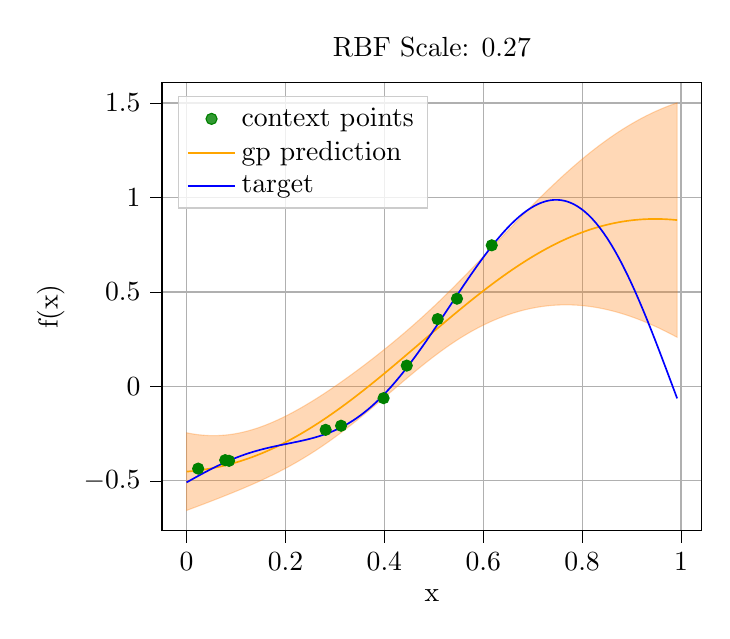
\begin{tikzpicture}

\definecolor{darkgray176}{RGB}{176,176,176}
\definecolor{darkorange25512714}{RGB}{255,127,14}
\definecolor{green}{RGB}{0,128,0}
\definecolor{lightgray204}{RGB}{204,204,204}
\definecolor{orange}{RGB}{255,165,0}

\begin{axis}[
legend cell align={left},
legend style={
  fill opacity=0.8,
  draw opacity=1,
  text opacity=1,
  at={(0.03,0.97)},
  anchor=north west,
  draw=lightgray204
},
tick align=outside,
tick pos=left,
title={RBF Scale: 0.27},
x grid style={darkgray176},
xlabel={x},
xmajorgrids,
xmin=-0.049609375, xmax=1.041796875,
xtick style={color=black},
y grid style={darkgray176},
ylabel={f(x)},
ymajorgrids,
ymin=-0.764390990198043, ymax=1.60873415540691,
ytick style={color=black}
]
\path [draw=darkorange25512714, fill=darkorange25512714, opacity=0.3]
(axis cs:0,-0.245463616773546)
--(axis cs:0,-0.656521665397818)
--(axis cs:0.0078125,-0.648969787345521)
--(axis cs:0.015625,-0.641357306466875)
--(axis cs:0.0234375,-0.63368574994382)
--(axis cs:0.03125,-0.625956021297951)
--(axis cs:0.0390625,-0.618168265902341)
--(axis cs:0.046875,-0.610321734795528)
--(axis cs:0.0546875,-0.602414652145809)
--(axis cs:0.0625,-0.594444092638462)
--(axis cs:0.0703125,-0.586405875687576)
--(axis cs:0.078125,-0.578294483568065)
--(axis cs:0.0859375,-0.570103010207164)
--(axis cs:0.09375,-0.561823146403661)
--(axis cs:0.1015625,-0.553445205666003)
--(axis cs:0.109375,-0.54495819277212)
--(axis cs:0.1171875,-0.536349914731901)
--(axis cs:0.125,-0.527607131317794)
--(axis cs:0.1328125,-0.518715739986708)
--(axis cs:0.140625,-0.509660988097148)
--(axis cs:0.1484375,-0.500427704021322)
--(axis cs:0.15625,-0.491000538167458)
--(axis cs:0.1640625,-0.481364205068657)
--(axis cs:0.171875,-0.471503718477013)
--(axis cs:0.1796875,-0.461404612673858)
--(axis cs:0.1875,-0.451053144782813)
--(axis cs:0.1953125,-0.440436474562818)
--(axis cs:0.203125,-0.42954281979833)
--(axis cs:0.2109375,-0.418361586868234)
--(axis cs:0.21875,-0.406883477285022)
--(axis cs:0.2265625,-0.395100571916639)
--(axis cs:0.234375,-0.383006395236394)
--(axis cs:0.2421875,-0.370595962318183)
--(axis cs:0.25,-0.357865811446516)
--(axis cs:0.2578125,-0.344814025190627)
--(axis cs:0.265625,-0.331440242645226)
--(axis cs:0.2734375,-0.317745665308054)
--(axis cs:0.28125,-0.303733058778389)
--(axis cs:0.2890625,-0.289406752145637)
--(axis cs:0.296875,-0.274772636608218)
--(axis cs:0.3046875,-0.259838164528601)
--(axis cs:0.3125,-0.244612349792445)
--(axis cs:0.3203125,-0.229105769995019)
--(axis cs:0.328125,-0.213330570619701)
--(axis cs:0.3359375,-0.197300470991879)
--(axis cs:0.34375,-0.181030771376391)
--(axis cs:0.3515625,-0.16453836012762)
--(axis cs:0.359375,-0.147841719290765)
--(axis cs:0.3671875,-0.130960926487913)
--(axis cs:0.375,-0.113917650308875)
--(axis cs:0.3828125,-0.0967351357823525)
--(axis cs:0.390625,-0.0794381758625024)
--(axis cs:0.3984375,-0.0620530642859241)
--(axis cs:0.40625,-0.044607524715748)
--(axis cs:0.4140625,-0.0271306109000974)
--(axis cs:0.421875,-0.00965257276066872)
--(axis cs:0.4296875,0.00779531596769478)
--(axis cs:0.4375,0.025180971576287)
--(axis cs:0.4453125,0.0424717566524391)
--(axis cs:0.453125,0.0596347769224114)
--(axis cs:0.4609375,0.0766372133872483)
--(axis cs:0.46875,0.0934466807042754)
--(axis cs:0.4765625,0.110031599072629)
--(axis cs:0.484375,0.126361563791065)
--(axis cs:0.4921875,0.142407694730738)
--(axis cs:0.5,0.158142947678924)
--(axis cs:0.5078125,0.173542371124558)
--(axis cs:0.515625,0.188583295530508)
--(axis cs:0.5234375,0.203245447095345)
--(axis cs:0.53125,0.217510983796849)
--(axis cs:0.5390625,0.231364457334044)
--(axis cs:0.546875,0.244792709670818)
--(axis cs:0.5546875,0.257784716639041)
--(axis cs:0.5625,0.27033139316796)
--(axis cs:0.5703125,0.282425375155786)
--(axis cs:0.578125,0.294060792025957)
--(axis cs:0.5859375,0.305233042008866)
--(axis cs:0.59375,0.315938579606615)
--(axis cs:0.6015625,0.32617472194545)
--(axis cs:0.609375,0.335939478119472)
--(axis cs:0.6171875,0.345231403389611)
--(axis cs:0.625,0.354049478327175)
--(axis cs:0.6328125,0.362393011699704)
--(axis cs:0.640625,0.370261565049039)
--(axis cs:0.6484375,0.377654896435808)
--(axis cs:0.65625,0.384572920637968)
--(axis cs:0.6640625,0.391015683112776)
--(axis cs:0.671875,0.396983345191297)
--(axis cs:0.6796875,0.40247617821551)
--(axis cs:0.6875,0.407494564607628)
--(axis cs:0.6953125,0.412039004149414)
--(axis cs:0.703125,0.416110124026287)
--(axis cs:0.7109375,0.419708691445336)
--(axis cs:0.71875,0.422835627861973)
--(axis cs:0.7265625,0.425492024045201)
--(axis cs:0.734375,0.427679155376855)
--(axis cs:0.7421875,0.429398496917998)
--(axis cs:0.75,0.430651737888901)
--(axis cs:0.7578125,0.43144079530088)
--(axis cs:0.765625,0.431767826552003)
--(axis cs:0.7734375,0.431635240857178)
--(axis cs:0.78125,0.431045709429203)
--(axis cs:0.7890625,0.430002174363149)
--(axis cs:0.796875,0.428507856204094)
--(axis cs:0.8046875,0.42656626019924)
--(axis cs:0.8125,0.424181181251318)
--(axis cs:0.8203125,0.42135670760188)
--(axis cs:0.828125,0.418097223281669)
--(axis cs:0.8359375,0.414407409371304)
--(axis cs:0.84375,0.410292244119685)
--(axis cs:0.8515625,0.405757001970285)
--(axis cs:0.859375,0.400807251547073)
--(axis cs:0.8671875,0.395448852652699)
--(axis cs:0.875,0.389687952331723)
--(axis cs:0.8828125,0.383530980051518)
--(axis cs:0.890625,0.376984642052911)
--(axis cs:0.8984375,0.370055914921896)
--(axis cs:0.90625,0.362752038432877)
--(axis cs:0.9140625,0.355080507712899)
--(axis cs:0.921875,0.34704906477532)
--(axis cs:0.9296875,0.338665689470253)
--(axis cs:0.9375,0.329938589898115)
--(axis cs:0.9453125,0.320876192331425)
--(axis cs:0.953125,0.311487130689041)
--(axis cs:0.9609375,0.301780235605857)
--(axis cs:0.96875,0.29176452313998)
--(axis cs:0.9765625,0.281449183158375)
--(axis cs:0.984375,0.270843567440861)
--(axis cs:0.9921875,0.259957177541405)
--(axis cs:0.9921875,1.50086483060668)
--(axis cs:0.9921875,1.50086483060668)
--(axis cs:0.984375,1.49378672161481)
--(axis cs:0.9765625,1.48627828092629)
--(axis cs:0.96875,1.47833775498946)
--(axis cs:0.9609375,1.46996378923872)
--(axis cs:0.953125,1.4611554366848)
--(axis cs:0.9453125,1.45191216620298)
--(axis cs:0.9375,1.44223387051589)
--(axis cs:0.9296875,1.43212087386868)
--(axis cs:0.921875,1.42157393939636)
--(axis cs:0.9140625,1.41059427618457)
--(axis cs:0.90625,1.39918354602732)
--(axis cs:0.8984375,1.38734386988692)
--(axis cs:0.890625,1.37507783406349)
--(axis cs:0.8828125,1.36238849608386)
--(axis cs:0.875,1.34927939032175)
--(axis cs:0.8671875,1.33575453336357)
--(axis cs:0.859375,1.32181842913672)
--(axis cs:0.8515625,1.30747607381963)
--(axis cs:0.84375,1.29273296055538)
--(axis cs:0.8359375,1.27759508399304)
--(axis cs:0.828125,1.26206894468325)
--(axis cs:0.8203125,1.24616155335654)
--(axis cs:0.8125,1.22988043511461)
--(axis cs:0.8046875,1.21323363356595)
--(axis cs:0.796875,1.1962297149376)
--(axis cs:0.7890625,1.17887777219414)
--(axis cs:0.78125,1.16118742919319)
--(axis cs:0.7734375,1.14316884490261)
--(axis cs:0.765625,1.12483271769844)
--(axis cs:0.7578125,1.10619028975321)
--(axis cs:0.75,1.08725335151067)
--(axis cs:0.7421875,1.06803424622434)
--(axis cs:0.734375,1.04854587451213)
--(axis cs:0.7265625,1.02880169884586)
--(axis cs:0.71875,1.00881574785079)
--(axis cs:0.7109375,0.988602620234382)
--(axis cs:0.703125,0.968177488092129)
--(axis cs:0.6953125,0.947556099248853)
--(axis cs:0.6875,0.926754778183207)
--(axis cs:0.6796875,0.905790424947568)
--(axis cs:0.671875,0.884680511332584)
--(axis cs:0.6640625,0.863443073332829)
--(axis cs:0.65625,0.84209669874664)
--(axis cs:0.6484375,0.820660508491282)
--(axis cs:0.640625,0.799154129939792)
--(axis cs:0.6328125,0.7775976602999)
--(axis cs:0.625,0.756011617778037)
--(axis cs:0.6171875,0.734416878032577)
--(axis cs:0.609375,0.712834593262721)
--(axis cs:0.6015625,0.691286091259701)
--(axis cs:0.59375,0.669792751935384)
--(axis cs:0.5859375,0.648375859320834)
--(axis cs:0.578125,0.627056427876995)
--(axis cs:0.5703125,0.605855003252754)
--(axis cs:0.5625,0.584791439401924)
--(axis cs:0.5546875,0.563884656211629)
--(axis cs:0.546875,0.543152384397029)
--(axis cs:0.5390625,0.52261090717137)
--(axis cs:0.53125,0.502274810784686)
--(axis cs:0.5234375,0.48215675802718)
--(axis cs:0.515625,0.462267299767571)
--(axis cs:0.5078125,0.442614739148324)
--(axis cs:0.5,0.423205060951432)
--(axis cs:0.4921875,0.404041934894077)
--(axis cs:0.484375,0.38512679652759)
--(axis cs:0.4765625,0.366459003588864)
--(axis cs:0.46875,0.348036059863965)
--(axis cs:0.4609375,0.329853893665936)
--(axis cs:0.453125,0.311907174554528)
--(axis cs:0.4453125,0.294189650310489)
--(axis cs:0.4375,0.27669448646339)
--(axis cs:0.4296875,0.259414592597007)
--(axis cs:0.421875,0.242342922745781)
--(axis cs:0.4140625,0.225472740889473)
--(axis cs:0.40625,0.208797846319522)
--(axis cs:0.3984375,0.192312757072031)
--(axis cs:0.390625,0.176012852430631)
--(axis cs:0.3828125,0.159894477579337)
--(axis cs:0.375,0.143955014833442)
--(axis cs:0.3671875,0.12819292658027)
--(axis cs:0.359375,0.112607775248498)
--(axis cs:0.3515625,0.0972002254337523)
--(axis cs:0.34375,0.0819720328681524)
--(axis cs:0.3359375,0.0669260243395844)
--(axis cs:0.328125,0.0520660720241412)
--(axis cs:0.3203125,0.037397065048796)
--(axis cs:0.3125,0.022924880485652)
--(axis cs:0.3046875,0.0086563554121587)
--(axis cs:0.296875,-0.0054007388411354)
--(axis cs:0.2890625,-0.0192377195949132)
--(axis cs:0.28125,-0.0328450126346484)
--(axis cs:0.2734375,-0.0462121690742715)
--(axis cs:0.265625,-0.0593278797716453)
--(axis cs:0.2578125,-0.0721799881446169)
--(axis cs:0.25,-0.0847555025768614)
--(axis cs:0.2421875,-0.0970406099394468)
--(axis cs:0.234375,-0.109020692085459)
--(axis cs:0.2265625,-0.120680347492559)
--(axis cs:0.21875,-0.13200342051674)
--(axis cs:0.2109375,-0.14297304095551)
--(axis cs:0.203125,-0.153571676767881)
--(axis cs:0.1953125,-0.163781202821176)
--(axis cs:0.1875,-0.173582988384893)
--(axis cs:0.1796875,-0.182958005722401)
--(axis cs:0.171875,-0.191886961500601)
--(axis cs:0.1640625,-0.2003504518192)
--(axis cs:0.15625,-0.208329140453493)
--(axis cs:0.1484375,-0.215803958442461)
--(axis cs:0.140625,-0.22275632151615)
--(axis cs:0.1328125,-0.229168360167916)
--(axis cs:0.125,-0.235023155603417)
--(axis cs:0.1171875,-0.240304973528026)
--(axis cs:0.109375,-0.244999486953931)
--(axis cs:0.1015625,-0.249093979068916)
--(axis cs:0.09375,-0.25257751779508)
--(axis cs:0.0859375,-0.25544109497167)
--(axis cs:0.078125,-0.257677725017003)
--(axis cs:0.0703125,-0.259282500268301)
--(axis cs:0.0625,-0.260252602715121)
--(axis cs:0.0546875,-0.260587274265309)
--(axis cs:0.046875,-0.260287749771927)
--(axis cs:0.0390625,-0.259357158627849)
--(axis cs:0.03125,-0.257800401706798)
--(axis cs:0.0234375,-0.255624010786819)
--(axis cs:0.015625,-0.252835997399073)
--(axis cs:0.0078125,-0.249445697416571)
--(axis cs:0,-0.245463616773546)
--cycle;

\addplot [draw=green, fill=green, mark=*, only marks]
table{%
x  y
0.0234375 -0.435152769088745
0.078125 -0.390416473150253
0.0859375 -0.39392226934433
0.28125 -0.229927331209183
0.3125 -0.208194002509117
0.3984375 -0.0621931217610836
0.4453125 0.110128581523895
0.5078125 0.356279462575912
0.546875 0.46435934305191
0.6171875 0.746831953525543
};
\addlegendentry{context points}
\addplot [semithick, orange]
table {%
0 -0.450992641085682
0.0078125 -0.449207742381046
0.015625 -0.447096651932974
0.0234375 -0.444654880365319
0.03125 -0.441878211502374
0.0390625 -0.438762712265095
0.046875 -0.435304742283728
0.0546875 -0.431500963205559
0.0625 -0.427348347676792
0.0703125 -0.422844187977939
0.078125 -0.417986104292534
0.0859375 -0.412772052589417
0.09375 -0.40720033209937
0.1015625 -0.401269592367459
0.109375 -0.394978839863025
0.1171875 -0.388327444129963
0.125 -0.381315143460606
0.1328125 -0.373942050077312
0.140625 -0.366208654806649
0.1484375 -0.358115831231892
0.15625 -0.349664839310475
0.1640625 -0.340857328443928
0.171875 -0.331695339988807
0.1796875 -0.322181309198129
0.1875 -0.312318066583853
0.1953125 -0.302108838691997
0.203125 -0.291557248283106
0.2109375 -0.280667313911872
0.21875 -0.269443448900881
0.2265625 -0.257890459704599
0.234375 -0.246013543660927
0.2421875 -0.233818286128815
0.25 -0.221310657011689
0.2578125 -0.208497006667622
0.265625 -0.195384061208436
0.2734375 -0.181978917191163
0.28125 -0.168289035706519
0.2890625 -0.154322235870275
0.296875 -0.140086687724677
0.3046875 -0.125590904558221
0.3125 -0.110843734653396
0.3203125 -0.0958543524731112
0.328125 -0.0806322492977798
0.3359375 -0.0651872233261472
0.34375 -0.0495293692541194
0.3515625 -0.033669067346934
0.359375 -0.0176169720211337
0.3671875 -0.00138399995382166
0.375 0.0150186822622835
0.3828125 0.0315796708984921
0.390625 0.0482873382840641
0.3984375 0.0651298463930532
0.40625 0.0820951608018872
0.4140625 0.099171064994688
0.421875 0.116345174992556
0.4296875 0.133604954282351
0.4375 0.150937729019839
0.4453125 0.168330703481464
0.453125 0.18577097573847
0.4609375 0.203245553526592
0.46875 0.22074137028412
0.4765625 0.238245301330746
0.484375 0.255744180159328
0.4921875 0.273224814812407
0.5 0.290674004315178
0.5078125 0.308078555136441
0.515625 0.32542529764904
0.5234375 0.342701102561263
0.53125 0.359892897290767
0.5390625 0.376987682252707
0.546875 0.393972547033924
0.5546875 0.410834686425335
0.5625 0.427561416284942
0.5703125 0.44414018920427
0.578125 0.460558609951476
0.5859375 0.47680445066485
0.59375 0.492865665770999
0.6015625 0.508730406602576
0.609375 0.524387035691096
0.6171875 0.539824140711094
0.625 0.555030548052606
0.6328125 0.569995335999802
0.640625 0.584707847494415
0.6484375 0.599157702463545
0.65625 0.613334809692304
0.6640625 0.627229378222802
0.671875 0.64083192826194
0.6796875 0.654133301581539
0.6875 0.667124671395418
0.6953125 0.679797551699133
0.703125 0.692143806059208
0.7109375 0.704155655839859
0.71875 0.71582568785638
0.7265625 0.727146861445529
0.734375 0.738112514944491
0.7421875 0.748716371571168
0.75 0.758952544699787
0.7578125 0.768815542527047
0.765625 0.778300272125222
0.7734375 0.787402042879894
0.78125 0.796116569311196
0.7890625 0.804439973278643
0.796875 0.812368785570846
0.8046875 0.819899946882597
0.8125 0.827030808182964
0.8203125 0.83375913047921
0.828125 0.840083083982458
0.8359375 0.84600124668217
0.84375 0.851512602337531
0.8515625 0.856616537894956
0.859375 0.861312840341896
0.8671875 0.865601693008134
0.875 0.869483671326735
0.8828125 0.872959738067687
0.890625 0.876031238058199
0.8984375 0.878699892404409
0.90625 0.880967792230101
0.9140625 0.882837391948734
0.921875 0.884311502085841
0.9296875 0.885393281669469
0.9375 0.886086230207001
0.9453125 0.886394179267202
0.953125 0.886321283686921
0.9609375 0.885872012422291
0.96875 0.885051139064719
0.9765625 0.883863732042332
0.984375 0.882315144527836
0.9921875 0.880411004074045
};
\addlegendentry{gp prediction}
\addplot [semithick, blue]
table {%
0 -0.50814962387085
0.0078125 -0.496681034564972
0.015625 -0.485288977622986
0.0234375 -0.474015474319458
0.03125 -0.46290135383606
0.0390625 -0.451987385749817
0.046875 -0.441312849521637
0.0546875 -0.430915027856827
0.0625 -0.420828431844711
0.0703125 -0.411084443330765
0.078125 -0.401710242033005
0.0859375 -0.392728626728058
0.09375 -0.384157747030258
0.1015625 -0.376009970903397
0.109375 -0.368293344974518
0.1171875 -0.361008644104004
0.125 -0.354151487350464
0.1328125 -0.347710967063904
0.140625 -0.341671019792557
0.1484375 -0.336008131504059
0.15625 -0.330694168806076
0.1640625 -0.32569432258606
0.171875 -0.32096928358078
0.1796875 -0.316473960876465
0.1875 -0.312158674001694
0.1953125 -0.3079694211483
0.203125 -0.303848713636398
0.2109375 -0.299735546112061
0.21875 -0.29556605219841
0.2265625 -0.291274398565292
0.234375 -0.286793500185013
0.2421875 -0.282055079936981
0.25 -0.27699014544487
0.2578125 -0.271531194448471
0.265625 -0.265610426664352
0.2734375 -0.259162724018097
0.28125 -0.252124667167664
0.2890625 -0.244435146450996
0.296875 -0.236037015914917
0.3046875 -0.226876229047775
0.3125 -0.216903626918793
0.3203125 -0.206074655056
0.328125 -0.194348722696304
0.3359375 -0.18169204890728
0.34375 -0.168075278401375
0.3515625 -0.153475224971771
0.359375 -0.137874752283096
0.3671875 -0.121262766420841
0.375 -0.103634275496006
0.3828125 -0.084990382194519
0.390625 -0.0653383731842041
0.3984375 -0.0446914620697498
0.40625 -0.0230690203607082
0.4140625 -0.000495294865686446
0.421875 0.0229989755898714
0.4296875 0.0473779588937759
0.4375 0.0726012885570526
0.4453125 0.0986236706376076
0.453125 0.125395134091377
0.4609375 0.152861669659615
0.46875 0.180965840816498
0.4765625 0.209646478295326
0.484375 0.238839074969292
0.4921875 0.268476754426956
0.5 0.298489660024643
0.5078125 0.328806608915329
0.515625 0.359353482723236
0.5234375 0.390055239200592
0.53125 0.420835047960281
0.5390625 0.451615005731583
0.546875 0.482316374778748
0.5546875 0.512859582901001
0.5625 0.543164312839508
0.5703125 0.573149740695953
0.578125 0.602734863758087
0.5859375 0.631838083267212
0.59375 0.660378038883209
0.6015625 0.688272356987
0.609375 0.715439200401306
0.6171875 0.741796851158142
0.625 0.767262697219849
0.6328125 0.791754961013794
0.640625 0.815191507339478
0.6484375 0.837490320205688
0.65625 0.858569502830505
0.6640625 0.878347873687744
0.671875 0.8967444896698
0.6796875 0.913678407669067
0.6875 0.929070115089417
0.6953125 0.942841053009033
0.703125 0.954913258552551
0.7109375 0.965210914611816
0.71875 0.973659873008728
0.7265625 0.980187714099884
0.734375 0.984725594520569
0.7421875 0.987206816673279
0.75 0.987568557262421
0.7578125 0.98575222492218
0.765625 0.981703698635101
0.7734375 0.975374042987823
0.78125 0.966719806194305
0.7890625 0.95570433139801
0.796875 0.942297518253326
0.8046875 0.926477015018463
0.8125 0.908228397369385
0.8203125 0.887546002864838
0.828125 0.864433288574219
0.8359375 0.838903546333313
0.84375 0.810979902744293
0.8515625 0.780696392059326
0.859375 0.748097896575928
0.8671875 0.713239848613739
0.875 0.676189780235291
0.8828125 0.637026131153107
0.890625 0.595839262008667
0.8984375 0.552730083465576
0.90625 0.507811665534973
0.9140625 0.461207449436188
0.921875 0.413051575422287
0.9296875 0.363487958908081
0.9375 0.312670201063156
0.9453125 0.260761171579361
0.953125 0.207931026816368
0.9609375 0.154357388615608
0.96875 0.100224360823631
0.9765625 0.0457205921411514
0.984375 -0.00896052457392216
0.9921875 -0.0636230930685997
};
\addlegendentry{target}
\end{axis}

\end{tikzpicture}

		% This file was created with matplot2tikz v0.4.0.
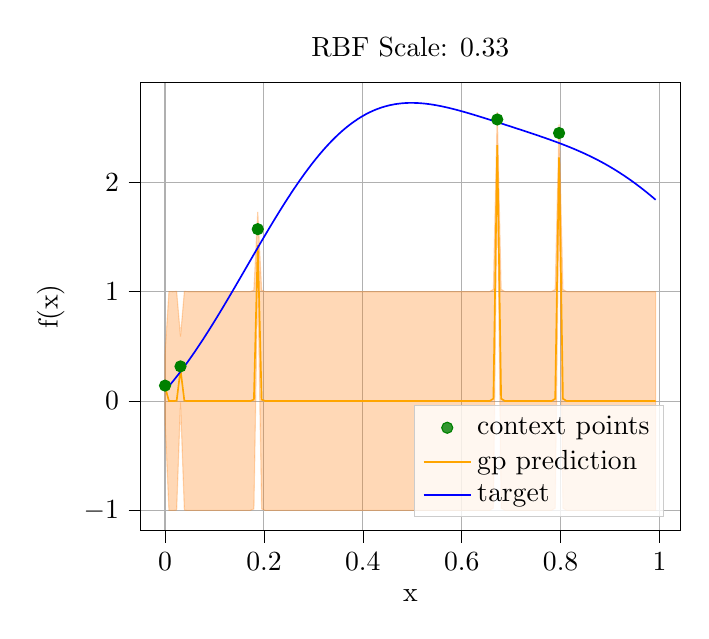
\begin{tikzpicture}

\definecolor{darkgray176}{RGB}{176,176,176}
\definecolor{darkorange25512714}{RGB}{255,127,14}
\definecolor{green}{RGB}{0,128,0}
\definecolor{lightgray204}{RGB}{204,204,204}
\definecolor{orange}{RGB}{255,165,0}

\begin{axis}[
legend pos={south east},
legend cell align={left},
legend style={
  fill opacity=0.8,
  draw opacity=1,
  text opacity=1,
  draw=lightgray204
},
tick align=outside,
tick pos=left,
title={RBF Scale: 0.33},
x grid style={darkgray176},
xlabel={x},
xmajorgrids,
xmin=-0.049609375, xmax=1.041796875,
xtick style={color=black},
y grid style={darkgray176},
ylabel={f(x)},
ymajorgrids,
ymin=-1.1863420009613, ymax=2.91318202018738,
ytick style={color=black}
]
\path [draw=darkorange25512714, fill=darkorange25512714, opacity=0.3]
(axis cs:0,0.430150508973854)
--(axis cs:0,-0.172872180181674)
--(axis cs:0.0078125,-0.998748464321721)
--(axis cs:0.015625,-0.999999996722257)
--(axis cs:0.0234375,-0.997244417904979)
--(axis cs:0.03125,-0.0131351733015166)
--(axis cs:0.0390625,-0.997244417904979)
--(axis cs:0.046875,-0.999999997733362)
--(axis cs:0.0546875,-1)
--(axis cs:0.0625,-1)
--(axis cs:0.0703125,-1)
--(axis cs:0.078125,-1)
--(axis cs:0.0859375,-1)
--(axis cs:0.09375,-1)
--(axis cs:0.1015625,-1)
--(axis cs:0.109375,-1)
--(axis cs:0.1171875,-1)
--(axis cs:0.125,-1)
--(axis cs:0.1328125,-1)
--(axis cs:0.140625,-1)
--(axis cs:0.1484375,-1)
--(axis cs:0.15625,-1)
--(axis cs:0.1640625,-1)
--(axis cs:0.171875,-0.999999988766446)
--(axis cs:0.1796875,-0.986502644021871)
--(axis cs:0.1875,1.12769318782551)
--(axis cs:0.1953125,-0.986502644021871)
--(axis cs:0.203125,-0.999999988766446)
--(axis cs:0.2109375,-1)
--(axis cs:0.21875,-1)
--(axis cs:0.2265625,-1)
--(axis cs:0.234375,-1)
--(axis cs:0.2421875,-1)
--(axis cs:0.25,-1)
--(axis cs:0.2578125,-1)
--(axis cs:0.265625,-1)
--(axis cs:0.2734375,-1)
--(axis cs:0.28125,-1)
--(axis cs:0.2890625,-1)
--(axis cs:0.296875,-1)
--(axis cs:0.3046875,-1)
--(axis cs:0.3125,-1)
--(axis cs:0.3203125,-1)
--(axis cs:0.328125,-1)
--(axis cs:0.3359375,-1)
--(axis cs:0.34375,-1)
--(axis cs:0.3515625,-1)
--(axis cs:0.359375,-1)
--(axis cs:0.3671875,-1)
--(axis cs:0.375,-1)
--(axis cs:0.3828125,-1)
--(axis cs:0.390625,-1)
--(axis cs:0.3984375,-1)
--(axis cs:0.40625,-1)
--(axis cs:0.4140625,-1)
--(axis cs:0.421875,-1)
--(axis cs:0.4296875,-1)
--(axis cs:0.4375,-1)
--(axis cs:0.4453125,-1)
--(axis cs:0.453125,-1)
--(axis cs:0.4609375,-1)
--(axis cs:0.46875,-1)
--(axis cs:0.4765625,-1)
--(axis cs:0.484375,-1)
--(axis cs:0.4921875,-1)
--(axis cs:0.5,-1)
--(axis cs:0.5078125,-1)
--(axis cs:0.515625,-1)
--(axis cs:0.5234375,-1)
--(axis cs:0.53125,-1)
--(axis cs:0.5390625,-1)
--(axis cs:0.546875,-1)
--(axis cs:0.5546875,-1)
--(axis cs:0.5625,-1)
--(axis cs:0.5703125,-1)
--(axis cs:0.578125,-1)
--(axis cs:0.5859375,-1)
--(axis cs:0.59375,-1)
--(axis cs:0.6015625,-1)
--(axis cs:0.609375,-1)
--(axis cs:0.6171875,-1)
--(axis cs:0.625,-1)
--(axis cs:0.6328125,-1)
--(axis cs:0.640625,-1)
--(axis cs:0.6484375,-1)
--(axis cs:0.65625,-0.999999981600401)
--(axis cs:0.6640625,-0.977918195325254)
--(axis cs:0.671875,2.03940317579518)
--(axis cs:0.6796875,-0.977918195325254)
--(axis cs:0.6875,-0.999999981600401)
--(axis cs:0.6953125,-1)
--(axis cs:0.703125,-1)
--(axis cs:0.7109375,-1)
--(axis cs:0.71875,-1)
--(axis cs:0.7265625,-1)
--(axis cs:0.734375,-1)
--(axis cs:0.7421875,-1)
--(axis cs:0.75,-1)
--(axis cs:0.7578125,-1)
--(axis cs:0.765625,-1)
--(axis cs:0.7734375,-1)
--(axis cs:0.78125,-0.999999982487233)
--(axis cs:0.7890625,-0.978980560592891)
--(axis cs:0.796875,1.92657484405172)
--(axis cs:0.8046875,-0.978980560592891)
--(axis cs:0.8125,-0.999999982487233)
--(axis cs:0.8203125,-1)
--(axis cs:0.828125,-1)
--(axis cs:0.8359375,-1)
--(axis cs:0.84375,-1)
--(axis cs:0.8515625,-1)
--(axis cs:0.859375,-1)
--(axis cs:0.8671875,-1)
--(axis cs:0.875,-1)
--(axis cs:0.8828125,-1)
--(axis cs:0.890625,-1)
--(axis cs:0.8984375,-1)
--(axis cs:0.90625,-1)
--(axis cs:0.9140625,-1)
--(axis cs:0.921875,-1)
--(axis cs:0.9296875,-1)
--(axis cs:0.9375,-1)
--(axis cs:0.9453125,-1)
--(axis cs:0.953125,-1)
--(axis cs:0.9609375,-1)
--(axis cs:0.96875,-1)
--(axis cs:0.9765625,-1)
--(axis cs:0.984375,-1)
--(axis cs:0.9921875,-1)
--(axis cs:0.9921875,1)
--(axis cs:0.9921875,1)
--(axis cs:0.984375,1)
--(axis cs:0.9765625,1)
--(axis cs:0.96875,1)
--(axis cs:0.9609375,1)
--(axis cs:0.953125,1)
--(axis cs:0.9453125,1)
--(axis cs:0.9375,1)
--(axis cs:0.9296875,1)
--(axis cs:0.921875,1)
--(axis cs:0.9140625,1)
--(axis cs:0.90625,1)
--(axis cs:0.8984375,1)
--(axis cs:0.890625,1)
--(axis cs:0.8828125,1)
--(axis cs:0.875,1)
--(axis cs:0.8671875,1)
--(axis cs:0.859375,1)
--(axis cs:0.8515625,1)
--(axis cs:0.84375,1)
--(axis cs:0.8359375,1)
--(axis cs:0.828125,1)
--(axis cs:0.8203125,1)
--(axis cs:0.8125,1.00000001751277)
--(axis cs:0.8046875,1.02093884081427)
--(axis cs:0.796875,2.52959753320725)
--(axis cs:0.7890625,1.02093884081427)
--(axis cs:0.78125,1.00000001751277)
--(axis cs:0.7734375,1)
--(axis cs:0.765625,1)
--(axis cs:0.7578125,1)
--(axis cs:0.75,1)
--(axis cs:0.7421875,1)
--(axis cs:0.734375,1)
--(axis cs:0.7265625,1)
--(axis cs:0.71875,1)
--(axis cs:0.7109375,1)
--(axis cs:0.703125,1)
--(axis cs:0.6953125,1)
--(axis cs:0.6875,1.0000000183996)
--(axis cs:0.6796875,1.02200120608191)
--(axis cs:0.671875,2.64242586495071)
--(axis cs:0.6640625,1.02200120608191)
--(axis cs:0.65625,1.0000000183996)
--(axis cs:0.6484375,1)
--(axis cs:0.640625,1)
--(axis cs:0.6328125,1)
--(axis cs:0.625,1)
--(axis cs:0.6171875,1)
--(axis cs:0.609375,1)
--(axis cs:0.6015625,1)
--(axis cs:0.59375,1)
--(axis cs:0.5859375,1)
--(axis cs:0.578125,1)
--(axis cs:0.5703125,1)
--(axis cs:0.5625,1)
--(axis cs:0.5546875,1)
--(axis cs:0.546875,1)
--(axis cs:0.5390625,1)
--(axis cs:0.53125,1)
--(axis cs:0.5234375,1)
--(axis cs:0.515625,1)
--(axis cs:0.5078125,1)
--(axis cs:0.5,1)
--(axis cs:0.4921875,1)
--(axis cs:0.484375,1)
--(axis cs:0.4765625,1)
--(axis cs:0.46875,1)
--(axis cs:0.4609375,1)
--(axis cs:0.453125,1)
--(axis cs:0.4453125,1)
--(axis cs:0.4375,1)
--(axis cs:0.4296875,1)
--(axis cs:0.421875,1)
--(axis cs:0.4140625,1)
--(axis cs:0.40625,1)
--(axis cs:0.3984375,1)
--(axis cs:0.390625,1)
--(axis cs:0.3828125,1)
--(axis cs:0.375,1)
--(axis cs:0.3671875,1)
--(axis cs:0.359375,1)
--(axis cs:0.3515625,1)
--(axis cs:0.34375,1)
--(axis cs:0.3359375,1)
--(axis cs:0.328125,1)
--(axis cs:0.3203125,1)
--(axis cs:0.3125,1)
--(axis cs:0.3046875,1)
--(axis cs:0.296875,1)
--(axis cs:0.2890625,1)
--(axis cs:0.28125,1)
--(axis cs:0.2734375,1)
--(axis cs:0.265625,1)
--(axis cs:0.2578125,1)
--(axis cs:0.25,1)
--(axis cs:0.2421875,1)
--(axis cs:0.234375,1)
--(axis cs:0.2265625,1)
--(axis cs:0.21875,1)
--(axis cs:0.2109375,1)
--(axis cs:0.203125,1.00000001123355)
--(axis cs:0.1953125,1.01341675738529)
--(axis cs:0.1875,1.73071587698104)
--(axis cs:0.1796875,1.01341675738529)
--(axis cs:0.171875,1.00000001123355)
--(axis cs:0.1640625,1)
--(axis cs:0.15625,1)
--(axis cs:0.1484375,1)
--(axis cs:0.140625,1)
--(axis cs:0.1328125,1)
--(axis cs:0.125,1)
--(axis cs:0.1171875,1)
--(axis cs:0.109375,1)
--(axis cs:0.1015625,1)
--(axis cs:0.09375,1)
--(axis cs:0.0859375,1)
--(axis cs:0.078125,1)
--(axis cs:0.0703125,1)
--(axis cs:0.0625,1)
--(axis cs:0.0546875,1)
--(axis cs:0.046875,1.00000000226664)
--(axis cs:0.0390625,1.00267498350218)
--(axis cs:0.03125,0.589887515854011)
--(axis cs:0.0234375,1.00267498350218)
--(axis cs:0.015625,1.00000000327774)
--(axis cs:0.0078125,1.00117093708544)
--(axis cs:0,0.430150508973854)
--cycle;

\addplot [draw=green, fill=green, mark=*, only marks]
table{%
x  y
0 0.14150308072567
0.03125 0.317213773727417
0.1875 1.57212495803833
0.671875 2.57500600814819
0.796875 2.45089483261108
};
\addlegendentry{context points}
\addplot [semithick, orange]
table {%
0 0.12863916439609
0.0078125 0.00121123638185998
0.015625 3.27774236090191e-09
0.0234375 0.00271528279860228
0.03125 0.288376171276247
0.0390625 0.00271528279860228
0.046875 2.26663796654603e-09
0.0546875 1.67749271731144e-19
0.0625 1.10065325315756e-33
0.0703125 6.40253252647661e-52
0.078125 3.30190412754361e-74
0.0859375 1.50969257322636e-100
0.09375 6.1196131866807e-131
0.1015625 2.19923084869799e-165
0.109375 4.17336952429216e-203
0.1171875 1.08994813366508e-164
0.125 3.03290624334581e-130
0.1328125 7.48210040601367e-100
0.140625 1.63643768615189e-73
0.1484375 3.17312226776675e-51
0.15625 5.45488419190608e-33
0.1640625 8.31372503506265e-19
0.171875 1.1233553870863e-08
0.1796875 0.0134570566817099
0.1875 1.42920453240328
0.1953125 0.0134570566817105
0.203125 1.1233553870863e-08
0.2109375 8.31372503506371e-19
0.21875 5.45488419190608e-33
0.2265625 3.17312226776711e-51
0.234375 1.63643768615189e-73
0.2421875 7.48210040601473e-100
0.25 3.03290624334581e-130
0.2578125 1.08994813366527e-164
0.265625 3.47267445816914e-203
0.2734375 9.80920266070464e-246
0.28125 2.45648850094303e-292
0.2890625 0
0.296875 0
0.3046875 0
0.3125 0
0.3203125 0
0.328125 0
0.3359375 0
0.34375 0
0.3515625 0
0.359375 0
0.3671875 0
0.375 0
0.3828125 0
0.390625 0
0.3984375 0
0.40625 0
0.4140625 0
0.421875 0
0.4296875 0
0.4375 0
0.4453125 0
0.453125 0
0.4609375 0
0.46875 0
0.4765625 0
0.484375 0
0.4921875 0
0.5 0
0.5078125 0
0.515625 0
0.5234375 0
0.53125 0
0.5390625 0
0.546875 0
0.5546875 0
0.5625 0
0.5703125 0
0.578125 4.02351760760029e-292
0.5859375 1.60666331662914e-245
0.59375 5.68794310356012e-203
0.6015625 1.7852416184694e-164
0.609375 4.96764046223626e-130
0.6171875 1.22550391397626e-99
0.625 2.6803446633057e-73
0.6328125 5.19730229167814e-51
0.640625 8.93463274309199e-33
0.6484375 1.36171689997672e-18
0.65625 1.83995983608262e-08
0.6640625 0.0220415053783273
0.671875 2.34091452037295
0.6796875 0.0220415053783273
0.6875 1.83995983608262e-08
0.6953125 1.36171689997637e-18
0.703125 8.93463274308894e-33
0.7109375 5.19730229167364e-51
0.71875 2.6803446633057e-73
0.7265625 1.22550391397626e-99
0.734375 9.69584860809468e-130
0.7421875 1.16643658752942e-99
0.75 2.55115634214902e-73
0.7578125 4.9468006428426e-51
0.765625 8.50399775050121e-33
0.7734375 1.29608432570145e-18
0.78125 1.75127671802195e-08
0.7890625 0.0209791401106904
0.796875 2.22808618862949
0.8046875 0.0209791401106904
0.8125 1.75127671802195e-08
0.8203125 1.29608432570078e-18
0.828125 8.50399775049528e-33
0.8359375 4.94680064283831e-51
0.84375 2.55115634214902e-73
0.8515625 1.16643658752942e-99
0.859375 4.72820814585842e-130
0.8671875 1.69919583088466e-164
0.875 5.41379335317327e-203
0.8828125 1.52922471726368e-245
0.890625 3.82959050113644e-292
0.8984375 0
0.90625 0
0.9140625 0
0.921875 0
0.9296875 0
0.9375 0
0.9453125 0
0.953125 0
0.9609375 0
0.96875 0
0.9765625 0
0.984375 0
0.9921875 0
};
\addlegendentry{gp prediction}
\addplot [semithick, blue]
table {%
0 0.0955265462398529
0.0078125 0.136524334549904
0.015625 0.179150179028511
0.0234375 0.223369240760803
0.03125 0.269141018390656
0.0390625 0.316419631242752
0.046875 0.36515349149704
0.0546875 0.415285497903824
0.0625 0.466753244400024
0.0703125 0.51948881149292
0.078125 0.573419392108917
0.0859375 0.628467321395874
0.09375 0.684549629688263
0.1015625 0.741579234600067
0.109375 0.79946506023407
0.1171875 0.858110666275024
0.125 0.917417705059052
0.1328125 0.977283418178558
0.140625 1.03760206699371
0.1484375 1.0982654094696
0.15625 1.15916299819946
0.1640625 1.2201828956604
0.171875 1.28121089935303
0.1796875 1.34213268756866
0.1875 1.4028332233429
0.1953125 1.46319723129272
0.203125 1.52311062812805
0.2109375 1.58245944976807
0.21875 1.64113187789917
0.2265625 1.69901752471924
0.234375 1.75600910186768
0.2421875 1.81200134754181
0.25 1.86689341068268
0.2578125 1.92058742046356
0.265625 1.97299003601074
0.2734375 2.02401280403137
0.28125 2.0735719203949
0.2890625 2.12158966064453
0.296875 2.16799283027649
0.3046875 2.21271586418152
0.3125 2.25569772720337
0.3203125 2.29688572883606
0.328125 2.33623242378235
0.3359375 2.37369799613953
0.34375 2.4092493057251
0.3515625 2.44286036491394
0.359375 2.47451233863831
0.3671875 2.50419330596924
0.375 2.53189849853516
0.3828125 2.55762982368469
0.390625 2.58139657974243
0.3984375 2.60321354866028
0.40625 2.62310338020325
0.4140625 2.64109349250793
0.421875 2.65721845626831
0.4296875 2.67151689529419
0.4375 2.68403458595276
0.4453125 2.69482064247131
0.453125 2.70392894744873
0.4609375 2.71141815185547
0.46875 2.71734976768494
0.4765625 2.72178888320923
0.484375 2.72480320930481
0.4921875 2.72646284103394
0.5 2.72684001922607
0.5078125 2.72600746154785
0.515625 2.72403955459595
0.5234375 2.72101068496704
0.53125 2.71699547767639
0.5390625 2.71206784248352
0.546875 2.70630121231079
0.5546875 2.69976735115051
0.5625 2.69253611564636
0.5703125 2.68467569351196
0.578125 2.67625164985657
0.5859375 2.66732668876648
0.59375 2.65796041488647
0.6015625 2.64820957183838
0.609375 2.63812637329102
0.6171875 2.62775993347168
0.625 2.61715507507324
0.6328125 2.60635256767273
0.640625 2.59538865089417
0.6484375 2.58429551124573
0.65625 2.57310009002686
0.6640625 2.56182622909546
0.671875 2.55049157142639
0.6796875 2.5391104221344
0.6875 2.52769207954407
0.6953125 2.51624178886414
0.703125 2.50476026535034
0.7109375 2.49324369430542
0.71875 2.48168587684631
0.7265625 2.47007441520691
0.734375 2.45839500427246
0.7421875 2.44662928581238
0.75 2.43475580215454
0.7578125 2.42275023460388
0.765625 2.41058540344238
0.7734375 2.39823174476624
0.78125 2.385657787323
0.7890625 2.37282967567444
0.796875 2.35971236228943
0.8046875 2.34627032279968
0.8125 2.33246564865112
0.8203125 2.31826090812683
0.828125 2.30361795425415
0.8359375 2.288498878479
0.84375 2.27286553382874
0.8515625 2.2566819190979
0.859375 2.23991131782532
0.8671875 2.2225193977356
0.875 2.20447278022766
0.8828125 2.18574047088623
0.890625 2.16629314422607
0.8984375 2.14610457420349
0.90625 2.12515044212341
0.9140625 2.10340976715088
0.921875 2.08086442947388
0.9296875 2.05750036239624
0.9375 2.03330636024475
0.9453125 2.00827503204346
0.953125 1.98240351676941
0.9609375 1.9556919336319
0.96875 1.92814552783966
0.9765625 1.899773478508
0.984375 1.87058913707733
0.9921875 1.84061014652252
};
\addlegendentry{target}
\end{axis}

\end{tikzpicture}

	}
	\resizebox{!}{0.40\textheight}{
		% This file was created with matplot2tikz v0.4.0.
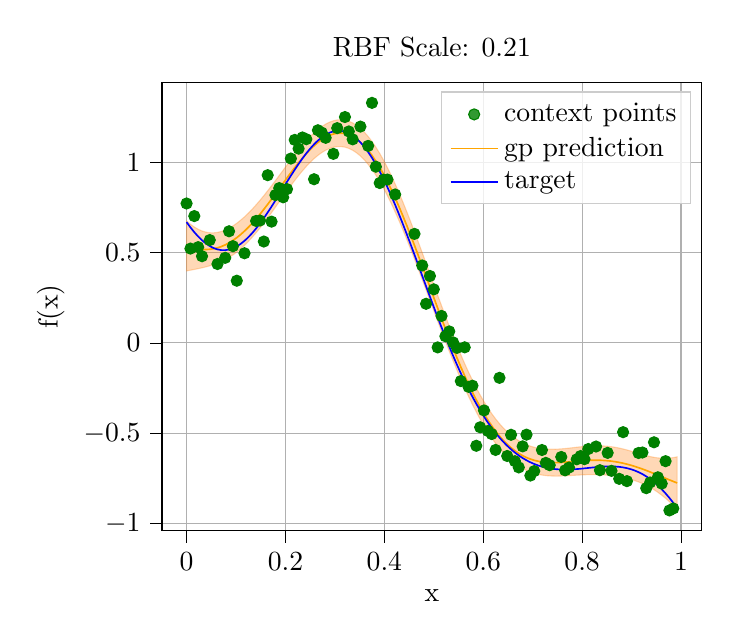
\begin{tikzpicture}

\definecolor{darkgray176}{RGB}{176,176,176}
\definecolor{darkorange25512714}{RGB}{255,127,14}
\definecolor{green}{RGB}{0,128,0}
\definecolor{lightgray204}{RGB}{204,204,204}
\definecolor{orange}{RGB}{255,165,0}

\begin{axis}[
legend cell align={left},
legend style={fill opacity=0.8, draw opacity=1, text opacity=1, draw=lightgray204},
tick align=outside,
tick pos=left,
title={RBF Scale: 0.21},
x grid style={darkgray176},
xlabel={x},
xmajorgrids,
xmin=-0.049609375, xmax=1.041796875,
xtick style={color=black},
y grid style={darkgray176},
ylabel={f(x)},
ymajorgrids,
ymin=-1.03975863456726, ymax=1.44098014831543,
ytick style={color=black}
]
\path [draw=darkorange25512714, fill=darkorange25512714, opacity=0.3]
(axis cs:0,0.674425466042734)
--(axis cs:0,0.398245043076177)
--(axis cs:0.0078125,0.402341016518767)
--(axis cs:0.015625,0.40650681290413)
--(axis cs:0.0234375,0.410860250838664)
--(axis cs:0.03125,0.41553690032933)
--(axis cs:0.0390625,0.420694940013351)
--(axis cs:0.046875,0.426516902954857)
--(axis cs:0.0546875,0.433206272460823)
--(axis cs:0.0625,0.44097827024004)
--(axis cs:0.0703125,0.450046224461232)
--(axis cs:0.078125,0.460606462529595)
--(axis cs:0.0859375,0.472824864506443)
--(axis cs:0.09375,0.486827145078188)
--(axis cs:0.1015625,0.50269344200463)
--(axis cs:0.109375,0.520456659983196)
--(axis cs:0.1171875,0.540103527205876)
--(axis cs:0.125,0.561577329673432)
--(axis cs:0.1328125,0.584781533612999)
--(axis cs:0.140625,0.60958379057995)
--(axis cs:0.1484375,0.635820048173759)
--(axis cs:0.15625,0.663298639347697)
--(axis cs:0.1640625,0.691804305842112)
--(axis cs:0.171875,0.721102145778423)
--(axis cs:0.1796875,0.750941479690183)
--(axis cs:0.1875,0.781059617008577)
--(axis cs:0.1953125,0.811185486769957)
--(axis cs:0.203125,0.841043080419918)
--(axis cs:0.2109375,0.870354647556082)
--(axis cs:0.21875,0.898843591330824)
--(axis cs:0.2265625,0.92623702961251)
--(axis cs:0.234375,0.952268017471635)
--(axis cs:0.2421875,0.976677459421266)
--(axis cs:0.25,0.999215768145248)
--(axis cs:0.2578125,1.01964434361417)
--(axis cs:0.265625,1.03773694936156)
--(axis cs:0.2734375,1.05328105214166)
--(axis cs:0.28125,1.06607917118175)
--(axis cs:0.2890625,1.07595025905362)
--(axis cs:0.296875,1.0827311126736)
--(axis cs:0.3046875,1.08627779345275)
--(axis cs:0.3125,1.08646702176053)
--(axis cs:0.3203125,1.08319750279313)
--(axis cs:0.328125,1.07639113792894)
--(axis cs:0.3359375,1.06599407661671)
--(axis cs:0.34375,1.05197756768382)
--(axis cs:0.3515625,1.03433857474875)
--(axis cs:0.359375,1.01310012746222)
--(axis cs:0.3671875,0.988311388057379)
--(axis cs:0.375,0.960047420754759)
--(axis cs:0.3828125,0.928408659609905)
--(axis cs:0.390625,0.893520078124689)
--(axis cs:0.3984375,0.85553007111431)
--(axis cs:0.40625,0.814609065724769)
--(axis cs:0.4140625,0.770947883980946)
--(axis cs:0.421875,0.724755883733201)
--(axis cs:0.4296875,0.676258908355562)
--(axis cs:0.4375,0.62569707809052)
--(axis cs:0.4453125,0.573322457645693)
--(axis cs:0.453125,0.519396635663933)
--(axis cs:0.4609375,0.464188252148346)
--(axis cs:0.46875,0.407970509939564)
--(axis cs:0.4765625,0.351018705971551)
--(axis cs:0.484375,0.293607817259691)
--(axis cs:0.4921875,0.236010175292232)
--(axis cs:0.5,0.178493260499594)
--(axis cs:0.5078125,0.12131764547365)
--(axis cs:0.515625,0.0647351112611923)
--(axis cs:0.5234375,0.0089869550522087)
--(axis cs:0.53125,-0.0456975002373638)
--(axis cs:0.5390625,-0.0991021934831955)
--(axis cs:0.546875,-0.151025419531493)
--(axis cs:0.5546875,-0.201280750090915)
--(axis cs:0.5625,-0.249697810172381)
--(axis cs:0.5703125,-0.29612294414358)
--(axis cs:0.578125,-0.340419805569217)
--(axis cs:0.5859375,-0.382469899231798)
--(axis cs:0.59375,-0.422173092579358)
--(axis cs:0.6015625,-0.459448099161465)
--(axis cs:0.609375,-0.494232921168605)
--(axis cs:0.6171875,-0.526485224941313)
--(axis cs:0.625,-0.556182614577307)
--(axis cs:0.6328125,-0.583322765623216)
--(axis cs:0.640625,-0.607923383025085)
--(axis cs:0.6484375,-0.630021953712427)
--(axis cs:0.65625,-0.649675272593312)
--(axis cs:0.6640625,-0.666958729596746)
--(axis cs:0.671875,-0.681965353425287)
--(axis cs:0.6796875,-0.694804614216893)
--(axis cs:0.6875,-0.705600992310477)
--(axis cs:0.6953125,-0.714492324193463)
--(axis cs:0.703125,-0.721627940210757)
--(axis cs:0.7109375,-0.727166612578513)
--(axis cs:0.71875,-0.731274337451322)
--(axis cs:0.7265625,-0.734121981765928)
--(axis cs:0.734375,-0.735882834419928)
--(axis cs:0.7421875,-0.736730111548268)
--(axis cs:0.75,-0.736834476092749)
--(axis cs:0.7578125,-0.736361640833116)
--(axis cs:0.765625,-0.735470129636292)
--(axis cs:0.7734375,-0.73430927221295)
--(axis cs:0.78125,-0.733017502294626)
--(axis cs:0.7890625,-0.731721018251978)
--(axis cs:0.796875,-0.730532850503909)
--(axis cs:0.8046875,-0.729552364388675)
--(axis cs:0.8125,-0.728865213634327)
--(axis cs:0.8203125,-0.72854375094701)
--(axis cs:0.828125,-0.728647900285244)
--(axis cs:0.8359375,-0.72922650046816)
--(axis cs:0.84375,-0.730319140657576)
--(axis cs:0.8515625,-0.731958521880248)
--(axis cs:0.859375,-0.73417338939159)
--(axis cs:0.8671875,-0.736992078183996)
--(axis cs:0.875,-0.740446680732619)
--(axis cs:0.8828125,-0.744577753367371)
--(axis cs:0.890625,-0.749439283928804)
--(axis cs:0.8984375,-0.755103303460491)
--(axis cs:0.90625,-0.76166302671204)
--(axis cs:0.9140625,-0.769232855360105)
--(axis cs:0.921875,-0.777943311100295)
--(axis cs:0.9296875,-0.787929567108129)
--(axis cs:0.9375,-0.799314200559747)
--(axis cs:0.9453125,-0.812187703680678)
--(axis cs:0.953125,-0.826592428698148)
--(axis cs:0.9609375,-0.842514993413764)
--(axis cs:0.96875,-0.859888654183501)
--(axis cs:0.9765625,-0.878603154514135)
--(axis cs:0.984375,-0.898517646571941)
--(axis cs:0.9921875,-0.919472908935022)
--(axis cs:0.9921875,-0.630566022667891)
--(axis cs:0.9921875,-0.630566022667891)
--(axis cs:0.984375,-0.634857056633618)
--(axis cs:0.9765625,-0.637546726234958)
--(axis cs:0.96875,-0.638664801248649)
--(axis cs:0.9609375,-0.638260483724359)
--(axis cs:0.953125,-0.636412602046943)
--(axis cs:0.9453125,-0.633240447839703)
--(axis cs:0.9375,-0.628911499123409)
--(axis cs:0.9296875,-0.623641648330168)
--(axis cs:0.921875,-0.617685465704628)
--(axis cs:0.9140625,-0.611318028004469)
--(axis cs:0.90625,-0.60481336290756)
--(axis cs:0.8984375,-0.598425208506604)
--(axis cs:0.890625,-0.592373649416399)
--(axis cs:0.8828125,-0.586838276020079)
--(axis cs:0.875,-0.581956558687546)
--(axis cs:0.8671875,-0.577825526670903)
--(axis cs:0.859375,-0.57450510707008)
--(axis cs:0.8515625,-0.572022028783199)
--(axis cs:0.84375,-0.570373692716481)
--(axis cs:0.8359375,-0.569531747552873)
--(axis cs:0.828125,-0.569445301980135)
--(axis cs:0.8203125,-0.570043794621764)
--(axis cs:0.8125,-0.571239573551645)
--(axis cs:0.8046875,-0.572930237010152)
--(axis cs:0.796875,-0.575000773381585)
--(axis cs:0.7890625,-0.577325521810168)
--(axis cs:0.78125,-0.579769960782362)
--(axis cs:0.7734375,-0.582192323697392)
--(axis cs:0.765625,-0.584445039139256)
--(axis cs:0.7578125,-0.586375998926789)
--(axis cs:0.75,-0.587829667337564)
--(axis cs:0.7421875,-0.588648057444503)
--(axis cs:0.734375,-0.588671612156655)
--(axis cs:0.7265625,-0.587740035585151)
--(axis cs:0.71875,-0.585693123060507)
--(axis cs:0.7109375,-0.582371635151834)
--(axis cs:0.703125,-0.577618253270172)
--(axis cs:0.6953125,-0.571278643578433)
--(axis cs:0.6875,-0.563202643935124)
--(axis cs:0.6796875,-0.553245577182357)
--(axis cs:0.671875,-0.541269684413181)
--(axis cs:0.6640625,-0.527145664431687)
--(axis cs:0.65625,-0.510754300373632)
--(axis cs:0.6484375,-0.491988150869322)
--(axis cs:0.640625,-0.470753280431144)
--(axis cs:0.6328125,-0.446971001091502)
--(axis cs:0.625,-0.420579593969872)
--(axis cs:0.6171875,-0.391535974972852)
--(axis cs:0.609375,-0.359817263264078)
--(axis cs:0.6015625,-0.325422205121276)
--(axis cs:0.59375,-0.288372400589748)
--(axis cs:0.5859375,-0.248713277662247)
--(axis cs:0.578125,-0.206514760341882)
--(axis cs:0.5703125,-0.161871584156124)
--(axis cs:0.5625,-0.114903225711338)
--(axis cs:0.5546875,-0.0657534305774127)
--(axis cs:0.546875,-0.0145893438099975)
--(axis cs:0.5390625,0.0383997332568922)
--(axis cs:0.53125,0.0930039205096268)
--(axis cs:0.5234375,0.148994621012491)
--(axis cs:0.515625,0.206126613169586)
--(axis cs:0.5078125,0.26414031969148)
--(axis cs:0.5,0.322764204574919)
--(axis cs:0.4921875,0.38171725587473)
--(axis cs:0.484375,0.440711518999877)
--(axis cs:0.4765625,0.499454651500763)
--(axis cs:0.46875,0.557652475276103)
--(axis cs:0.4609375,0.615011505710654)
--(axis cs:0.453125,0.671241439658555)
--(axis cs:0.4453125,0.726057585750404)
--(axis cs:0.4375,0.779183221591899)
--(axis cs:0.4296875,0.830351863345748)
--(axis cs:0.421875,0.879309434165617)
--(axis cs:0.4140625,0.925816319091571)
--(axis cs:0.40625,0.969649295336342)
--(axis cs:0.3984375,1.01060332832242)
--(axis cs:0.390625,1.04849322524407)
--(axis cs:0.3828125,1.08315513916433)
--(axis cs:0.375,1.11444791754707)
--(axis cs:0.3671875,1.14225428952005)
--(axis cs:0.359375,1.1664818859637)
--(axis cs:0.3515625,1.18706408567881)
--(axis cs:0.34375,1.20396067943071)
--(axis cs:0.3359375,1.21715834168765)
--(axis cs:0.328125,1.22667089751355)
--(axis cs:0.3203125,1.23253936952418)
--(axis cs:0.3125,1.23483178729432)
--(axis cs:0.3046875,1.23364273937231)
--(axis cs:0.296875,1.22909264645756)
--(axis cs:0.2890625,1.22132673378486)
--(axis cs:0.28125,1.21051368198354)
--(axis cs:0.2734375,1.19684393949703)
--(axis cs:0.265625,1.18052768709614)
--(axis cs:0.2578125,1.1617924571292)
--(axis cs:0.25,1.14088042759906)
--(axis cs:0.2421875,1.11804543373806)
--(axis cs:0.234375,1.09354976582737)
--(axis cs:0.2265625,1.06766084819133)
--(axis cs:0.21875,1.04064791571359)
--(axis cs:0.2109375,1.01277881557707)
--(axis cs:0.203125,0.984317059249913)
--(axis cs:0.1953125,0.955519232155421)
--(axis cs:0.1875,0.92663283913941)
--(axis cs:0.1796875,0.897894629381166)
--(axis cs:0.171875,0.869529412760412)
--(axis cs:0.1640625,0.841749357622531)
--(axis cs:0.15625,0.814753750822168)
--(axis cs:0.1484375,0.788729204331945)
--(axis cs:0.140625,0.763850304577131)
--(axis cs:0.1328125,0.740280714551773)
--(axis cs:0.125,0.718174746398882)
--(axis cs:0.1171875,0.697679413052814)
--(axis cs:0.109375,0.678936928041496)
--(axis cs:0.1015625,0.662087534921304)
--(axis cs:0.09375,0.647272392677953)
--(axis cs:0.0859375,0.63463601003973)
--(axis cs:0.078125,0.624327432491959)
--(axis cs:0.0703125,0.616499135755344)
--(axis cs:0.0625,0.611302567193071)
--(axis cs:0.0546875,0.608879764051622)
--(axis cs:0.046875,0.609351602551991)
--(axis cs:0.0390625,0.612804718324519)
--(axis cs:0.03125,0.619280203617651)
--(axis cs:0.0234375,0.628766992974038)
--(axis cs:0.015625,0.641201289645011)
--(axis cs:0.0078125,0.656471338112251)
--(axis cs:0,0.674425466042734)
--cycle;

\addplot [draw=green, fill=green, mark=*, only marks]
table{%
x  y
0 0.771457850933075
0.0078125 0.521899104118347
0.015625 0.701739490032196
0.0234375 0.5299032330513
0.03125 0.479716360569
0.046875 0.569055318832397
0.0625 0.436515808105469
0.078125 0.470735490322113
0.0859375 0.617676496505737
0.09375 0.535287380218506
0.1015625 0.344104915857315
0.1171875 0.496002286672592
0.140625 0.674850106239319
0.1484375 0.677020370960236
0.15625 0.56097674369812
0.1640625 0.928101658821106
0.171875 0.671012103557587
0.1796875 0.818068504333496
0.1875 0.856655359268188
0.1953125 0.805766046047211
0.203125 0.850843071937561
0.2109375 1.02013051509857
0.21875 1.12335646152496
0.2265625 1.07491385936737
0.234375 1.13683485984802
0.2421875 1.12719774246216
0.2578125 0.905709505081177
0.265625 1.176717877388
0.2734375 1.16350138187408
0.28125 1.134761095047
0.296875 1.04603731632233
0.3046875 1.18847024440765
0.3203125 1.24976241588593
0.328125 1.1700690984726
0.3359375 1.12642669677734
0.3515625 1.19698333740234
0.3671875 1.09016704559326
0.375 1.32821929454803
0.3828125 0.975064694881439
0.390625 0.884661257266998
0.3984375 0.903135716915131
0.40625 0.903869688510895
0.421875 0.82129567861557
0.4609375 0.603285074234009
0.4765625 0.428493320941925
0.484375 0.216364070773125
0.4921875 0.370328426361084
0.5 0.296447396278381
0.5078125 -0.0248595234006643
0.515625 0.149182006716728
0.5234375 0.0368830449879169
0.53125 0.0637092813849449
0.5390625 0.00284497998654842
0.546875 -0.0275696404278278
0.5546875 -0.211273342370987
0.5625 -0.024507362395525
0.5703125 -0.243156120181084
0.578125 -0.236832499504089
0.5859375 -0.569239616394043
0.59375 -0.466874301433563
0.6015625 -0.373666733503342
0.609375 -0.487255871295929
0.6171875 -0.504392147064209
0.625 -0.592255115509033
0.6328125 -0.193328365683556
0.6484375 -0.625716209411621
0.65625 -0.508463799953461
0.6640625 -0.65462464094162
0.671875 -0.688948035240173
0.6796875 -0.572467803955078
0.6875 -0.507730901241302
0.6953125 -0.734128177165985
0.703125 -0.709303081035614
0.71875 -0.592625617980957
0.7265625 -0.663873553276062
0.734375 -0.676546454429626
0.7578125 -0.631133437156677
0.765625 -0.705051243305206
0.7734375 -0.689750671386719
0.7890625 -0.644061267375946
0.796875 -0.626110196113586
0.8046875 -0.643211841583252
0.8125 -0.587233483791351
0.828125 -0.573371529579163
0.8359375 -0.704292953014374
0.8515625 -0.608542025089264
0.859375 -0.708069741725922
0.875 -0.752123713493347
0.8828125 -0.493917614221573
0.890625 -0.764867722988129
0.9140625 -0.609087705612183
0.921875 -0.60649836063385
0.9296875 -0.803757548332214
0.9375 -0.772308588027954
0.9453125 -0.549945831298828
0.953125 -0.743544161319733
0.9609375 -0.778535187244415
0.96875 -0.654376685619354
0.9765625 -0.926997780799866
0.984375 -0.916126251220703
};
\addlegendentry{context points}
\addplot [semithick, orange]
table {%
0 0.536335254559455
0.0078125 0.529406177315509
0.015625 0.523854051274571
0.0234375 0.519813621906351
0.03125 0.51740855197349
0.0390625 0.516749829168935
0.046875 0.517934252753424
0.0546875 0.521043018256222
0.0625 0.526140418716555
0.0703125 0.533272680108288
0.078125 0.542466947510777
0.0859375 0.553730437273086
0.09375 0.56704976887807
0.1015625 0.582390488462967
0.109375 0.599696794012346
0.1171875 0.618891470129345
0.125 0.639876038036157
0.1328125 0.662531124082386
0.140625 0.68671704757854
0.1484375 0.712274626252852
0.15625 0.739026195084932
0.1640625 0.766776831732322
0.171875 0.795315779269418
0.1796875 0.824418054535674
0.1875 0.853846228073993
0.1953125 0.883352359462689
0.203125 0.912680069834916
0.2109375 0.941566731566574
0.21875 0.969745753522206
0.2265625 0.996948938901921
0.234375 1.0229088916495
0.2421875 1.04736144657966
0.25 1.07004809787215
0.2578125 1.09071840037169
0.265625 1.10913231822885
0.2734375 1.12506249581935
0.28125 1.13829642658265
0.2890625 1.14863849641924
0.296875 1.15591187956558
0.3046875 1.15996026641253
0.3125 1.16064940452743
0.3203125 1.15786843615866
0.328125 1.15153101772125
0.3359375 1.14157620915218
0.34375 1.12796912355726
0.3515625 1.11070133021378
0.359375 1.08979100671296
0.3671875 1.06528283878872
0.375 1.03724766915092
0.3828125 1.00578189938712
0.390625 0.97100665168438
0.3984375 0.933066699718365
0.40625 0.892129180530556
0.4140625 0.848382101536258
0.421875 0.802032658949409
0.4296875 0.753305385850655
0.4375 0.702440149841209
0.4453125 0.649690021698048
0.453125 0.595319037661244
0.4609375 0.5395998789295
0.46875 0.482811492607834
0.4765625 0.425236678736157
0.484375 0.367159668129784
0.4921875 0.308863715583481
0.5 0.250628732537256
0.5078125 0.192728982582565
0.515625 0.135430862215389
0.5234375 0.0789907880323497
0.53125 0.0236532101361315
0.5390625 -0.0303512301131517
0.546875 -0.0828073816707451
0.5546875 -0.133517090334164
0.5625 -0.18230051794186
0.5703125 -0.228997264149852
0.578125 -0.273467282955549
0.5859375 -0.315591588447022
0.59375 -0.355272746584553
0.6015625 -0.392435152141371
0.609375 -0.427025092216341
0.6171875 -0.459010599957082
0.625 -0.488381104273589
0.6328125 -0.515146883357359
0.640625 -0.539338331728115
0.6484375 -0.561005052290874
0.65625 -0.580214786483472
0.6640625 -0.597052197014216
0.671875 -0.611617518919234
0.6796875 -0.624025095699625
0.6875 -0.634401818122801
0.6953125 -0.642885483885948
0.703125 -0.649623096740464
0.7109375 -0.654769123865173
0.71875 -0.658483730255915
0.7265625 -0.660931008675539
0.734375 -0.662277223288291
0.7421875 -0.662689084496386
0.75 -0.662332071715157
0.7578125 -0.661368819879952
0.765625 -0.659957584387774
0.7734375 -0.658250797955171
0.78125 -0.656393731538494
0.7890625 -0.654523270031073
0.796875 -0.652766811942747
0.8046875 -0.651241300699414
0.8125 -0.650052393592986
0.8203125 -0.649293772784387
0.828125 -0.649046601132689
0.8359375 -0.649379124010516
0.84375 -0.650346416687028
0.8515625 -0.651990275331723
0.859375 -0.654339248230835
0.8671875 -0.65740880242745
0.875 -0.661201619710083
0.8828125 -0.665708014693725
0.890625 -0.670906466672601
0.8984375 -0.676764255983548
0.90625 -0.6832381948098
0.9140625 -0.690275441682287
0.921875 -0.697814388402461
0.9296875 -0.705785607719148
0.9375 -0.714112849841578
0.9453125 -0.72271407576019
0.953125 -0.731502515372546
0.9609375 -0.740387738569061
0.96875 -0.749276727716075
0.9765625 -0.758074940374546
0.984375 -0.766687351602779
0.9921875 -0.775019465801456
};
\addlegendentry{gp prediction}
\addplot [semithick, blue]
table {%
0 0.668347418308258
0.0078125 0.639275133609772
0.015625 0.612686812877655
0.0234375 0.58883273601532
0.03125 0.567937076091766
0.0390625 0.550194323062897
0.046875 0.535767912864685
0.0546875 0.524788737297058
0.0625 0.517353057861328
0.0703125 0.513521254062653
0.078125 0.51331752538681
0.0859375 0.516729533672333
0.09375 0.523707687854767
0.1015625 0.534166991710663
0.109375 0.547985911369324
0.1171875 0.565010130405426
0.125 0.585051655769348
0.1328125 0.607891917228699
0.140625 0.633284568786621
0.1484375 0.660956144332886
0.15625 0.690610885620117
0.1640625 0.7219318151474
0.171875 0.754585087299347
0.1796875 0.788223206996918
0.1875 0.822487115859985
0.1953125 0.857011139392853
0.203125 0.891425490379333
0.2109375 0.925359845161438
0.21875 0.958447277545929
0.2265625 0.990326821804047
0.234375 1.0206470489502
0.2421875 1.04906952381134
0.25 1.07527077198029
0.2578125 1.09894633293152
0.265625 1.11981272697449
0.2734375 1.13760948181152
0.28125 1.15210211277008
0.2890625 1.16308355331421
0.296875 1.17037582397461
0.3046875 1.17383193969727
0.3125 1.17333602905273
0.3203125 1.16880548000336
0.328125 1.16018998622894
0.3359375 1.14747321605682
0.34375 1.13067162036896
0.3515625 1.10983419418335
0.359375 1.08504223823547
0.3671875 1.0564079284668
0.375 1.02407288551331
0.3828125 0.988206207752228
0.390625 0.949003517627716
0.3984375 0.906683623790741
0.40625 0.861486852169037
0.4140625 0.813671231269836
0.421875 0.763511538505554
0.4296875 0.711294412612915
0.4375 0.657316148281097
0.4453125 0.60187965631485
0.453125 0.545290589332581
0.4609375 0.487855285406113
0.46875 0.429876267910004
0.4765625 0.371650516986847
0.484375 0.313466042280197
0.4921875 0.25559937953949
0.5 0.198313251137733
0.5078125 0.141854777932167
0.515625 0.0864529982209206
0.5234375 0.0323182195425034
0.53125 -0.020359568297863
0.5390625 -0.0714116767048836
0.546875 -0.120690532028675
0.5546875 -0.168070659041405
0.5625 -0.213447526097298
0.5703125 -0.256737887859344
0.578125 -0.297878205776215
0.5859375 -0.336824655532837
0.59375 -0.373551100492477
0.6015625 -0.408047705888748
0.609375 -0.440320014953613
0.6171875 -0.47038733959198
0.625 -0.49828028678894
0.6328125 -0.524040162563324
0.640625 -0.547716856002808
0.6484375 -0.569367647171021
0.65625 -0.589055716991425
0.6640625 -0.60684871673584
0.671875 -0.622818648815155
0.6796875 -0.637039422988892
0.6875 -0.649587571620941
0.6953125 -0.660541296005249
0.703125 -0.669979810714722
0.7109375 -0.677983582019806
0.71875 -0.684634506702423
0.7265625 -0.690015852451324
0.734375 -0.694212436676025
0.7421875 -0.697311460971832
0.75 -0.699403047561646
0.7578125 -0.700579881668091
0.765625 -0.700938880443573
0.7734375 -0.700581252574921
0.78125 -0.699612438678741
0.7890625 -0.698143601417542
0.796875 -0.696291387081146
0.8046875 -0.694177031517029
0.8125 -0.691928446292877
0.8203125 -0.689678132534027
0.828125 -0.687563598155975
0.8359375 -0.68572723865509
0.84375 -0.684314966201782
0.8515625 -0.683475375175476
0.859375 -0.683358550071716
0.8671875 -0.684115409851074
0.875 -0.685895562171936
0.8828125 -0.688846230506897
0.890625 -0.693109929561615
0.8984375 -0.698823750019073
0.90625 -0.706116735935211
0.9140625 -0.715108215808868
0.921875 -0.725905895233154
0.9296875 -0.738604426383972
0.9375 -0.753283202648163
0.9453125 -0.770005404949188
0.953125 -0.788815498352051
0.9609375 -0.809738278388977
0.96875 -0.832778632640839
0.9765625 -0.857919454574585
0.984375 -0.885121166706085
0.9921875 -0.914321899414062
};
\addlegendentry{target}
\end{axis}

\end{tikzpicture}

		% This file was created with matplot2tikz v0.4.0.
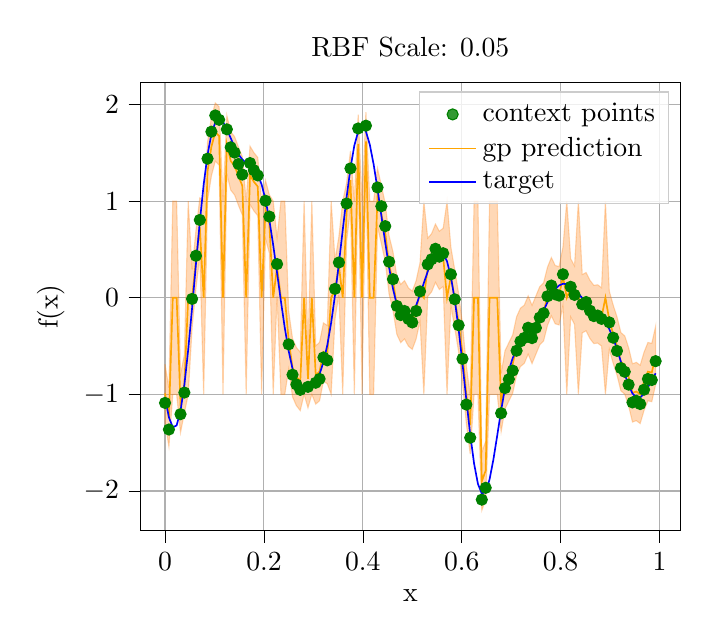
\begin{tikzpicture}

\definecolor{darkgray176}{RGB}{176,176,176}
\definecolor{darkorange25512714}{RGB}{255,127,14}
\definecolor{green}{RGB}{0,128,0}
\definecolor{lightgray204}{RGB}{204,204,204}
\definecolor{orange}{RGB}{255,165,0}

\begin{axis}[
legend cell align={left},
legend style={fill opacity=0.8, draw opacity=1, text opacity=1, draw=lightgray204},
tick align=outside,
tick pos=left,
title={RBF Scale: 0.05},
x grid style={darkgray176},
xlabel={x},
xmajorgrids,
xmin=-0.049609375, xmax=1.041796875,
xtick style={color=black},
y grid style={darkgray176},
ylabel={f(x)},
ymajorgrids,
ymin=-2.41224553995949, ymax=2.22731967114439,
ytick style={color=black}
]
\path [draw=darkorange25512714, fill=darkorange25512714, opacity=0.3]
(axis cs:0,-0.688383328985389)
--(axis cs:0,-1.29140601814092)
--(axis cs:0.0078125,-1.5413831705177)
--(axis cs:0.015625,-1)
--(axis cs:0.0234375,-1)
--(axis cs:0.03125,-1.39722157817871)
--(axis cs:0.0390625,-1.19397662668188)
--(axis cs:0.046875,-1)
--(axis cs:0.0546875,-0.312615969509551)
--(axis cs:0.0625,0.0932374694935545)
--(axis cs:0.0703125,0.430423814398134)
--(axis cs:0.078125,-1)
--(axis cs:0.0859375,1.00660140596913)
--(axis cs:0.09375,1.26045424831494)
--(axis cs:0.1015625,1.41340765421142)
--(axis cs:0.109375,1.37199936832405)
--(axis cs:0.1171875,-1)
--(axis cs:0.125,1.28255494331056)
--(axis cs:0.1328125,1.11365753849997)
--(axis cs:0.140625,1.06352678776651)
--(axis cs:0.1484375,0.956532171873315)
--(axis cs:0.15625,0.856964259341907)
--(axis cs:0.1640625,-1)
--(axis cs:0.171875,0.965423036921057)
--(axis cs:0.1796875,0.89815274910732)
--(axis cs:0.1875,0.8489957996014)
--(axis cs:0.1953125,-1)
--(axis cs:0.203125,0.610918073287938)
--(axis cs:0.2109375,0.461912394270764)
--(axis cs:0.21875,-1)
--(axis cs:0.2265625,0.0152650413264633)
--(axis cs:0.234375,-1)
--(axis cs:0.2421875,-1)
--(axis cs:0.25,-0.740297259312786)
--(axis cs:0.2578125,-1.02614532124722)
--(axis cs:0.265625,-1.11755500873782)
--(axis cs:0.2734375,-1.16809834347397)
--(axis cs:0.28125,-1)
--(axis cs:0.2890625,-1.13998389361326)
--(axis cs:0.296875,-1)
--(axis cs:0.3046875,-1.10139643136165)
--(axis cs:0.3125,-1.06571634374099)
--(axis cs:0.3203125,-0.863651326395437)
--(axis cs:0.328125,-0.890382622091687)
--(axis cs:0.3359375,-1)
--(axis cs:0.34375,-0.218288157083889)
--(axis cs:0.3515625,0.0299163128477336)
--(axis cs:0.359375,-1)
--(axis cs:0.3671875,0.584659180134388)
--(axis cs:0.375,0.915193592947601)
--(axis cs:0.3828125,-1)
--(axis cs:0.390625,1.290893798502)
--(axis cs:0.3984375,-1)
--(axis cs:0.40625,1.31714457989889)
--(axis cs:0.4140625,-1)
--(axis cs:0.421875,-1)
--(axis cs:0.4296875,0.735886932895363)
--(axis cs:0.4375,0.559125384839859)
--(axis cs:0.4453125,0.371735822723044)
--(axis cs:0.453125,0.0368862627547937)
--(axis cs:0.4609375,-0.127295112219921)
--(axis cs:0.46875,-0.378900165420577)
--(axis cs:0.4765625,-0.464845701930011)
--(axis cs:0.484375,-0.426493428332804)
--(axis cs:0.4921875,-0.50154131099667)
--(axis cs:0.5,-0.534409846037235)
--(axis cs:0.5078125,-0.426543569491712)
--(axis cs:0.515625,-0.241967819964512)
--(axis cs:0.5234375,-1)
--(axis cs:0.53125,0.0122248665430005)
--(axis cs:0.5390625,0.0602919132122145)
--(axis cs:0.546875,0.158896214718978)
--(axis cs:0.5546875,0.0846877741175106)
--(axis cs:0.5625,0.116868292496573)
--(axis cs:0.5703125,-1)
--(axis cs:0.578125,-0.0813338984325448)
--(axis cs:0.5859375,-0.316384265851202)
--(axis cs:0.59375,-0.560231258330496)
--(axis cs:0.6015625,-0.876462848827993)
--(axis cs:0.609375,-1.30663025659162)
--(axis cs:0.6171875,-1.61851670489081)
--(axis cs:0.625,-1)
--(axis cs:0.6328125,-1)
--(axis cs:0.640625,-2.20135621218204)
--(axis cs:0.6484375,-2.08992262848657)
--(axis cs:0.65625,-1)
--(axis cs:0.6640625,-1)
--(axis cs:0.671875,-1)
--(axis cs:0.6796875,-1.38823123426756)
--(axis cs:0.6875,-1.15162244906953)
--(axis cs:0.6953125,-1.06873940030507)
--(axis cs:0.703125,-0.987399313245003)
--(axis cs:0.7109375,-0.800413053019892)
--(axis cs:0.71875,-0.711758029811619)
--(axis cs:0.7265625,-0.679632507817893)
--(axis cs:0.734375,-0.583887351931207)
--(axis cs:0.7421875,-0.681631199463245)
--(axis cs:0.75,-0.584985494806654)
--(axis cs:0.7578125,-0.488159440646371)
--(axis cs:0.765625,-0.447267140033861)
--(axis cs:0.7734375,-0.287496374950949)
--(axis cs:0.78125,-0.186992655461015)
--(axis cs:0.7890625,-0.269502708169921)
--(axis cs:0.796875,-0.281603215293504)
--(axis cs:0.8046875,-0.0812010894034952)
--(axis cs:0.8125,-1)
--(axis cs:0.8203125,-0.198774182942497)
--(axis cs:0.828125,-0.275112009113055)
--(axis cs:0.8359375,-1)
--(axis cs:0.84375,-0.363647653058834)
--(axis cs:0.8515625,-0.34228646896296)
--(axis cs:0.859375,-0.423369229554881)
--(axis cs:0.8671875,-0.474572072217907)
--(axis cs:0.875,-0.469278532642914)
--(axis cs:0.8828125,-0.500621643663753)
--(axis cs:0.890625,-1)
--(axis cs:0.8984375,-0.53333254879791)
--(axis cs:0.90625,-0.677590134405544)
--(axis cs:0.9140625,-0.801608029662508)
--(axis cs:0.921875,-0.963462625849322)
--(axis cs:0.9296875,-0.998288812851843)
--(axis cs:0.9375,-1.1192513280054)
--(axis cs:0.9453125,-1.2865681735166)
--(axis cs:0.953125,-1.27205635452423)
--(axis cs:0.9609375,-1.3019123402926)
--(axis cs:0.96875,-1.16662625583365)
--(axis cs:0.9765625,-1.06622264929502)
--(axis cs:0.984375,-1.07593145893693)
--(axis cs:0.9921875,-0.898316631155426)
--(axis cs:0.9921875,-0.295293941999899)
--(axis cs:0.9921875,-0.295293941999899)
--(axis cs:0.984375,-0.472908769781403)
--(axis cs:0.9765625,-0.463199960139497)
--(axis cs:0.96875,-0.563603566678123)
--(axis cs:0.9609375,-0.698889651137071)
--(axis cs:0.953125,-0.669033665368699)
--(axis cs:0.9453125,-0.683545484361075)
--(axis cs:0.9375,-0.516228638849877)
--(axis cs:0.9296875,-0.395266123696316)
--(axis cs:0.921875,-0.360439936693794)
--(axis cs:0.9140625,-0.19858534050698)
--(axis cs:0.90625,-0.0745674452500167)
--(axis cs:0.8984375,0.0696901403576179)
--(axis cs:0.890625,1)
--(axis cs:0.8828125,0.102401045491775)
--(axis cs:0.875,0.133744156512613)
--(axis cs:0.8671875,0.12845061693762)
--(axis cs:0.859375,0.179653459600647)
--(axis cs:0.8515625,0.260736220192568)
--(axis cs:0.84375,0.239375036096694)
--(axis cs:0.8359375,1)
--(axis cs:0.828125,0.327910680042473)
--(axis cs:0.8203125,0.404248506213031)
--(axis cs:0.8125,1)
--(axis cs:0.8046875,0.521821599752032)
--(axis cs:0.796875,0.321419473862024)
--(axis cs:0.7890625,0.333519980985607)
--(axis cs:0.78125,0.416030033694513)
--(axis cs:0.7734375,0.315526314204578)
--(axis cs:0.765625,0.155755549121667)
--(axis cs:0.7578125,0.114863248509157)
--(axis cs:0.75,0.0180371943488732)
--(axis cs:0.7421875,-0.0786085103077172)
--(axis cs:0.734375,0.0191353372243203)
--(axis cs:0.7265625,-0.0766098186623656)
--(axis cs:0.71875,-0.108735340656092)
--(axis cs:0.7109375,-0.197390363864365)
--(axis cs:0.703125,-0.384376624089476)
--(axis cs:0.6953125,-0.465716711149538)
--(axis cs:0.6875,-0.548599759914007)
--(axis cs:0.6796875,-0.785208545112036)
--(axis cs:0.671875,1)
--(axis cs:0.6640625,1)
--(axis cs:0.65625,1)
--(axis cs:0.6484375,-1.48689993933105)
--(axis cs:0.640625,-1.59833352302651)
--(axis cs:0.6328125,1)
--(axis cs:0.625,1)
--(axis cs:0.6171875,-1.01549401573528)
--(axis cs:0.609375,-0.70360756743609)
--(axis cs:0.6015625,-0.273440159672465)
--(axis cs:0.59375,0.0427914308250313)
--(axis cs:0.5859375,0.286638423304326)
--(axis cs:0.578125,0.521688790722983)
--(axis cs:0.5703125,1)
--(axis cs:0.5625,0.719890981652101)
--(axis cs:0.5546875,0.687710463273038)
--(axis cs:0.546875,0.761918903874506)
--(axis cs:0.5390625,0.663314602367742)
--(axis cs:0.53125,0.615247555698528)
--(axis cs:0.5234375,1)
--(axis cs:0.515625,0.361054869191016)
--(axis cs:0.5078125,0.176479119663816)
--(axis cs:0.5,0.0686128431182931)
--(axis cs:0.4921875,0.101481378158857)
--(axis cs:0.484375,0.176529260822724)
--(axis cs:0.4765625,0.138176987225517)
--(axis cs:0.46875,0.224122523734951)
--(axis cs:0.4609375,0.475727576935606)
--(axis cs:0.453125,0.639908951910321)
--(axis cs:0.4453125,0.974758511878572)
--(axis cs:0.4375,1.16214807399539)
--(axis cs:0.4296875,1.33890962205089)
--(axis cs:0.421875,1)
--(axis cs:0.4140625,1)
--(axis cs:0.40625,1.92016726905442)
--(axis cs:0.3984375,1)
--(axis cs:0.390625,1.89391648765753)
--(axis cs:0.3828125,1)
--(axis cs:0.375,1.51821628210313)
--(axis cs:0.3671875,1.18768186928992)
--(axis cs:0.359375,1)
--(axis cs:0.3515625,0.632939002003261)
--(axis cs:0.34375,0.384734532071639)
--(axis cs:0.3359375,1)
--(axis cs:0.328125,-0.287359932936159)
--(axis cs:0.3203125,-0.260628637239909)
--(axis cs:0.3125,-0.462693654585458)
--(axis cs:0.3046875,-0.498373742206126)
--(axis cs:0.296875,1)
--(axis cs:0.2890625,-0.536961204457736)
--(axis cs:0.28125,1)
--(axis cs:0.2734375,-0.565075654318443)
--(axis cs:0.265625,-0.514532319582289)
--(axis cs:0.2578125,-0.423122632091688)
--(axis cs:0.25,-0.137274570157258)
--(axis cs:0.2421875,1)
--(axis cs:0.234375,1)
--(axis cs:0.2265625,0.618287730481991)
--(axis cs:0.21875,1)
--(axis cs:0.2109375,1.06493508342629)
--(axis cs:0.203125,1.21394076244347)
--(axis cs:0.1953125,1)
--(axis cs:0.1875,1.45201848875693)
--(axis cs:0.1796875,1.50117543826285)
--(axis cs:0.171875,1.56844572607658)
--(axis cs:0.1640625,1)
--(axis cs:0.15625,1.45998694849743)
--(axis cs:0.1484375,1.55955486102884)
--(axis cs:0.140625,1.66654947692204)
--(axis cs:0.1328125,1.7166802276555)
--(axis cs:0.125,1.88557763246609)
--(axis cs:0.1171875,1)
--(axis cs:0.109375,1.97502205747958)
--(axis cs:0.1015625,2.01643034336694)
--(axis cs:0.09375,1.86347693747047)
--(axis cs:0.0859375,1.60962409512466)
--(axis cs:0.078125,1)
--(axis cs:0.0703125,1.03344650355366)
--(axis cs:0.0625,0.696260158649082)
--(axis cs:0.0546875,0.290406719645977)
--(axis cs:0.046875,1)
--(axis cs:0.0390625,-0.590953937526351)
--(axis cs:0.03125,-0.794198889023184)
--(axis cs:0.0234375,1)
--(axis cs:0.015625,1)
--(axis cs:0.0078125,-0.938360481362176)
--(axis cs:0,-0.688383328985389)
--cycle;

\addplot [draw=green, fill=green, mark=*, only marks]
table{%
x  y
0 -1.08888411521912
0.0078125 -1.36385905742645
0.03125 -1.20528125762939
0.0390625 -0.981711804866791
0.0546875 -0.0122150871902704
0.0625 0.434223681688309
0.0703125 0.805128693580627
0.0859375 1.43892407417297
0.09375 1.71816217899323
0.1015625 1.88641095161438
0.109375 1.84086179733276
0.125 1.74247288703918
0.1328125 1.55668580532074
0.140625 1.50154197216034
0.1484375 1.38384783267975
0.15625 1.27432310581207
0.171875 1.39362776279449
0.1796875 1.31963050365448
0.1875 1.26555788516998
0.203125 1.0036723613739
0.2109375 0.839766085147858
0.2265625 0.348454028367996
0.25 -0.482664495706558
0.2578125 -0.797097384929657
0.265625 -0.89764803647995
0.2734375 -0.95324569940567
0.2890625 -0.922319829463959
0.3046875 -0.87987357378006
0.3125 -0.840625524520874
0.3203125 -0.618353962898254
0.328125 -0.647758424282074
0.34375 0.091545507311821
0.3515625 0.364570409059525
0.3671875 0.974787592887878
0.375 1.3383754491806
0.390625 1.75164568424225
0.40625 1.78052151203156
0.4296875 1.14113807678223
0.4375 0.946700394153595
0.4453125 0.740571856498718
0.453125 0.372237354516983
0.4609375 0.191637858748436
0.46875 -0.0851277038455009
0.4765625 -0.179667785763741
0.484375 -0.137480288743973
0.4921875 -0.220032960176468
0.5 -0.256188362836838
0.5078125 -0.137535452842712
0.515625 0.065497875213623
0.53125 0.345109820365906
0.5390625 0.397983580827713
0.546875 0.506448328495026
0.5546875 0.424819022417068
0.5625 0.460217595100403
0.578125 0.242195188999176
0.5859375 -0.0163602139800787
0.59375 -0.284591913223267
0.6015625 -0.632446646690369
0.609375 -1.1056307554245
0.6171875 -1.44870591163635
0.640625 -2.08982944488525
0.6484375 -1.96725237369537
0.6796875 -1.19539189338684
0.6875 -0.935122191905975
0.6953125 -0.843950867652893
0.703125 -0.75447678565979
0.7109375 -0.548791885375977
0.71875 -0.45127135515213
0.7265625 -0.415933281183243
0.734375 -0.310613602399826
0.7421875 -0.418131828308105
0.75 -0.311821579933167
0.7578125 -0.20531290769577
0.765625 -0.16033136844635
0.7734375 0.0154164666309953
0.78125 0.125970557332039
0.7890625 0.0352094992995262
0.796875 0.0218989420682192
0.8046875 0.242341279983521
0.8203125 0.113010875880718
0.828125 0.0290392693132162
0.84375 -0.0683499425649643
0.8515625 -0.0448526367545128
0.859375 -0.134043678641319
0.8671875 -0.190366804599762
0.875 -0.184543907642365
0.8828125 -0.219021335244179
0.8984375 -0.255003333091736
0.90625 -0.413686662912369
0.9140625 -0.550106346607208
0.921875 -0.728146433830261
0.9296875 -0.766455233097076
0.9375 -0.899513959884644
0.9453125 -1.08356249332428
0.953125 -1.0675995349884
0.9609375 -1.1004410982132
0.96875 -0.951626420021057
0.9765625 -0.84118241071701
0.984375 -0.851862132549286
0.9921875 -0.656485795974731
};
\addlegendentry{context points}
\addplot [semithick, orange]
table {%
0 -0.989894673563153
0.0078125 -1.23987182593994
0.015625 -8.63182962435564e-81
0.0234375 -7.62819499260482e-81
0.03125 -1.09571023360095
0.0390625 -0.892465282104115
0.046875 -6.29053852829941e-81
0.0546875 -0.0111046249317873
0.0625 0.394748814071318
0.0703125 0.731935158975898
0.078125 1.42025535318319e-80
0.0859375 1.30811275054689
0.09375 1.56196559289271
0.1015625 1.71491899878918
0.109375 1.67351071290182
0.1171875 2.26788358850887e-80
0.125 1.58406628788832
0.1328125 1.41516888307773
0.140625 1.36503813234428
0.1484375 1.25804351645108
0.15625 1.15847560391967
0.1640625 1.68853951879024e-80
0.171875 1.26693438149882
0.1796875 1.19966409368508
0.1875 1.15050714417916
0.1953125 1.43619014134169e-80
0.203125 0.912429417865702
0.2109375 0.763423738848528
0.21875 7.5202155916508e-81
0.2265625 0.316776385904227
0.234375 2.20535682393606e-81
0.2421875 -3.05477161294021e-81
0.25 -0.438785914735022
0.2578125 -0.724633976669452
0.265625 -0.816043664160053
0.2734375 -0.866586998896207
0.28125 -1.18704072543765e-80
0.2890625 -0.8384725490355
0.296875 -1.14060370437407e-80
0.3046875 -0.79988508678389
0.3125 -0.764204999163222
0.3203125 -0.562139981817673
0.328125 -0.588871277513923
0.3359375 -3.52025755535937e-81
0.34375 0.0832231874938751
0.3515625 0.331427657425497
0.359375 8.47676335509911e-81
0.3671875 0.886170524712152
0.375 1.21670493752536
0.3828125 1.95566663460928e-80
0.390625 1.59240514307976
0.3984375 2.23549978866154e-80
0.40625 1.61865592447665
0.4140625 1.12688762404417e-80
0.421875 7.22223458620296e-81
0.4296875 1.03739827747313
0.4375 0.860636729417622
0.4453125 0.673247167300808
0.453125 0.338397607332558
0.4609375 0.174216232357843
0.46875 -0.0773888208428133
0.4765625 -0.163334357352247
0.484375 -0.12498208375504
0.4921875 -0.200029966418907
0.5 -0.232898501459471
0.5078125 -0.125032224913948
0.515625 0.0595435246132523
0.5234375 2.59872594381364e-81
0.53125 0.313736211120764
0.5390625 0.361803257789978
0.546875 0.460407559296742
0.5546875 0.386199118695274
0.5625 0.418379637074337
0.5703125 4.44555302608877e-81
0.578125 0.220177446145219
0.5859375 -0.0148729212734377
0.59375 -0.258719913752733
0.6015625 -0.574951504250229
0.609375 -1.00511891201385
0.6171875 -1.31700536031305
0.625 -9.1688234596225e-81
0.6328125 -1.32264778235929e-80
0.640625 -1.89984486760428
0.6484375 -1.78841128390881
0.65625 -1.24506914166145e-80
0.6640625 -6.74399606573302e-321
0.671875 -7.56560536413778e-81
0.6796875 -1.0867198896898
0.6875 -0.850111104491771
0.6953125 -0.767228055727302
0.703125 -0.68588796866724
0.7109375 -0.498901708442128
0.71875 -0.410246685233856
0.7265625 -0.378121163240129
0.734375 -0.282376007353444
0.7421875 -0.380119854885481
0.75 -0.283474150228891
0.7578125 -0.186648096068607
0.765625 -0.145755795456097
0.7734375 0.0140149696268144
0.78125 0.114518689116749
0.7890625 0.0320086364078432
0.796875 0.0199081292842603
0.8046875 0.220310255174269
0.8125 2.2490149418296e-81
0.8203125 0.102737161635267
0.828125 0.0263993354647092
0.8359375 -2.48796251285932e-82
0.84375 -0.0621363084810699
0.8515625 -0.0407751243851963
0.859375 -0.121857884977117
0.8671875 -0.173060727640144
0.875 -0.16776718806515
0.8828125 -0.199110299085989
0.890625 -3.00009020165606e-81
0.8984375 -0.231821204220146
0.90625 -0.376078789827781
0.9140625 -0.500096685084744
0.921875 -0.661951281271558
0.9296875 -0.69677746827408
0.9375 -0.817739983427641
0.9453125 -0.985056828938838
0.953125 -0.970545009946463
0.9609375 -1.00040099571483
0.96875 -0.865114911255886
0.9765625 -0.764711304717261
0.984375 -0.774420114359166
0.9921875 -0.596805286577663
};
\addlegendentry{gp prediction}
\addplot [semithick, blue]
table {%
0 -1.03190088272095
0.0078125 -1.23832082748413
0.015625 -1.34114527702332
0.0234375 -1.32112503051758
0.03125 -1.17219460010529
0.0390625 -0.903067886829376
0.046875 -0.536460399627686
0.0546875 -0.106029771268368
0.0625 0.348389685153961
0.0703125 0.786377489566803
0.078125 1.17235600948334
0.0859375 1.47996890544891
0.09375 1.69477891921997
0.1015625 1.81499648094177
0.109375 1.85029745101929
0.1171875 1.81907176971436
0.125 1.74464392662048
0.1328125 1.65108573436737
0.140625 1.5592485666275
0.1484375 1.48356473445892
0.15625 1.43004608154297
0.1640625 1.39574778079987
0.171875 1.36977696418762
0.1796875 1.33572459220886
0.1875 1.27517974376678
0.1953125 1.17177939414978
0.203125 1.01506853103638
0.2109375 0.803369522094727
0.21875 0.544939458370209
0.2265625 0.256988525390625
0.234375 -0.0373827256262302
0.2421875 -0.31369349360466
0.25 -0.550928950309753
0.2578125 -0.735419094562531
0.265625 -0.862659752368927
0.2734375 -0.936571002006531
0.28125 -0.966469764709473
0.2890625 -0.962743639945984
0.296875 -0.932617247104645
0.3046875 -0.877354919910431
0.3125 -0.79178786277771
0.3203125 -0.666325271129608
0.328125 -0.490849494934082
0.3359375 -0.259326338768005
0.34375 0.0262537952512503
0.3515625 0.353797823190689
0.359375 0.701548218727112
0.3671875 1.04097235202789
0.375 1.34135222434998
0.3828125 1.57489681243896
0.390625 1.72113740444183
0.3984375 1.76968026161194
0.40625 1.72093117237091
0.4140625 1.5849871635437
0.421875 1.37929701805115
0.4296875 1.12583386898041
0.4375 0.848393142223358
0.4453125 0.570347785949707
0.453125 0.312901496887207
0.4609375 0.0937184765934944
0.46875 -0.0741947144269943
0.4765625 -0.183340907096863
0.484375 -0.232152581214905
0.4921875 -0.224762991070747
0.5 -0.170023009181023
0.5078125 -0.0799106359481812
0.515625 0.0322536490857601
0.5234375 0.153246462345123
0.53125 0.270607441663742
0.5390625 0.372446179389954
0.546875 0.446724712848663
0.5546875 0.480664193630219
0.5625 0.460967868566513
0.5703125 0.375286787748337
0.578125 0.214874431490898
0.5859375 -0.0221472587436438
0.59375 -0.327864438295364
0.6015625 -0.683051466941833
0.609375 -1.057896733284
0.6171875 -1.41531252861023
0.625 -1.71648979187012
0.6328125 -1.92767524719238
0.640625 -2.0266592502594
0.6484375 -2.00734686851501
0.65625 -1.88113224506378
0.6640625 -1.67455267906189
0.671875 -1.42367446422577
0.6796875 -1.16656041145325
0.6875 -0.935693144798279
0.6953125 -0.752215683460236
0.703125 -0.623294651508331
0.7109375 -0.542998433113098
0.71875 -0.496118426322937
0.7265625 -0.463622778654099
0.734375 -0.428145885467529
0.7421875 -0.378092586994171
0.75 -0.309508740901947
0.7578125 -0.22560116648674
0.765625 -0.13447293639183
0.7734375 -0.0460650362074375
0.78125 0.0306433904916048
0.7890625 0.089411273598671
0.796875 0.127238944172859
0.8046875 0.143865555524826
0.8125 0.140849381685257
0.8203125 0.120811343193054
0.828125 0.0871279388666153
0.8359375 0.0439450740814209
0.84375 -0.0039005228318274
0.8515625 -0.0514686331152916
0.859375 -0.0949170738458633
0.8671875 -0.132983282208443
0.875 -0.168070718646049
0.8828125 -0.206248894333839
0.890625 -0.255822032690048
0.8984375 -0.324701368808746
0.90625 -0.417362183332443
0.9140625 -0.532440483570099
0.921875 -0.661884367465973
0.9296875 -0.792080819606781
0.9375 -0.906728088855743
0.9453125 -0.99066162109375
0.953125 -1.03355658054352
0.9609375 -1.03250002861023
0.96875 -0.992771685123444
0.9765625 -0.926686108112335
0.984375 -0.850848078727722
0.9921875 -0.782549917697906
};
\addlegendentry{target}
\end{axis}

\end{tikzpicture}

	}
\end{figure}

	\begin{figure}
	\centering
	\resizebox{0.95\textwidth}{!}{
		% This file was created with matplot2tikz v0.4.0.
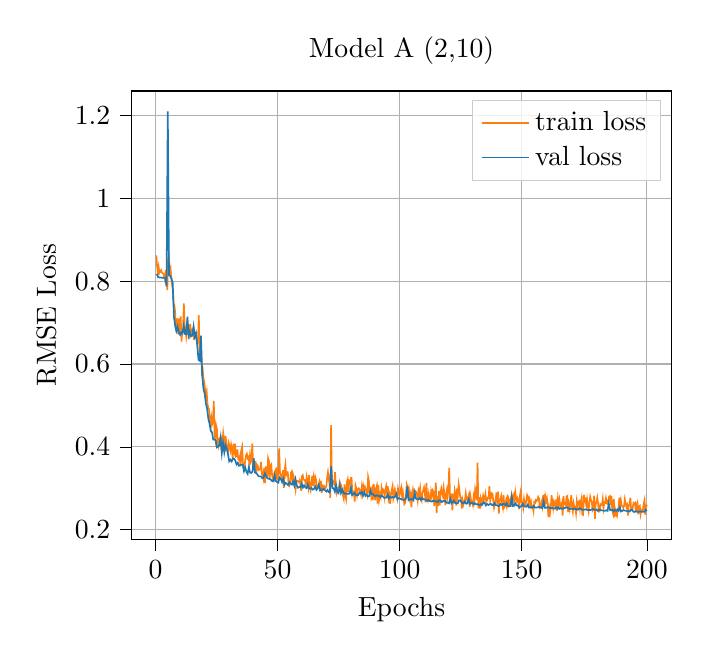
\begin{tikzpicture}

\definecolor{darkgray176}{RGB}{176,176,176}
\definecolor{darkorange25512714}{RGB}{255,127,14}
\definecolor{lightgray204}{RGB}{204,204,204}
\definecolor{steelblue31119180}{RGB}{31,119,180}


\begin{axis}[
scaled ticks=false,
legend cell align={left},
legend style={fill opacity=0.8, draw opacity=1, text opacity=1, draw=lightgray204},
tick align=outside,
tick pos=left,
title={Model A (2,10)},
x grid style={darkgray176},
xlabel={Epochs},
xmajorgrids,
xmin=-1508.5, xmax=32756.5,
xtick style={color=black},
xtick={0,7750,15500,23250,31200},
xticklabels={0,50,100,150,200},
y grid style={darkgray176},
ylabel={RMSE Loss},
ymajorgrids,
ymin=0.176929806172848, ymax=1.25942015200853,
ytick style={color=black}
]
\addplot [semithick, darkorange25512714]
table {%
49 0.862413883209229
99 0.836784839630127
149 0.820097684860229
199 0.834237694740295
249 0.820140719413757
299 0.823864698410034
349 0.826734304428101
399 0.821079254150391
449 0.819839477539062
499 0.817773461341858
549 0.812215328216553
599 0.803227186203003
649 0.827330112457275
699 0.804917097091675
749 0.778725385665894
799 0.852275013923645
849 0.859122037887573
899 0.827279567718506
949 0.831976175308228
1049 0.792464852333069
1099 0.778606057167053
1149 0.744878530502319
1199 0.742368936538696
1249 0.72347617149353
1299 0.679774403572083
1399 0.710126399993896
1449 0.671633243560791
1499 0.710426568984985
1549 0.671138525009155
1599 0.714828968048096
1649 0.654139995574951
1699 0.678018808364868
1749 0.685258269309998
1799 0.74622118473053
1849 0.694862723350525
1899 0.683924436569214
1949 0.667033314704895
1999 0.686914443969727
2049 0.670249462127686
2099 0.694721937179565
2149 0.660601615905762
2199 0.697094440460205
2249 0.676736354827881
2299 0.683452129364014
2349 0.684104561805725
2399 0.686967730522156
2449 0.658705234527588
2499 0.6739342212677
2549 0.669074177742004
2599 0.661392092704773
2649 0.649881482124329
2699 0.653015851974487
2749 0.717896223068237
2799 0.622180938720703
2849 0.619962215423584
2899 0.630519390106201
2949 0.580384492874146
2999 0.585428714752197
3049 0.562883257865906
3099 0.556499719619751
3149 0.536479949951172
3199 0.521177291870117
3249 0.532508611679077
3299 0.504068374633789
3349 0.493211388587952
3399 0.491312265396118
3449 0.466556549072266
3499 0.45128059387207
3549 0.470323443412781
3599 0.456472635269165
3649 0.464459180831909
3699 0.511225581169128
3749 0.429898619651794
3799 0.418075799942017
3849 0.451286673545837
3899 0.442596912384033
3949 0.409034371376038
3999 0.40170693397522
4049 0.419798493385315
4099 0.421337246894836
4149 0.405456185340881
4199 0.417596101760864
4249 0.409929871559143
4299 0.432628750801086
4349 0.416831612586975
4399 0.387445688247681
4449 0.426348447799683
4499 0.408865571022034
4549 0.396186470985413
4599 0.388407230377197
4649 0.408631801605225
4699 0.400671601295471
4749 0.39088249206543
4799 0.404917240142822
4849 0.393564939498901
4899 0.372330784797668
4949 0.407837867736816
4999 0.392922878265381
5049 0.407784819602966
5099 0.376586198806763
5149 0.377859950065613
5199 0.394073843955994
5249 0.370936751365662
5299 0.36875057220459
5349 0.376378536224365
5399 0.353736519813538
5449 0.392664432525635
5499 0.400428056716919
5549 0.361891865730286
5599 0.353745222091675
5649 0.351234555244446
5699 0.367599248886108
5749 0.379606366157532
5799 0.383235573768616
5849 0.372769117355347
5899 0.375554800033569
5949 0.363500118255615
5999 0.380848169326782
6049 0.363919973373413
6099 0.369454503059387
6149 0.408167362213135
6199 0.345090389251709
6249 0.35671603679657
6299 0.349497318267822
6349 0.365665674209595
6399 0.336077570915222
6449 0.356389999389648
6499 0.353447914123535
6549 0.344269871711731
6599 0.345422267913818
6649 0.345526218414307
6699 0.363441705703735
6749 0.335713505744934
6799 0.337982892990112
6849 0.326171159744263
6899 0.348966360092163
6949 0.312571406364441
6999 0.350863456726074
7049 0.351192951202393
7099 0.327701330184937
7149 0.372661828994751
7199 0.366609573364258
7249 0.322076916694641
7299 0.355439901351929
7349 0.357875943183899
7399 0.332801818847656
7449 0.321600317955017
7499 0.318665504455566
7549 0.33849835395813
7599 0.342206239700317
7649 0.321833252906799
7699 0.350178241729736
7749 0.335832834243774
7799 0.320318937301636
7849 0.396325349807739
7899 0.342136144638062
7949 0.334157109260559
7999 0.324594736099243
8049 0.318691372871399
8099 0.343600630760193
8149 0.301064968109131
8199 0.342776417732239
8249 0.356741905212402
8299 0.333385467529297
8349 0.339282274246216
8399 0.338810086250305
8449 0.309496760368347
8499 0.306409120559692
8549 0.313758134841919
8599 0.337136149406433
8649 0.340588688850403
8699 0.314509391784668
8749 0.330944895744324
8799 0.323974609375
8849 0.31769323348999
8899 0.299188852310181
8949 0.317760705947876
8999 0.317934274673462
9049 0.316534280776978
9099 0.31525731086731
9149 0.319430112838745
9199 0.309981346130371
9249 0.293971180915833
9299 0.329241394996643
9349 0.33156406879425
9399 0.321075439453125
9449 0.320910453796387
9499 0.317725777626038
9549 0.309439539909363
9599 0.327704548835754
9649 0.316954970359802
9699 0.303776144981384
9749 0.331490278244019
9799 0.30102801322937
9849 0.294941067695618
9899 0.311160922050476
9949 0.330424189567566
9999 0.3054119348526
10049 0.327438116073608
10099 0.316349864006042
10149 0.32678484916687
10199 0.319643020629883
10249 0.300944089889526
10299 0.301677703857422
10349 0.307106494903564
10399 0.314298748970032
10449 0.29265820980072
10499 0.318429350852966
10549 0.289097547531128
10599 0.306135654449463
10649 0.303159594535828
10699 0.305373668670654
10749 0.299092888832092
10799 0.300715804100037
10849 0.304946184158325
10899 0.326815843582153
10949 0.339032053947449
10999 0.323649525642395
11049 0.308890342712402
11099 0.276707410812378
11149 0.452712297439575
11199 0.303796410560608
11249 0.314051508903503
11299 0.316434144973755
11349 0.311334133148193
11399 0.338758826255798
11449 0.300090432167053
11499 0.289675712585449
11549 0.301256418228149
11599 0.301756620407104
11649 0.301620841026306
11699 0.315196871757507
11749 0.309532284736633
11799 0.306942582130432
11849 0.29587185382843
11899 0.28313672542572
11949 0.275025963783264
11999 0.309078693389893
12049 0.284453868865967
12099 0.274876356124878
12149 0.314593434333801
12199 0.321276903152466
12249 0.290569067001343
12299 0.316218376159668
12349 0.313213706016541
12399 0.324894070625305
12449 0.325338125228882
12499 0.286268591880798
12549 0.292208313941956
12599 0.290031909942627
12649 0.26790463924408
12699 0.306963205337524
12749 0.300013542175293
12799 0.284244179725647
12849 0.298034906387329
12899 0.299904584884644
12949 0.297329068183899
12999 0.29280161857605
13049 0.284981608390808
13099 0.303407192230225
13149 0.28845226764679
13199 0.305415034294128
13249 0.296996116638184
13299 0.303386688232422
13349 0.298430442810059
13399 0.29060971736908
13449 0.283275365829468
13499 0.326751470565796
13549 0.316812515258789
13599 0.285865783691406
13649 0.303849577903748
13699 0.281580686569214
13749 0.292229056358337
13799 0.270811200141907
13849 0.310732364654541
13899 0.290295600891113
13949 0.271133661270142
13999 0.299466371536255
14049 0.306306958198547
14099 0.263170480728149
14149 0.307638049125671
14199 0.273392200469971
14249 0.285097599029541
14299 0.278789043426514
14349 0.300557613372803
14399 0.289375424385071
14449 0.297252058982849
14499 0.294884920120239
14549 0.279208183288574
14599 0.298005819320679
14649 0.305830836296082
14699 0.29063606262207
14749 0.305254459381104
14799 0.275246143341064
14849 0.283949494361877
14899 0.262596368789673
14949 0.284632444381714
14999 0.29582405090332
15049 0.304943323135376
15099 0.276071071624756
15149 0.285475015640259
15199 0.296772956848145
15249 0.287038922309875
15299 0.284144997596741
15349 0.275277614593506
15399 0.299320220947266
15449 0.290938854217529
15499 0.283428430557251
15549 0.2930908203125
15599 0.301813006401062
15649 0.282862663269043
15699 0.291936993598938
15749 0.27539587020874
15799 0.261659383773804
15849 0.264327883720398
15899 0.281185626983643
15949 0.309489369392395
15999 0.303490877151489
16049 0.275934815406799
16099 0.293727159500122
16149 0.27575945854187
16199 0.285559296607971
16249 0.254119515419006
16299 0.28408145904541
16349 0.297262907028198
16399 0.287301301956177
16449 0.293452024459839
16499 0.293448209762573
16549 0.291307926177979
16599 0.286740303039551
16649 0.271992683410645
16699 0.294326066970825
16749 0.286872029304504
16799 0.299620389938354
16849 0.274327158927917
16899 0.269679069519043
16949 0.289080262184143
16999 0.29509699344635
17049 0.301992893218994
17099 0.289722323417664
17149 0.265834808349609
17199 0.313076853752136
17249 0.279711008071899
17299 0.272167563438416
17349 0.285445094108582
17399 0.27077841758728
17449 0.269371509552002
17499 0.291646122932434
17549 0.282899856567383
17599 0.295307636260986
17649 0.292267799377441
17699 0.257309794425964
17749 0.27709698677063
17799 0.313453674316406
17849 0.240280866622925
17899 0.281322956085205
17949 0.257058382034302
17999 0.293950438499451
18049 0.259070515632629
18099 0.290685892105103
18149 0.299850463867188
18199 0.288699746131897
18249 0.280828237533569
18299 0.300952434539795
18349 0.286361455917358
18399 0.25973904132843
18449 0.283588528633118
18499 0.295714497566223
18549 0.279741048812866
18599 0.299014806747437
18649 0.34925651550293
18699 0.279833078384399
18749 0.283280611038208
18799 0.28478741645813
18849 0.246931076049805
18899 0.286177396774292
18949 0.264474511146545
18999 0.294249296188354
19049 0.284403562545776
19099 0.258190035820007
19149 0.299426078796387
19199 0.284655213356018
19249 0.308587789535522
19299 0.294289588928223
19349 0.278008937835693
19399 0.277700543403625
19449 0.251278877258301
19499 0.270854592323303
19549 0.261157631874084
19599 0.268452882766724
19649 0.272309064865112
19699 0.287688374519348
19749 0.273220539093018
19799 0.271107792854309
19849 0.277843952178955
19899 0.284416675567627
19949 0.255105018615723
19999 0.279952883720398
20049 0.268282055854797
20099 0.266216993331909
20149 0.259380102157593
20199 0.279698967933655
20249 0.269780397415161
20299 0.298248887062073
20349 0.289122462272644
20399 0.27161693572998
20449 0.361763119697571
20499 0.251341104507446
20549 0.278523325920105
20599 0.250897169113159
20649 0.273790717124939
20699 0.263675570487976
20749 0.27245557308197
20799 0.281762599945068
20849 0.270842790603638
20899 0.277294635772705
20949 0.286748886108398
20999 0.267761945724487
21049 0.270815372467041
21099 0.276916742324829
21149 0.276427268981934
21199 0.304862022399902
21249 0.270267009735107
21299 0.277698636054993
21349 0.28804075717926
21399 0.286165237426758
21449 0.268922209739685
21499 0.253375768661499
21549 0.26274585723877
21599 0.273878574371338
21649 0.289990901947021
21699 0.262274503707886
21749 0.292029500007629
21799 0.239112615585327
21849 0.269742846488953
21899 0.274371862411499
21949 0.281761646270752
21999 0.265287756919861
22049 0.254708528518677
22099 0.284090995788574
22149 0.254441976547241
22199 0.257907509803772
22249 0.268370866775513
22299 0.257923603057861
22349 0.284487724304199
22399 0.254156231880188
22449 0.27063000202179
22499 0.263018608093262
22549 0.272271513938904
22599 0.281397461891174
22649 0.254973530769348
22699 0.280713081359863
22749 0.285328269004822
22799 0.270806908607483
22849 0.289667129516602
22899 0.275566458702087
22949 0.26899790763855
22999 0.276117920875549
23049 0.270693778991699
23099 0.248999357223511
23149 0.284989595413208
23199 0.29479193687439
23249 0.266525030136108
23299 0.265896320343018
23349 0.253974437713623
23399 0.273823618888855
23449 0.262897253036499
23499 0.260626792907715
23549 0.271186113357544
23599 0.283634543418884
23649 0.279525756835938
23699 0.264202117919922
23749 0.272592067718506
23799 0.258236408233643
23849 0.266207337379456
23899 0.253995418548584
23949 0.255951046943665
23999 0.245450973510742
24049 0.266610145568848
24099 0.264748454093933
24149 0.271581649780273
24199 0.269286274909973
24249 0.271798729896545
24299 0.279275417327881
24349 0.275332689285278
24399 0.253250122070312
24449 0.254563808441162
24499 0.264630198478699
24549 0.255519509315491
24599 0.281217932701111
24649 0.282375812530518
24699 0.258708477020264
24749 0.28032660484314
24799 0.269406318664551
24849 0.276383519172668
24899 0.260939002037048
24949 0.230556130409241
24999 0.251450777053833
25049 0.239818811416626
25099 0.254084229469299
25149 0.283605813980103
25199 0.263538599014282
25249 0.251838445663452
25299 0.26848566532135
25349 0.263192772865295
25399 0.256482720375061
25449 0.273657321929932
25499 0.245606064796448
25549 0.274600744247437
25599 0.260852813720703
25649 0.272472143173218
25699 0.257571578025818
25749 0.25470495223999
25799 0.26277756690979
25849 0.234274506568909
25899 0.281277418136597
25949 0.262167811393738
25999 0.263323783874512
26049 0.259234309196472
26099 0.28016984462738
26149 0.281479835510254
26199 0.242525815963745
26249 0.260502576828003
26299 0.249786019325256
26349 0.267346858978271
26399 0.283116102218628
26449 0.255717515945435
26499 0.243843793869019
26549 0.263163328170776
26599 0.253117680549622
26649 0.25438117980957
26699 0.240290403366089
26749 0.268191337585449
26799 0.256289958953857
26849 0.266801595687866
26899 0.268778562545776
26949 0.251124739646912
26999 0.266262054443359
27049 0.275528192520142
27099 0.237073540687561
27149 0.235829830169678
27199 0.284324526786804
27249 0.268991351127625
27299 0.272384166717529
27349 0.259145736694336
27399 0.272992014884949
27449 0.256349325180054
27499 0.245213031768799
27549 0.266211271286011
27599 0.279416561126709
27649 0.271238684654236
27699 0.26775336265564
27749 0.247034192085266
27799 0.250554800033569
27849 0.281991839408875
27899 0.226133942604065
27949 0.26195764541626
27999 0.267517685890198
28049 0.277435779571533
28099 0.263699412345886
28149 0.243626713752747
28199 0.24379301071167
28249 0.261795282363892
28299 0.260099172592163
28349 0.259344339370728
28399 0.274008989334106
28449 0.252649068832397
28499 0.265744686126709
28549 0.264849185943604
28599 0.275921940803528
28649 0.26403546333313
28699 0.262134671211243
28749 0.270555019378662
28799 0.279731273651123
28849 0.281272649765015
28899 0.259418845176697
28949 0.2816162109375
28999 0.24738073348999
29049 0.239478588104248
29099 0.274532437324524
29149 0.230533480644226
29199 0.24583375453949
29249 0.236605763435364
29299 0.232761383056641
29349 0.24980640411377
29399 0.25245726108551
29449 0.277435779571533
29499 0.256390333175659
29549 0.270865917205811
29599 0.25847852230072
29649 0.256513833999634
29699 0.252711772918701
29749 0.256601452827454
29799 0.273590087890625
29849 0.264134764671326
29899 0.255703330039978
29949 0.25989556312561
29999 0.234219312667847
30049 0.259397029876709
30099 0.259180545806885
30149 0.277147889137268
30199 0.250317096710205
30249 0.247665524482727
30299 0.25239634513855
30349 0.264201283454895
30399 0.261746406555176
30449 0.264408826828003
30499 0.2420574426651
30549 0.260393142700195
30599 0.265455007553101
30649 0.237151384353638
30699 0.255824565887451
30749 0.257764339447021
30799 0.237851858139038
30849 0.248220562934875
30899 0.247461915016174
30949 0.24727737903595
30999 0.26340115070343
31049 0.271576166152954
31099 0.236292123794556
31149 0.254941582679749
31199 0.260451316833496
};
\addlegendentry{train loss}
\addplot [semithick, steelblue31119180]
table {%
77 0.817664861679077
155 0.810476779937744
233 0.808972477912903
311 0.809321403503418
389 0.808443069458008
467 0.807960987091064
545 0.808243989944458
623 0.808139562606812
701 0.787868022918701
779 1.21021604537964
857 0.814702272415161
935 0.812561750411987
1013 0.805981516838074
1091 0.796039581298828
1169 0.71419095993042
1247 0.692407846450806
1325 0.679630041122437
1403 0.690068960189819
1481 0.675244569778442
1559 0.670684814453125
1637 0.676871418952942
1715 0.67397141456604
1793 0.692445755004883
1871 0.672709941864014
1949 0.671869039535522
2027 0.714231371879578
2105 0.668651342391968
2183 0.678156852722168
2261 0.666807174682617
2339 0.668517351150513
2417 0.690611362457275
2495 0.666260480880737
2573 0.674643993377686
2651 0.644995450973511
2729 0.610462188720703
2807 0.608117341995239
2885 0.668771982192993
2963 0.574352979660034
3041 0.540813446044922
3119 0.529028654098511
3197 0.505244970321655
3275 0.492183208465576
3353 0.468250155448914
3431 0.455799579620361
3509 0.438636898994446
3587 0.435343146324158
3665 0.417929887771606
3743 0.417998075485229
3821 0.41644012928009
3899 0.398920059204102
3977 0.401051998138428
4055 0.403836607933044
4133 0.422684073448181
4211 0.385217308998108
4289 0.409080505371094
4367 0.386908411979675
4445 0.403984308242798
4523 0.395946979522705
4601 0.382471680641174
4679 0.365227580070496
4757 0.369128465652466
4835 0.364861726760864
4913 0.371886730194092
4991 0.371472120285034
5069 0.366852164268494
5147 0.357492208480835
5225 0.361699104309082
5303 0.354348182678223
5381 0.355725169181824
5459 0.357224464416504
5537 0.357190608978271
5615 0.341452717781067
5693 0.350429058074951
5771 0.34000289440155
5849 0.334920763969421
5927 0.351287961006165
6005 0.33779764175415
6083 0.337132215499878
6161 0.340792059898376
6239 0.372683763504028
6317 0.337894439697266
6395 0.336796760559082
6473 0.333069562911987
6551 0.328731298446655
6629 0.328808069229126
6707 0.328718781471252
6785 0.324338793754578
6863 0.326165318489075
6941 0.336180210113525
7019 0.330429434776306
7097 0.324375987052917
7175 0.322977542877197
7253 0.322561144828796
7331 0.32046914100647
7409 0.317299365997314
7487 0.316826105117798
7565 0.330967307090759
7643 0.317682981491089
7721 0.314884424209595
7799 0.313461661338806
7877 0.325826168060303
7955 0.322529911994934
8033 0.315348625183105
8111 0.322973132133484
8189 0.308667302131653
8267 0.312951803207397
8345 0.310508489608765
8423 0.307454109191895
8501 0.31438422203064
8579 0.311030626296997
8657 0.309033632278442
8735 0.31635844707489
8813 0.306121587753296
8891 0.321569085121155
8969 0.306983351707458
9047 0.301435589790344
9125 0.303032159805298
9203 0.302685856819153
9281 0.311602115631104
9359 0.302019357681274
9437 0.306963324546814
9515 0.302188515663147
9593 0.300373554229736
9671 0.309417724609375
9749 0.299891710281372
9827 0.299054503440857
9905 0.300502777099609
9983 0.296937227249146
10061 0.298284769058228
10139 0.304667592048645
10217 0.296235203742981
10295 0.299856185913086
10373 0.308019876480103
10451 0.295146942138672
10529 0.29731011390686
10607 0.295497417449951
10685 0.298752546310425
10763 0.295133829116821
10841 0.292124032974243
10919 0.295958280563354
10997 0.290807604789734
11075 0.291584014892578
11153 0.353235602378845
11231 0.300697326660156
11309 0.300139784812927
11387 0.291935682296753
11465 0.307579159736633
11543 0.290753960609436
11621 0.288146734237671
11699 0.306883573532104
11777 0.288962960243225
11855 0.296632170677185
11933 0.289595127105713
12011 0.286815524101257
12089 0.28744900226593
12167 0.286450266838074
12245 0.286435127258301
12323 0.287057757377625
12401 0.301676034927368
12479 0.284043908119202
12557 0.285333275794983
12635 0.289117693901062
12713 0.283149480819702
12791 0.28326427936554
12869 0.283786296844482
12947 0.289608597755432
13025 0.287389039993286
13103 0.291091442108154
13181 0.28259539604187
13259 0.29084575176239
13337 0.28171181678772
13415 0.28371000289917
13493 0.280213952064514
13571 0.281321287155151
13649 0.294035196304321
13727 0.285523056983948
13805 0.285978078842163
13883 0.282775163650513
13961 0.281063199043274
14039 0.283217310905457
14117 0.281729102134705
14195 0.28192663192749
14273 0.278913021087646
14351 0.282656073570251
14429 0.280107259750366
14507 0.277080535888672
14585 0.277333498001099
14663 0.277456283569336
14741 0.285247325897217
14819 0.275621652603149
14897 0.2793790102005
14975 0.277329206466675
15053 0.278894901275635
15131 0.277351498603821
15209 0.279870748519897
15287 0.286622285842896
15365 0.273694634437561
15443 0.276440620422363
15521 0.274755001068115
15599 0.274191498756409
15677 0.272441029548645
15755 0.272176742553711
15833 0.272202610969543
15911 0.276858329772949
15989 0.304653882980347
16067 0.271635293960571
16145 0.274387359619141
16223 0.272396564483643
16301 0.274676203727722
16379 0.271180629730225
16457 0.289785861968994
16535 0.27541971206665
16613 0.273374080657959
16691 0.273280143737793
16769 0.276687383651733
16847 0.271892547607422
16925 0.276639223098755
17003 0.273638367652893
17081 0.273130655288696
17159 0.272330403327942
17237 0.269223213195801
17315 0.27192211151123
17393 0.269215106964111
17471 0.269020795822144
17549 0.267986536026001
17627 0.270293593406677
17705 0.269922971725464
17783 0.267749786376953
17861 0.269218444824219
17939 0.266875505447388
18017 0.271280288696289
18095 0.270978450775146
18173 0.266765356063843
18251 0.269158601760864
18329 0.269342064857483
18407 0.269200801849365
18485 0.265044569969177
18563 0.265523791313171
18641 0.263875722885132
18719 0.27432918548584
18797 0.263653755187988
18875 0.26632285118103
18953 0.269991874694824
19031 0.26442277431488
19109 0.26380443572998
19187 0.263558626174927
19265 0.2703697681427
19343 0.271199703216553
19421 0.266963601112366
19499 0.263847231864929
19577 0.263956189155579
19655 0.268267035484314
19733 0.262802958488464
19811 0.263822674751282
19889 0.273395657539368
19967 0.262372851371765
20045 0.264018058776855
20123 0.265174746513367
20201 0.261213660240173
20279 0.264276146888733
20357 0.261405825614929
20435 0.261351466178894
20513 0.260866641998291
20591 0.259069204330444
20669 0.261722683906555
20747 0.260394215583801
20825 0.266289710998535
20903 0.264716386795044
20981 0.25869607925415
21059 0.262226223945618
21137 0.259886026382446
21293 0.262465238571167
21371 0.259807467460632
21449 0.259145259857178
21527 0.263988614082336
21605 0.259507775306702
21683 0.259340643882751
21761 0.256866455078125
21839 0.258446097373962
21917 0.262205719947815
21995 0.25946056842804
22073 0.262107133865356
22151 0.262201428413391
22229 0.258838772773743
22307 0.263641715049744
22385 0.257822751998901
22463 0.256656885147095
22541 0.257414221763611
22619 0.279814720153809
22697 0.257223963737488
22775 0.258222579956055
22853 0.263801574707031
22931 0.258420467376709
23009 0.258842945098877
23087 0.253933072090149
23165 0.255602478981018
23243 0.257384181022644
23321 0.262344241142273
23399 0.256383538246155
23477 0.256071448326111
23555 0.255513310432434
23633 0.260440349578857
23711 0.253544688224792
23789 0.254104495048523
23867 0.255089521408081
23945 0.253378868103027
24023 0.257332682609558
24101 0.253361582756042
24179 0.253443598747253
24257 0.253935694694519
24335 0.255775451660156
24413 0.253952264785767
24491 0.253435254096985
24569 0.252254962921143
24647 0.268593192100525
24725 0.252785086631775
24803 0.252982497215271
24881 0.253695368766785
24959 0.254080772399902
25037 0.252195358276367
25115 0.25242280960083
25193 0.252100467681885
25271 0.251108527183533
25349 0.251136302947998
25427 0.254156947135925
25505 0.250955581665039
25583 0.253857612609863
25661 0.250282526016235
25739 0.252060890197754
25817 0.250932216644287
25895 0.250540614128113
25973 0.253004193305969
26051 0.253220677375793
26129 0.254208564758301
26207 0.251805782318115
26285 0.250096440315247
26363 0.250666379928589
26441 0.250829696655273
26519 0.250593304634094
26597 0.250014305114746
26675 0.250580430030823
26753 0.248533129692078
26831 0.248629331588745
26909 0.251675367355347
26987 0.250963568687439
27065 0.248432874679565
27143 0.247906565666199
27221 0.248576045036316
27299 0.248868584632874
27377 0.248812437057495
27455 0.247422456741333
27533 0.247582912445068
27611 0.247397184371948
27767 0.250246047973633
27845 0.248115539550781
27923 0.247939586639404
28001 0.248418807983398
28079 0.245715260505676
28157 0.248862862586975
28235 0.247295260429382
28313 0.247035384178162
28391 0.246442079544067
28469 0.245712757110596
28547 0.245737791061401
28625 0.246834516525269
28703 0.24559211730957
28781 0.263136148452759
28859 0.247809410095215
28937 0.247058868408203
29015 0.248512029647827
29093 0.244423985481262
29171 0.247967958450317
29249 0.245290398597717
29327 0.249018311500549
29405 0.245749711990356
29483 0.253933668136597
29561 0.243950724601746
29639 0.245309710502625
29717 0.247478246688843
29795 0.246039628982544
29873 0.245967864990234
29951 0.24480938911438
30029 0.245094656944275
30107 0.243952512741089
30185 0.248224020004272
30263 0.248708486557007
30341 0.243287920951843
30419 0.24299418926239
30497 0.244895458221436
30575 0.24355149269104
30653 0.242811441421509
30731 0.243844389915466
30809 0.243852376937866
30887 0.243149876594543
30965 0.242986083030701
31043 0.243143677711487
31121 0.247980356216431
31199 0.245247721672058
};
\addlegendentry{val loss}
\end{axis}

\end{tikzpicture}

		% This file was created with matplot2tikz v0.4.0.
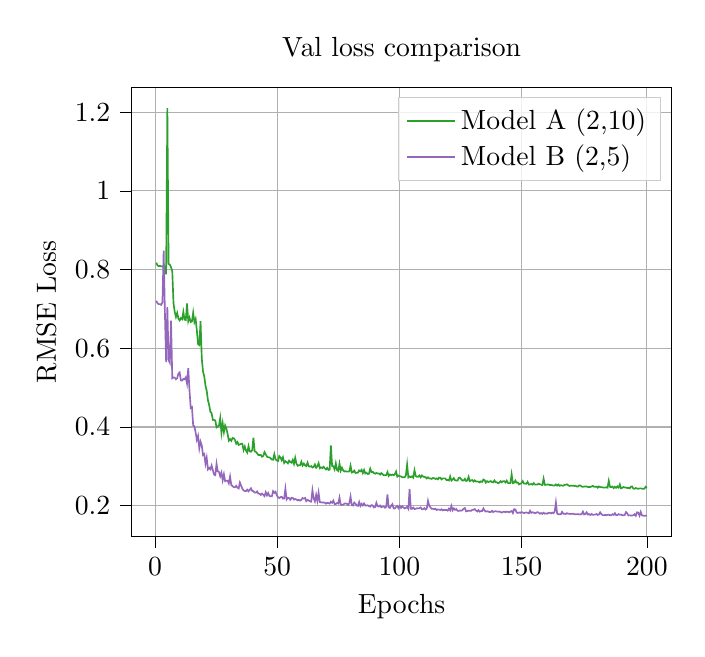
\begin{tikzpicture}

\definecolor{darkgray176}{RGB}{176,176,176}
\definecolor{forestgreen4416044}{RGB}{44,160,44}
\definecolor{lightgray204}{RGB}{204,204,204}
\definecolor{mediumpurple148103189}{RGB}{148,103,189}

\begin{axis}[
scaled ticks=false,
legend cell align={left},
legend style={fill opacity=0.8, draw opacity=1, text opacity=1, draw=lightgray204},
tick align=outside,
tick pos=left,
title={Val loss comparison},
x grid style={darkgray176},
xlabel={Epochs},
xmajorgrids,
xmin=-1479.1, xmax=32755.1,
xtick style={color=black},
xtick={0,7750,15500,23250,31200},
xticklabels={0,50,100,150,200},
y grid style={darkgray176},
ylabel={RMSE Loss},
ymajorgrids,
ymin=0.12233273088932, ymax=1.26202001273632,
ytick style={color=black}
]
\addplot [semithick, forestgreen4416044]
table {%
77 0.817664861679077
155 0.810476779937744
233 0.808972477912903
311 0.809321403503418
389 0.808443069458008
467 0.807960987091064
545 0.808243989944458
623 0.808139562606812
701 0.787868022918701
779 1.21021604537964
857 0.814702272415161
935 0.812561750411987
1013 0.805981516838074
1091 0.796039581298828
1169 0.71419095993042
1247 0.692407846450806
1325 0.679630041122437
1403 0.690068960189819
1481 0.675244569778442
1559 0.670684814453125
1637 0.676871418952942
1715 0.67397141456604
1793 0.692445755004883
1871 0.672709941864014
1949 0.671869039535522
2027 0.714231371879578
2105 0.668651342391968
2183 0.678156852722168
2261 0.666807174682617
2339 0.668517351150513
2417 0.690611362457275
2495 0.666260480880737
2573 0.674643993377686
2651 0.644995450973511
2729 0.610462188720703
2807 0.608117341995239
2885 0.668771982192993
2963 0.574352979660034
3041 0.540813446044922
3119 0.529028654098511
3197 0.505244970321655
3275 0.492183208465576
3353 0.468250155448914
3431 0.455799579620361
3509 0.438636898994446
3587 0.435343146324158
3665 0.417929887771606
3743 0.417998075485229
3821 0.41644012928009
3899 0.398920059204102
3977 0.401051998138428
4055 0.403836607933044
4133 0.422684073448181
4211 0.385217308998108
4289 0.409080505371094
4367 0.386908411979675
4445 0.403984308242798
4523 0.395946979522705
4601 0.382471680641174
4679 0.365227580070496
4757 0.369128465652466
4835 0.364861726760864
4913 0.371886730194092
4991 0.371472120285034
5069 0.366852164268494
5147 0.357492208480835
5225 0.361699104309082
5303 0.354348182678223
5381 0.355725169181824
5459 0.357224464416504
5537 0.357190608978271
5615 0.341452717781067
5693 0.350429058074951
5771 0.34000289440155
5849 0.334920763969421
5927 0.351287961006165
6005 0.33779764175415
6083 0.337132215499878
6161 0.340792059898376
6239 0.372683763504028
6317 0.337894439697266
6395 0.336796760559082
6473 0.333069562911987
6551 0.328731298446655
6629 0.328808069229126
6707 0.328718781471252
6785 0.324338793754578
6863 0.326165318489075
6941 0.336180210113525
7019 0.330429434776306
7097 0.324375987052917
7175 0.322977542877197
7253 0.322561144828796
7331 0.32046914100647
7409 0.317299365997314
7487 0.316826105117798
7565 0.330967307090759
7643 0.317682981491089
7721 0.314884424209595
7799 0.313461661338806
7877 0.325826168060303
7955 0.322529911994934
8033 0.315348625183105
8111 0.322973132133484
8189 0.308667302131653
8267 0.312951803207397
8345 0.310508489608765
8423 0.307454109191895
8501 0.31438422203064
8579 0.311030626296997
8657 0.309033632278442
8735 0.31635844707489
8813 0.306121587753296
8891 0.321569085121155
8969 0.306983351707458
9047 0.301435589790344
9125 0.303032159805298
9203 0.302685856819153
9281 0.311602115631104
9359 0.302019357681274
9437 0.306963324546814
9515 0.302188515663147
9593 0.300373554229736
9671 0.309417724609375
9749 0.299891710281372
9827 0.299054503440857
9905 0.300502777099609
9983 0.296937227249146
10061 0.298284769058228
10139 0.304667592048645
10217 0.296235203742981
10295 0.299856185913086
10373 0.308019876480103
10451 0.295146942138672
10529 0.29731011390686
10607 0.295497417449951
10685 0.298752546310425
10763 0.295133829116821
10841 0.292124032974243
10919 0.295958280563354
10997 0.290807604789734
11075 0.291584014892578
11153 0.353235602378845
11231 0.300697326660156
11309 0.300139784812927
11387 0.291935682296753
11465 0.307579159736633
11543 0.290753960609436
11621 0.288146734237671
11699 0.306883573532104
11777 0.288962960243225
11855 0.296632170677185
11933 0.289595127105713
12011 0.286815524101257
12089 0.28744900226593
12167 0.286450266838074
12245 0.286435127258301
12323 0.287057757377625
12401 0.301676034927368
12479 0.284043908119202
12557 0.285333275794983
12635 0.289117693901062
12713 0.283149480819702
12791 0.28326427936554
12869 0.283786296844482
12947 0.289608597755432
13025 0.287389039993286
13103 0.291091442108154
13181 0.28259539604187
13259 0.29084575176239
13337 0.28171181678772
13415 0.28371000289917
13493 0.280213952064514
13571 0.281321287155151
13649 0.294035196304321
13727 0.285523056983948
13805 0.285978078842163
13883 0.282775163650513
13961 0.281063199043274
14039 0.283217310905457
14117 0.281729102134705
14195 0.28192663192749
14273 0.278913021087646
14351 0.282656073570251
14429 0.280107259750366
14507 0.277080535888672
14585 0.277333498001099
14663 0.277456283569336
14741 0.285247325897217
14819 0.275621652603149
14897 0.2793790102005
14975 0.277329206466675
15053 0.278894901275635
15131 0.277351498603821
15209 0.279870748519897
15287 0.286622285842896
15365 0.273694634437561
15443 0.276440620422363
15521 0.274755001068115
15599 0.274191498756409
15677 0.272441029548645
15755 0.272176742553711
15833 0.272202610969543
15911 0.276858329772949
15989 0.304653882980347
16067 0.271635293960571
16145 0.274387359619141
16223 0.272396564483643
16301 0.274676203727722
16379 0.271180629730225
16457 0.289785861968994
16535 0.27541971206665
16613 0.273374080657959
16691 0.273280143737793
16769 0.276687383651733
16847 0.271892547607422
16925 0.276639223098755
17003 0.273638367652893
17081 0.273130655288696
17159 0.272330403327942
17237 0.269223213195801
17315 0.27192211151123
17393 0.269215106964111
17471 0.269020795822144
17549 0.267986536026001
17627 0.270293593406677
17705 0.269922971725464
17783 0.267749786376953
17861 0.269218444824219
17939 0.266875505447388
18017 0.271280288696289
18095 0.270978450775146
18173 0.266765356063843
18251 0.269158601760864
18329 0.269342064857483
18407 0.269200801849365
18485 0.265044569969177
18563 0.265523791313171
18641 0.263875722885132
18719 0.27432918548584
18797 0.263653755187988
18875 0.26632285118103
18953 0.269991874694824
19031 0.26442277431488
19109 0.26380443572998
19187 0.263558626174927
19265 0.2703697681427
19343 0.271199703216553
19421 0.266963601112366
19499 0.263847231864929
19577 0.263956189155579
19655 0.268267035484314
19733 0.262802958488464
19811 0.263822674751282
19889 0.273395657539368
19967 0.262372851371765
20045 0.264018058776855
20123 0.265174746513367
20201 0.261213660240173
20279 0.264276146888733
20357 0.261405825614929
20435 0.261351466178894
20513 0.260866641998291
20591 0.259069204330444
20669 0.261722683906555
20747 0.260394215583801
20825 0.266289710998535
20903 0.264716386795044
20981 0.25869607925415
21059 0.262226223945618
21137 0.259886026382446
21293 0.262465238571167
21371 0.259807467460632
21449 0.259145259857178
21527 0.263988614082336
21605 0.259507775306702
21683 0.259340643882751
21761 0.256866455078125
21839 0.258446097373962
21917 0.262205719947815
21995 0.25946056842804
22073 0.262107133865356
22151 0.262201428413391
22229 0.258838772773743
22307 0.263641715049744
22385 0.257822751998901
22463 0.256656885147095
22541 0.257414221763611
22619 0.279814720153809
22697 0.257223963737488
22775 0.258222579956055
22853 0.263801574707031
22931 0.258420467376709
23009 0.258842945098877
23087 0.253933072090149
23165 0.255602478981018
23243 0.257384181022644
23321 0.262344241142273
23399 0.256383538246155
23477 0.256071448326111
23555 0.255513310432434
23633 0.260440349578857
23711 0.253544688224792
23789 0.254104495048523
23867 0.255089521408081
23945 0.253378868103027
24023 0.257332682609558
24101 0.253361582756042
24179 0.253443598747253
24257 0.253935694694519
24335 0.255775451660156
24413 0.253952264785767
24491 0.253435254096985
24569 0.252254962921143
24647 0.268593192100525
24725 0.252785086631775
24803 0.252982497215271
24881 0.253695368766785
24959 0.254080772399902
25037 0.252195358276367
25115 0.25242280960083
25193 0.252100467681885
25271 0.251108527183533
25349 0.251136302947998
25427 0.254156947135925
25505 0.250955581665039
25583 0.253857612609863
25661 0.250282526016235
25739 0.252060890197754
25817 0.250932216644287
25895 0.250540614128113
25973 0.253004193305969
26051 0.253220677375793
26129 0.254208564758301
26207 0.251805782318115
26285 0.250096440315247
26363 0.250666379928589
26441 0.250829696655273
26519 0.250593304634094
26597 0.250014305114746
26675 0.250580430030823
26753 0.248533129692078
26831 0.248629331588745
26909 0.251675367355347
26987 0.250963568687439
27065 0.248432874679565
27143 0.247906565666199
27221 0.248576045036316
27299 0.248868584632874
27377 0.248812437057495
27455 0.247422456741333
27533 0.247582912445068
27611 0.247397184371948
27767 0.250246047973633
27845 0.248115539550781
27923 0.247939586639404
28001 0.248418807983398
28079 0.245715260505676
28157 0.248862862586975
28235 0.247295260429382
28313 0.247035384178162
28391 0.246442079544067
28469 0.245712757110596
28547 0.245737791061401
28625 0.246834516525269
28703 0.24559211730957
28781 0.263136148452759
28859 0.247809410095215
28937 0.247058868408203
29015 0.248512029647827
29093 0.244423985481262
29171 0.247967958450317
29249 0.245290398597717
29327 0.249018311500549
29405 0.245749711990356
29483 0.253933668136597
29561 0.243950724601746
29639 0.245309710502625
29717 0.247478246688843
29795 0.246039628982544
29873 0.245967864990234
29951 0.24480938911438
30029 0.245094656944275
30107 0.243952512741089
30185 0.248224020004272
30263 0.248708486557007
30341 0.243287920951843
30419 0.24299418926239
30497 0.244895458221436
30575 0.24355149269104
30653 0.242811441421509
30731 0.243844389915466
30809 0.243852376937866
30887 0.243149876594543
30965 0.242986083030701
31043 0.243143677711487
31121 0.247980356216431
31199 0.245247721672058
};
\addlegendentry{Model A (2,10)}
\addplot [semithick, mediumpurple148103189]
table {%
77 0.720663547515869
155 0.714586019515991
233 0.712193489074707
311 0.712183237075806
389 0.710559487342834
467 0.716590166091919
545 0.847949981689453
623 0.691815257072449
701 0.564696073532104
779 0.705025315284729
857 0.569925785064697
935 0.563602447509766
1013 0.670101284980774
1091 0.523851156234741
1169 0.525747776031494
1247 0.525474786758423
1325 0.521180510520935
1403 0.524107694625854
1481 0.535642862319946
1559 0.538802862167358
1637 0.518313765525818
1715 0.517933011054993
1793 0.521942615509033
1871 0.521209836006165
1949 0.526137351989746
2027 0.510377049446106
2105 0.549211263656616
2183 0.493334293365479
2261 0.448214173316956
2339 0.450559139251709
2417 0.404203176498413
2495 0.401160597801208
2573 0.38626492023468
2651 0.366923689842224
2729 0.377238750457764
2807 0.345525860786438
2885 0.362781643867493
2963 0.353190422058105
3041 0.328527450561523
3119 0.33126962184906
3197 0.306304335594177
3275 0.321839690208435
3353 0.292278051376343
3431 0.296190142631531
3509 0.292390823364258
3587 0.302237987518311
3665 0.28986394405365
3743 0.279147028923035
3821 0.277505993843079
3899 0.306552410125732
3977 0.287125706672668
4055 0.285808205604553
4133 0.274539113044739
4211 0.284061789512634
4289 0.264437317848206
4367 0.27960741519928
4445 0.262118339538574
4523 0.263541221618652
4601 0.263364195823669
4679 0.256513714790344
4757 0.273990988731384
4835 0.252574563026428
4913 0.249698281288147
4991 0.247003078460693
5069 0.246601343154907
5147 0.250362515449524
5225 0.245557904243469
5303 0.243707656860352
5381 0.258830904960632
5537 0.242895364761353
5615 0.238621950149536
5693 0.237289667129517
5771 0.236919522285461
5849 0.240662217140198
5927 0.236454010009766
6005 0.240103960037231
6083 0.244169950485229
6161 0.237426280975342
6239 0.236768245697021
6317 0.233256816864014
6395 0.232977628707886
6473 0.236210942268372
6551 0.230704307556152
6629 0.23020327091217
6707 0.227297425270081
6785 0.230805993080139
6863 0.227590560913086
6941 0.224169731140137
7019 0.234256505966187
7097 0.226062774658203
7175 0.23215389251709
7253 0.224554896354675
7331 0.223909974098206
7409 0.223760008811951
7487 0.23680591583252
7565 0.232579708099365
7643 0.235391616821289
7721 0.22661304473877
7799 0.221174240112305
7877 0.219267845153809
7955 0.221753120422363
8033 0.222527146339417
8111 0.217751383781433
8189 0.218132019042969
8267 0.243134140968323
8345 0.215770244598389
8423 0.220081329345703
8501 0.219274997711182
8579 0.214885711669922
8657 0.220079898834229
8735 0.21948504447937
8813 0.215313911437988
8891 0.216877102851868
8969 0.21560537815094
9047 0.213299632072449
9125 0.214911103248596
9203 0.212735056877136
9281 0.214770793914795
9359 0.219466686248779
9437 0.217876553535461
9515 0.219622850418091
9593 0.211329221725464
9671 0.214701414108276
9749 0.213033676147461
9827 0.210891604423523
9905 0.210192203521729
9983 0.239193677902222
10061 0.218197703361511
10139 0.21074640750885
10217 0.227540373802185
10295 0.212158799171448
10373 0.233051300048828
10451 0.208957672119141
10529 0.208586454391479
10607 0.207872033119202
10685 0.208078742027283
10763 0.20764422416687
10841 0.204961895942688
10919 0.207163214683533
10997 0.206516265869141
11075 0.205133438110352
11153 0.209931969642639
11231 0.207067608833313
11309 0.212607979774475
11387 0.204325914382935
11465 0.204198598861694
11543 0.206737637519836
11621 0.205393314361572
11699 0.22034740447998
11777 0.202061414718628
11855 0.202555894851685
11933 0.202040433883667
12011 0.205243945121765
12089 0.205745220184326
12167 0.20470118522644
12245 0.201573014259338
12323 0.206446170806885
12401 0.223132014274597
12479 0.201215505599976
12557 0.200291991233826
12635 0.207898139953613
12713 0.204994320869446
12791 0.200496673583984
12869 0.199295520782471
12947 0.209349870681763
13025 0.199070692062378
13103 0.204464554786682
13181 0.200539708137512
13259 0.205497145652771
13337 0.200425386428833
13415 0.200244545936584
13493 0.200941205024719
13571 0.198945879936218
13649 0.197392225265503
13727 0.201351404190063
13805 0.200437545776367
13883 0.195499897003174
13961 0.196535110473633
14039 0.207302808761597
14117 0.198211312294006
14195 0.197710514068604
14273 0.20030689239502
14351 0.19591748714447
14429 0.197264432907104
14507 0.1978679895401
14585 0.19472062587738
14663 0.197254776954651
14741 0.228304743766785
14819 0.195481300354004
14897 0.194243431091309
14975 0.199690818786621
15053 0.20378589630127
15131 0.193080544471741
15209 0.192768335342407
15287 0.196632862091064
15365 0.199046969413757
15443 0.193581461906433
15521 0.199118256568909
15599 0.194183707237244
15677 0.198325872421265
15755 0.195496320724487
15833 0.193098425865173
15911 0.194101452827454
15989 0.197414994239807
16067 0.191949248313904
16145 0.242612838745117
16223 0.192159295082092
16301 0.191947221755981
16379 0.195167303085327
16457 0.191385746002197
16535 0.191903948783875
16613 0.193448185920715
16691 0.192842960357666
16769 0.193737626075745
16847 0.195410013198853
16925 0.19087541103363
17003 0.191103935241699
17081 0.193611979484558
17159 0.190101385116577
17237 0.192493677139282
17315 0.212269902229309
17393 0.199789762496948
17549 0.191774249076843
17627 0.191968441009521
17705 0.191141486167908
17783 0.19200611114502
17861 0.189013481140137
17939 0.190235376358032
18095 0.189046621322632
18173 0.1908278465271
18251 0.187855839729309
18329 0.189326405525208
18407 0.188784956932068
18485 0.189098834991455
18563 0.187267899513245
18641 0.192423343658447
18719 0.18808126449585
18797 0.199304103851318
18875 0.18820595741272
18953 0.193197727203369
19031 0.189382553100586
19109 0.191338062286377
19187 0.18691885471344
19265 0.186583399772644
19343 0.187700271606445
19421 0.187110185623169
19499 0.188506126403809
19577 0.192346811294556
19655 0.193882346153259
19733 0.185503005981445
19811 0.18621563911438
19889 0.18708872795105
20045 0.186768531799316
20123 0.189706206321716
20201 0.189590454101562
20279 0.191205859184265
20357 0.18775475025177
20435 0.185319066047668
20513 0.188611507415771
20591 0.184644460678101
20669 0.186187744140625
20747 0.186458230018616
20825 0.192888021469116
20903 0.187733292579651
20981 0.184862375259399
21059 0.185800671577454
21137 0.184997797012329
21215 0.183643579483032
21293 0.183959245681763
21371 0.186948657035828
21449 0.183557152748108
21527 0.185314536094666
21605 0.185765862464905
21761 0.184510946273804
21839 0.184943079948425
21917 0.183830738067627
21995 0.182361125946045
22073 0.184063911437988
22151 0.184707880020142
22229 0.183201432228088
22307 0.184631586074829
22385 0.184431433677673
22463 0.18302309513092
22541 0.185139417648315
22619 0.186387419700623
22697 0.181075215339661
22775 0.19075345993042
22853 0.190507650375366
22931 0.182946681976318
23009 0.181249737739563
23087 0.182727456092834
23165 0.181663632392883
23243 0.183599948883057
23321 0.182767510414124
23399 0.181137919425964
23477 0.182000517845154
23555 0.182491540908813
23633 0.181938886642456
23711 0.18052077293396
23789 0.187005877494812
23867 0.181593418121338
23945 0.183211088180542
24023 0.182280421257019
24101 0.180620551109314
24179 0.181951522827148
24257 0.183434963226318
24335 0.181959748268127
24413 0.17946183681488
24491 0.181104779243469
24569 0.179097175598145
24647 0.181948184967041
24725 0.179523468017578
24803 0.180326223373413
24881 0.179579019546509
24959 0.181986689567566
25037 0.18166720867157
25115 0.180296182632446
25193 0.18239414691925
25271 0.180845499038696
25349 0.184744477272034
25427 0.208020925521851
25505 0.179789304733276
25583 0.178001880645752
25661 0.178200483322144
25739 0.177942514419556
25817 0.184017539024353
25895 0.179326057434082
25973 0.17952024936676
26051 0.178835511207581
26129 0.180870175361633
26207 0.179261207580566
26285 0.179655075073242
26363 0.17871105670929
26441 0.17938506603241
26519 0.179546475410461
26597 0.178095817565918
26675 0.178184151649475
26753 0.178061127662659
26831 0.178580045700073
26909 0.177585363388062
26987 0.178196907043457
27065 0.178269505500793
27143 0.184645652770996
27221 0.177530169487
27299 0.178929805755615
27377 0.182997226715088
27455 0.177355289459229
27533 0.178629636764526
27611 0.17619800567627
27689 0.178887844085693
27767 0.176697611808777
27845 0.176940441131592
27923 0.177311301231384
28001 0.178773641586304
28079 0.176333546638489
28157 0.177432537078857
28235 0.183019876480103
28313 0.17855441570282
28391 0.175983428955078
28469 0.175367116928101
28547 0.176577925682068
28625 0.175767779350281
28703 0.176540374755859
28781 0.176788806915283
28859 0.175861954689026
28937 0.175482034683228
29015 0.178200364112854
29093 0.176411271095276
29171 0.180875182151794
29249 0.175769090652466
29327 0.175926089286804
29405 0.178342819213867
29483 0.177014827728271
29561 0.177253007888794
29639 0.175495505332947
29717 0.175577521324158
29795 0.176311731338501
29873 0.18372917175293
29951 0.180235981941223
30029 0.175057172775269
30107 0.175400018692017
30185 0.174803018569946
30263 0.174801826477051
30341 0.175623536109924
30419 0.178174257278442
30497 0.174136638641357
30575 0.183080673217773
30653 0.182068347930908
30731 0.174509286880493
30809 0.184078812599182
30887 0.175265550613403
30965 0.17454195022583
31043 0.174182534217834
31121 0.174708724021912
31199 0.174251794815063
};
\addlegendentry{Model B (2,5)}
\end{axis}

\end{tikzpicture}

	}
\end{figure}

	\begin{figure}
	\centering
	\resizebox{0.95\textwidth}{!}{
		% This file was created with matplot2tikz v0.4.0.
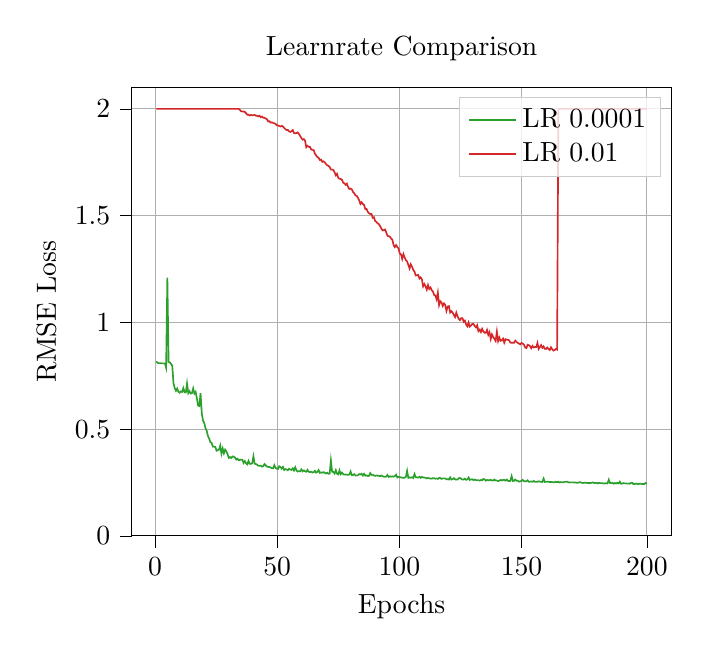
\begin{tikzpicture}

\definecolor{crimson2143940}{RGB}{214,39,40}
\definecolor{darkgray176}{RGB}{176,176,176}
\definecolor{forestgreen4416044}{RGB}{44,160,44}
\definecolor{lightgray204}{RGB}{204,204,204}

\begin{axis}[
scaled ticks=false,
legend cell align={left},
legend style={fill opacity=0.8, draw opacity=1, text opacity=1, draw=lightgray204},
tick align=outside,
tick pos=left,
title={Learnrate Comparison},
x grid style={darkgray176},
xlabel={Epochs},
xmajorgrids,
xmin=-1479.1, xmax=32755.1,
xtick style={color=black},
xtick={0,7750,15500,23250,31200},
xticklabels={0,50,100,150,200},
y grid style={darkgray176},
ylabel={RMSE Loss},
ymajorgrids,
ymin=0, ymax=2.1,
ytick style={color=black}
]
\addplot [semithick, forestgreen4416044]
table {%
77 0.817664861679077
155 0.810476779937744
233 0.808972477912903
311 0.809321403503418
389 0.808443069458008
467 0.807960987091064
545 0.808243989944458
623 0.808139562606812
701 0.787868022918701
779 1.21021604537964
857 0.814702272415161
935 0.812561750411987
1013 0.805981516838074
1091 0.796039581298828
1169 0.71419095993042
1247 0.692407846450806
1325 0.679630041122437
1403 0.690068960189819
1481 0.675244569778442
1559 0.670684814453125
1637 0.676871418952942
1715 0.67397141456604
1793 0.692445755004883
1871 0.672709941864014
1949 0.671869039535522
2027 0.714231371879578
2105 0.668651342391968
2183 0.678156852722168
2261 0.666807174682617
2339 0.668517351150513
2417 0.690611362457275
2495 0.666260480880737
2573 0.674643993377686
2651 0.644995450973511
2729 0.610462188720703
2807 0.608117341995239
2885 0.668771982192993
2963 0.574352979660034
3041 0.540813446044922
3119 0.529028654098511
3197 0.505244970321655
3275 0.492183208465576
3353 0.468250155448914
3431 0.455799579620361
3509 0.438636898994446
3587 0.435343146324158
3665 0.417929887771606
3743 0.417998075485229
3821 0.41644012928009
3899 0.398920059204102
3977 0.401051998138428
4055 0.403836607933044
4133 0.422684073448181
4211 0.385217308998108
4289 0.409080505371094
4367 0.386908411979675
4445 0.403984308242798
4523 0.395946979522705
4601 0.382471680641174
4679 0.365227580070496
4757 0.369128465652466
4835 0.364861726760864
4913 0.371886730194092
4991 0.371472120285034
5069 0.366852164268494
5147 0.357492208480835
5225 0.361699104309082
5303 0.354348182678223
5459 0.357224464416504
5537 0.357190608978271
5615 0.341452717781067
5693 0.350429058074951
5771 0.34000289440155
5849 0.334920763969421
5927 0.351287961006165
6005 0.33779764175415
6083 0.337132215499878
6161 0.340792059898376
6239 0.372683763504028
6317 0.337894439697266
6395 0.336796760559082
6473 0.333069562911987
6551 0.328731298446655
6707 0.328718781471252
6785 0.324338793754578
6863 0.326165318489075
6941 0.336180210113525
7019 0.330429434776306
7097 0.324375987052917
7175 0.322977542877197
7253 0.322561144828796
7331 0.32046914100647
7409 0.317299365997314
7487 0.316826105117798
7565 0.330967307090759
7643 0.317682981491089
7721 0.314884424209595
7799 0.313461661338806
7877 0.325826168060303
7955 0.322529911994934
8033 0.315348625183105
8111 0.322973132133484
8189 0.308667302131653
8267 0.312951803207397
8345 0.310508489608765
8423 0.307454109191895
8501 0.31438422203064
8579 0.311030626296997
8657 0.309033632278442
8735 0.31635844707489
8813 0.306121587753296
8891 0.321569085121155
8969 0.306983351707458
9047 0.301435589790344
9125 0.303032159805298
9203 0.302685856819153
9281 0.311602115631104
9359 0.302019357681274
9437 0.306963324546814
9515 0.302188515663147
9593 0.300373554229736
9671 0.309417724609375
9749 0.299891710281372
9827 0.299054503440857
9905 0.300502777099609
9983 0.296937227249146
10061 0.298284769058228
10139 0.304667592048645
10217 0.296235203742981
10295 0.299856185913086
10373 0.308019876480103
10451 0.295146942138672
10529 0.29731011390686
10607 0.295497417449951
10685 0.298752546310425
10763 0.295133829116821
10841 0.292124032974243
10919 0.295958280563354
10997 0.290807604789734
11075 0.291584014892578
11153 0.353235602378845
11231 0.300697326660156
11309 0.300139784812927
11387 0.291935682296753
11465 0.307579159736633
11543 0.290753960609436
11621 0.288146734237671
11699 0.306883573532104
11777 0.288962960243225
11855 0.296632170677185
11933 0.289595127105713
12011 0.286815524101257
12089 0.28744900226593
12167 0.286450266838074
12245 0.286435127258301
12323 0.287057757377625
12401 0.301676034927368
12479 0.284043908119202
12557 0.285333275794983
12635 0.289117693901062
12713 0.283149480819702
12791 0.28326427936554
12869 0.283786296844482
12947 0.289608597755432
13025 0.287389039993286
13103 0.291091442108154
13181 0.28259539604187
13259 0.29084575176239
13337 0.28171181678772
13415 0.28371000289917
13493 0.280213952064514
13571 0.281321287155151
13649 0.294035196304321
13727 0.285523056983948
13805 0.285978078842163
13883 0.282775163650513
13961 0.281063199043274
14039 0.283217310905457
14117 0.281729102134705
14195 0.28192663192749
14273 0.278913021087646
14351 0.282656073570251
14429 0.280107259750366
14507 0.277080535888672
14663 0.277456283569336
14741 0.285247325897217
14819 0.275621652603149
14897 0.2793790102005
14975 0.277329206466675
15053 0.278894901275635
15131 0.277351498603821
15209 0.279870748519897
15287 0.286622285842896
15365 0.273694634437561
15443 0.276440620422363
15521 0.274755001068115
15599 0.274191498756409
15677 0.272441029548645
15755 0.272176742553711
15833 0.272202610969543
15911 0.276858329772949
15989 0.304653882980347
16067 0.271635293960571
16145 0.274387359619141
16223 0.272396564483643
16301 0.274676203727722
16379 0.271180629730225
16457 0.289785861968994
16535 0.27541971206665
16613 0.273374080657959
16691 0.273280143737793
16769 0.276687383651733
16847 0.271892547607422
16925 0.276639223098755
17003 0.273638367652893
17081 0.273130655288696
17159 0.272330403327942
17237 0.269223213195801
17315 0.27192211151123
17393 0.269215106964111
17471 0.269020795822144
17549 0.267986536026001
17627 0.270293593406677
17705 0.269922971725464
17783 0.267749786376953
17861 0.269218444824219
17939 0.266875505447388
18017 0.271280288696289
18095 0.270978450775146
18173 0.266765356063843
18251 0.269158601760864
18329 0.269342064857483
18407 0.269200801849365
18485 0.265044569969177
18563 0.265523791313171
18641 0.263875722885132
18719 0.27432918548584
18797 0.263653755187988
18875 0.26632285118103
18953 0.269991874694824
19031 0.26442277431488
19109 0.26380443572998
19187 0.263558626174927
19265 0.2703697681427
19343 0.271199703216553
19421 0.266963601112366
19499 0.263847231864929
19577 0.263956189155579
19655 0.268267035484314
19733 0.262802958488464
19811 0.263822674751282
19889 0.273395657539368
19967 0.262372851371765
20045 0.264018058776855
20123 0.265174746513367
20201 0.261213660240173
20279 0.264276146888733
20357 0.261405825614929
20435 0.261351466178894
20513 0.260866641998291
20591 0.259069204330444
20669 0.261722683906555
20747 0.260394215583801
20825 0.266289710998535
20903 0.264716386795044
20981 0.25869607925415
21059 0.262226223945618
21137 0.259886026382446
21293 0.262465238571167
21371 0.259807467460632
21449 0.259145259857178
21527 0.263988614082336
21605 0.259507775306702
21683 0.259340643882751
21761 0.256866455078125
21839 0.258446097373962
21917 0.262205719947815
21995 0.25946056842804
22073 0.262107133865356
22151 0.262201428413391
22229 0.258838772773743
22307 0.263641715049744
22385 0.257822751998901
22463 0.256656885147095
22541 0.257414221763611
22619 0.279814720153809
22697 0.257223963737488
22775 0.258222579956055
22853 0.263801574707031
22931 0.258420467376709
23009 0.258842945098877
23087 0.253933072090149
23243 0.257384181022644
23321 0.262344241142273
23399 0.256383538246155
23477 0.256071448326111
23555 0.255513310432434
23633 0.260440349578857
23711 0.253544688224792
23789 0.254104495048523
23867 0.255089521408081
23945 0.253378868103027
24023 0.257332682609558
24101 0.253361582756042
24179 0.253443598747253
24257 0.253935694694519
24335 0.255775451660156
24413 0.253952264785767
24491 0.253435254096985
24569 0.252254962921143
24647 0.268593192100525
24725 0.252785086631775
24803 0.252982497215271
24881 0.253695368766785
24959 0.254080772399902
25037 0.252195358276367
25115 0.25242280960083
25193 0.252100467681885
25271 0.251108527183533
25349 0.251136302947998
25427 0.254156947135925
25505 0.250955581665039
25583 0.253857612609863
25661 0.250282526016235
25739 0.252060890197754
25817 0.250932216644287
25895 0.250540614128113
25973 0.253004193305969
26051 0.253220677375793
26129 0.254208564758301
26207 0.251805782318115
26285 0.250096440315247
26363 0.250666379928589
26441 0.250829696655273
26519 0.250593304634094
26597 0.250014305114746
26675 0.250580430030823
26753 0.248533129692078
26831 0.248629331588745
26909 0.251675367355347
26987 0.250963568687439
27065 0.248432874679565
27143 0.247906565666199
27221 0.248576045036316
27299 0.248868584632874
27377 0.248812437057495
27455 0.247422456741333
27533 0.247582912445068
27611 0.247397184371948
27767 0.250246047973633
27845 0.248115539550781
27923 0.247939586639404
28001 0.248418807983398
28079 0.245715260505676
28157 0.248862862586975
28235 0.247295260429382
28313 0.247035384178162
28469 0.245712757110596
28547 0.245737791061401
28625 0.246834516525269
28703 0.24559211730957
28781 0.263136148452759
28859 0.247809410095215
28937 0.247058868408203
29015 0.248512029647827
29093 0.244423985481262
29171 0.247967958450317
29249 0.245290398597717
29327 0.249018311500549
29405 0.245749711990356
29483 0.253933668136597
29561 0.243950724601746
29639 0.245309710502625
29717 0.247478246688843
29795 0.246039628982544
29873 0.245967864990234
29951 0.24480938911438
30029 0.245094656944275
30107 0.243952512741089
30185 0.248224020004272
30263 0.248708486557007
30341 0.243287920951843
30419 0.24299418926239
30497 0.244895458221436
30575 0.24355149269104
30653 0.242811441421509
30731 0.243844389915466
30809 0.243852376937866
30887 0.243149876594543
30965 0.242986083030701
31043 0.243143677711487
31121 0.247980356216431
31199 0.245247721672058
};
\addlegendentry{LR 0.0001}
\addplot [semithick, crimson2143940]
table {%
77 2
5303 2
5381 1.99543023109436
5459 1.98865461349487
5615 1.98759818077087
5693 1.98584914207458
5771 1.98023903369904
5849 1.97246313095093
5927 1.97335839271545
6005 1.96927690505981
6083 1.97151815891266
6161 1.970050573349
6317 1.97147834300995
6395 1.96845412254333
6473 1.96756219863892
6551 1.96499276161194
6629 1.96809220314026
6707 1.96151733398438
6785 1.96391677856445
6863 1.95879769325256
6941 1.95829260349274
7019 1.95506238937378
7097 1.95145010948181
7175 1.94123792648315
7253 1.94230985641479
7331 1.93594086170197
7409 1.93706047534943
7487 1.93448317050934
7565 1.9324164390564
7643 1.92989373207092
7721 1.92367994785309
7799 1.92213082313538
7877 1.92010962963104
7955 1.9175968170166
8033 1.92040419578552
8111 1.91780364513397
8189 1.91091322898865
8267 1.90512275695801
8345 1.90115332603455
8423 1.90172898769379
8501 1.89460325241089
8579 1.89225554466248
8657 1.89520180225372
8735 1.90063989162445
8813 1.88758409023285
8891 1.88516402244568
8969 1.88728249073029
9047 1.89002633094788
9125 1.88209426403046
9203 1.87341070175171
9281 1.86438798904419
9359 1.85595643520355
9437 1.85837984085083
9515 1.85084784030914
9593 1.82068693637848
9671 1.82722008228302
9749 1.82227599620819
9827 1.8215639591217
9905 1.80974793434143
10061 1.80676329135895
10139 1.79027771949768
10217 1.78172707557678
10295 1.77460896968842
10373 1.77086079120636
10451 1.76080548763275
10529 1.76233291625977
10607 1.7518562078476
10685 1.75455808639526
10763 1.74977445602417
10841 1.74212455749512
10919 1.73524117469788
10997 1.73390471935272
11075 1.72760438919067
11153 1.71561706066132
11231 1.71549582481384
11309 1.71365964412689
11387 1.70322287082672
11465 1.6889773607254
11543 1.69622826576233
11621 1.67697894573212
11699 1.67283129692078
11777 1.67169260978699
11855 1.66836285591125
11933 1.65451216697693
12011 1.65162193775177
12089 1.64456355571747
12167 1.64998054504395
12245 1.63389253616333
12323 1.62480854988098
12401 1.62691497802734
12479 1.62353003025055
12557 1.6109231710434
12635 1.60534834861755
12713 1.59475457668304
12791 1.59283006191254
12869 1.58415961265564
12947 1.57178473472595
13025 1.55492854118347
13103 1.56273698806763
13181 1.55442023277283
13259 1.55018031597137
13337 1.53101098537445
13415 1.53123986721039
13493 1.51793360710144
13571 1.51121306419373
13649 1.50798177719116
13727 1.50839197635651
13805 1.4902606010437
13883 1.49263215065002
13961 1.47464084625244
14039 1.47118008136749
14117 1.46372938156128
14195 1.46059429645538
14273 1.45117974281311
14429 1.43052816390991
14507 1.43240344524384
14585 1.43527948856354
14663 1.4219206571579
14741 1.40580749511719
14819 1.40386343002319
14897 1.40138328075409
14975 1.39314711093903
15053 1.38739573955536
15131 1.36198770999908
15209 1.35266005992889
15287 1.36233460903168
15365 1.35342395305634
15443 1.34677577018738
15521 1.322678565979
15599 1.31885361671448
15677 1.29711306095123
15755 1.31971311569214
15833 1.3044730424881
15911 1.29129993915558
15989 1.28614091873169
16067 1.26934337615967
16145 1.25224995613098
16223 1.27239644527435
16301 1.26099848747253
16379 1.24550902843475
16457 1.23811256885529
16535 1.21981728076935
16613 1.22063255310059
16691 1.22260129451752
16769 1.20540189743042
16847 1.21103262901306
16925 1.20235562324524
17003 1.16878759860992
17081 1.17993032932281
17159 1.16913175582886
17237 1.15338504314423
17315 1.17491400241852
17393 1.15650832653046
17471 1.16345834732056
17549 1.1513192653656
17627 1.14462208747864
17705 1.12847685813904
17783 1.12564134597778
17861 1.1078690290451
17939 1.13951337337494
18017 1.08076882362366
18095 1.09907579421997
18173 1.09320306777954
18251 1.07678020000458
18329 1.0889595746994
18407 1.08194649219513
18485 1.05384314060211
18563 1.07446384429932
18641 1.07596385478973
18719 1.046431183815
18797 1.05292081832886
18875 1.04627180099487
18953 1.03462791442871
19031 1.02512216567993
19109 1.04600095748901
19187 1.02886724472046
19265 1.01642060279846
19343 1.01075124740601
19421 1.02017736434937
19499 1.01987671852112
19577 1.00247478485107
19655 1.00816738605499
19733 0.989968776702881
19811 0.981695413589478
19889 0.999432563781738
19967 0.97973895072937
20045 0.985476732254028
20123 0.993234515190125
20201 0.992460966110229
20279 0.983298182487488
20357 0.976655244827271
20435 0.986316204071045
20513 0.958983659744263
20591 0.96589457988739
20669 0.95433521270752
20747 0.96992564201355
20825 0.957933187484741
20903 0.951143980026245
20981 0.951233863830566
21059 0.964608907699585
21137 0.941456317901611
21215 0.954050779342651
21293 0.922453999519348
21371 0.943914890289307
21449 0.931177139282227
21527 0.923144102096558
21605 0.913157224655151
21683 0.956724882125854
21761 0.912326097488403
21839 0.928631067276001
21917 0.913403749465942
21995 0.916110157966614
22073 0.924084544181824
22151 0.90514349937439
22229 0.921234369277954
22307 0.918914794921875
22385 0.918835759162903
22463 0.915562510490417
22541 0.905173540115356
22619 0.904273271560669
22697 0.904569864273071
22775 0.904672741889954
22853 0.915003895759583
22931 0.909216642379761
23009 0.903669834136963
23087 0.901153445243835
23165 0.897149562835693
23243 0.903702259063721
23321 0.900866508483887
23399 0.895714521408081
23477 0.88292932510376
23555 0.879832148551941
23633 0.895259976387024
23711 0.893388748168945
23789 0.888480424880981
23867 0.879018068313599
23945 0.889875173568726
24023 0.882734179496765
24101 0.884774923324585
24179 0.884295701980591
24257 0.903647303581238
24335 0.87555718421936
24413 0.885122895240784
24491 0.893695831298828
24569 0.881012797355652
24647 0.887791752815247
24725 0.876229524612427
24803 0.875541925430298
24881 0.8824063539505
24959 0.875582218170166
25037 0.870578527450562
25115 0.8832106590271
25193 0.87453818321228
25271 0.868051290512085
25349 0.870121240615845
25427 0.875908017158508
25505 0.872875928878784
25583 2
31199 2
};
\addlegendentry{LR 0.01}
\end{axis}

\end{tikzpicture}

		% This file was created with matplot2tikz v0.4.0.
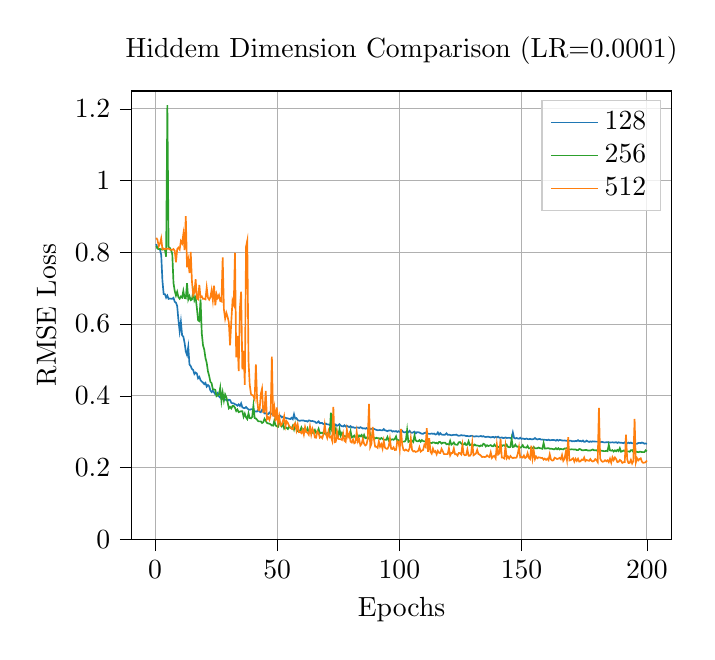
\begin{tikzpicture}

\definecolor{darkgray176}{RGB}{176,176,176}
\definecolor{darkorange25512714}{RGB}{255,127,14}
\definecolor{forestgreen4416044}{RGB}{44,160,44}
\definecolor{lightgray204}{RGB}{204,204,204}
\definecolor{steelblue31119180}{RGB}{31,119,180}

\begin{axis}[
scaled ticks=false,
legend cell align={left},
legend style={fill opacity=0.8, draw opacity=1, text opacity=1, draw=lightgray204},
tick align=outside,
tick pos=left,
title={Hiddem Dimension Comparison (LR=0.0001)},
x grid style={darkgray176},
xlabel={Epochs},
xmajorgrids,
xmin=-1479.1, xmax=32755.1,
xtick style={color=black},
xtick={0,7750,15500,23250,31200},
xticklabels={0,50,100,150,200},
y grid style={darkgray176},
ylabel={RMSE Loss},
ymajorgrids,
ymin=0, ymax=1.25,
ytick style={color=black}
]
\addplot [semithick, steelblue31119180]
table {%
	77 0.823244333267212
	155 0.810923457145691
	233 0.809678912162781
	311 0.807851791381836
	389 0.793118834495544
	467 0.720842123031616
	545 0.683714866638184
	623 0.683571696281433
	701 0.673680067062378
	779 0.679588556289673
	857 0.670158743858337
	935 0.671225309371948
	1013 0.670679688453674
	1091 0.67062520980835
	1169 0.673257827758789
	1247 0.662304162979126
	1325 0.659829378128052
	1403 0.650222659111023
	1481 0.611560940742493
	1559 0.580204129219055
	1637 0.606862783432007
	1715 0.568431615829468
	1793 0.565324783325195
	1871 0.548252582550049
	1949 0.523439049720764
	2027 0.513779640197754
	2105 0.536531925201416
	2183 0.487249612808228
	2261 0.482752323150635
	2339 0.474714756011963
	2417 0.472067594528198
	2495 0.460716009140015
	2573 0.464881658554077
	2651 0.462408781051636
	2729 0.448829650878906
	2807 0.452791213989258
	2885 0.443522930145264
	2963 0.439743638038635
	3041 0.43694531917572
	3119 0.43245804309845
	3197 0.436127781867981
	3275 0.425488114356995
	3353 0.430047512054443
	3431 0.426895976066589
	3509 0.414905309677124
	3587 0.410344123840332
	3665 0.414306402206421
	3743 0.409626841545105
	3821 0.404414892196655
	3899 0.40488076210022
	3977 0.408333897590637
	4055 0.398009300231934
	4133 0.394547343254089
	4211 0.397850155830383
	4289 0.392553567886353
	4367 0.391542196273804
	4445 0.389134049415588
	4523 0.389074802398682
	4601 0.385660648345947
	4679 0.38921320438385
	4757 0.387972116470337
	4835 0.380612254142761
	4913 0.379112482070923
	4991 0.379015922546387
	5069 0.376535892486572
	5147 0.37514054775238
	5225 0.372457385063171
	5303 0.376158714294434
	5381 0.371665000915527
	5459 0.379019975662231
	5537 0.367748737335205
	5615 0.366181135177612
	5693 0.365472555160522
	5771 0.368818640708923
	5849 0.36485481262207
	5927 0.361990451812744
	6005 0.361122369766235
	6083 0.362309813499451
	6161 0.362403035163879
	6239 0.361322164535522
	6317 0.356767892837524
	6395 0.355867624282837
	6473 0.356350421905518
	6551 0.362553000450134
	6629 0.355949759483337
	6707 0.354128479957581
	6785 0.360849380493164
	6863 0.357438445091248
	6941 0.350870847702026
	7019 0.351462244987488
	7097 0.347939014434814
	7175 0.348957180976868
	7253 0.353357791900635
	7331 0.349750876426697
	7409 0.350595831871033
	7487 0.345902562141418
	7565 0.344219088554382
	7643 0.343443512916565
	7721 0.343321919441223
	7799 0.343916654586792
	7877 0.343722462654114
	7955 0.344620943069458
	8033 0.339967727661133
	8111 0.341961622238159
	8189 0.338783502578735
	8267 0.338654398918152
	8345 0.337475180625916
	8423 0.337168216705322
	8501 0.33600902557373
	8579 0.335222125053406
	8657 0.338611006736755
	8735 0.334934830665588
	8813 0.348727703094482
	8891 0.336330771446228
	8969 0.337712526321411
	9047 0.332253813743591
	9125 0.330737709999084
	9203 0.330475449562073
	9281 0.33153223991394
	9437 0.330914974212646
	9515 0.329367637634277
	9593 0.32970929145813
	9671 0.327893853187561
	9749 0.331417083740234
	9827 0.330828189849854
	9905 0.329257369041443
	9983 0.329781293869019
	10061 0.328652381896973
	10139 0.327881217002869
	10217 0.324357271194458
	10295 0.325494050979614
	10373 0.328838109970093
	10451 0.323470711708069
	10529 0.32438588142395
	10607 0.324111223220825
	10685 0.321066975593567
	10763 0.320462346076965
	10841 0.322427272796631
	10919 0.320261240005493
	10997 0.320265054702759
	11075 0.31879997253418
	11153 0.319420337677002
	11231 0.321774005889893
	11309 0.318264245986938
	11387 0.31716251373291
	11465 0.320024251937866
	11543 0.316459536552429
	11621 0.317841649055481
	11699 0.32092559337616
	11777 0.316833853721619
	11855 0.315162897109985
	11933 0.314655065536499
	12011 0.317806601524353
	12089 0.314450263977051
	12167 0.316713094711304
	12245 0.314261674880981
	12323 0.312469363212585
	12401 0.315545439720154
	12479 0.311714649200439
	12557 0.312770366668701
	12635 0.311119914054871
	12713 0.311035752296448
	12791 0.311498761177063
	12869 0.311650991439819
	12947 0.310278058052063
	13025 0.312493205070496
	13103 0.310859203338623
	13181 0.308799147605896
	13259 0.309572696685791
	13337 0.308375477790833
	13415 0.310170650482178
	13493 0.307314872741699
	13571 0.306268930435181
	13649 0.307212948799133
	13727 0.307991027832031
	13805 0.307663440704346
	13883 0.308021545410156
	13961 0.306301474571228
	14039 0.304998993873596
	14117 0.304082870483398
	14195 0.304299354553223
	14273 0.304641008377075
	14351 0.303691148757935
	14429 0.303688168525696
	14507 0.307368755340576
	14585 0.30361270904541
	14663 0.302977442741394
	14741 0.301372528076172
	14819 0.303161144256592
	14975 0.303657174110413
	15053 0.300204396247864
	15131 0.301537871360779
	15209 0.300402283668518
	15287 0.301698207855225
	15365 0.299181222915649
	15443 0.301314115524292
	15521 0.299442887306213
	15599 0.298901796340942
	15677 0.30227267742157
	15755 0.298697352409363
	15833 0.297991871833801
	15911 0.298927545547485
	15989 0.298499226570129
	16067 0.298187732696533
	16145 0.302335262298584
	16223 0.297933101654053
	16301 0.296787023544312
	16379 0.298194527626038
	16457 0.300183296203613
	16535 0.295301556587219
	16613 0.298590421676636
	16691 0.298442363739014
	16769 0.297739267349243
	16847 0.295708179473877
	16925 0.294268608093262
	17003 0.293936848640442
	17081 0.296270489692688
	17159 0.297314882278442
	17237 0.294184565544128
	17315 0.294680833816528
	17393 0.293816328048706
	17471 0.293971657752991
	17549 0.294866800308228
	17627 0.294035673141479
	17705 0.29466724395752
	17783 0.292120933532715
	17861 0.292998790740967
	17939 0.298105597496033
	18017 0.291807174682617
	18095 0.295870661735535
	18173 0.292076349258423
	18251 0.291488647460938
	18329 0.291232109069824
	18407 0.29178786277771
	18485 0.295592784881592
	18563 0.291299223899841
	18641 0.291789770126343
	18797 0.289938569068909
	18875 0.290672540664673
	18953 0.29128110408783
	19031 0.290949106216431
	19109 0.291817426681519
	19187 0.28957736492157
	19265 0.288683772087097
	19343 0.289172887802124
	19421 0.290418386459351
	19499 0.289542675018311
	19577 0.289605975151062
	19655 0.289113998413086
	19733 0.287867546081543
	19811 0.287865877151489
	19889 0.287442564964294
	19967 0.287259459495544
	20045 0.288532257080078
	20123 0.288091421127319
	20201 0.286683082580566
	20279 0.286196708679199
	20357 0.287512183189392
	20513 0.286699771881104
	20591 0.286841869354248
	20669 0.28800630569458
	20747 0.286270499229431
	20825 0.287586331367493
	20903 0.285749673843384
	20981 0.285162925720215
	21059 0.285818696022034
	21137 0.285963296890259
	21215 0.285041570663452
	21293 0.283973693847656
	21371 0.284909009933472
	21449 0.28549587726593
	21527 0.283396124839783
	21605 0.285807490348816
	21683 0.283632397651672
	21761 0.286231994628906
	21839 0.28325879573822
	21917 0.282896041870117
	21995 0.284018635749817
	22073 0.282421231269836
	22151 0.282571792602539
	22229 0.284016728401184
	22307 0.282438158988953
	22463 0.282951235771179
	22619 0.281750679016113
	22697 0.297805309295654
	22775 0.28252911567688
	22853 0.281017661094666
	22931 0.282618403434753
	23009 0.280905365943909
	23087 0.280309915542603
	23165 0.283118486404419
	23243 0.279898643493652
	23321 0.280893564224243
	23477 0.279268980026245
	23555 0.280965089797974
	23633 0.279483795166016
	23711 0.278979182243347
	23789 0.280040860176086
	23867 0.278848767280579
	23945 0.278720617294312
	24023 0.279592275619507
	24101 0.282448410987854
	24179 0.279441595077515
	24257 0.278324365615845
	24335 0.279367089271545
	24413 0.279906272888184
	24491 0.277871489524841
	24569 0.277992725372314
	24647 0.277304649353027
	24725 0.277334690093994
	24803 0.277108073234558
	24881 0.276304244995117
	24959 0.277786016464233
	25037 0.276223063468933
	25115 0.276371955871582
	25193 0.276996374130249
	25271 0.276970028877258
	25349 0.276420474052429
	25427 0.274848699569702
	25505 0.277347683906555
	25583 0.274974703788757
	25661 0.277146816253662
	25739 0.276377558708191
	25817 0.275424957275391
	25895 0.274983048439026
	25973 0.275450468063354
	26051 0.27496337890625
	26129 0.274343609809875
	26207 0.273454427719116
	26285 0.274937748908997
	26363 0.275107979774475
	26441 0.273006916046143
	26519 0.273805618286133
	26597 0.273208379745483
	26675 0.27429461479187
	26753 0.273551821708679
	26831 0.276329398155212
	26909 0.273444056510925
	26987 0.274493098258972
	27065 0.273011326789856
	27143 0.275305032730103
	27221 0.271700024604797
	27299 0.272147417068481
	27377 0.275104403495789
	27455 0.272866725921631
	27533 0.271433234214783
	27611 0.272945165634155
	27689 0.271693348884583
	27767 0.273111701011658
	27845 0.272558689117432
	28001 0.272223711013794
	28079 0.272275686264038
	28157 0.271706581115723
	28235 0.270531892776489
	28313 0.271695017814636
	28391 0.27114725112915
	28469 0.270116329193115
	28547 0.270007252693176
	28625 0.270624279975891
	28781 0.270447611808777
	28859 0.269518256187439
	28937 0.27013635635376
	29015 0.270371675491333
	29093 0.269729375839233
	29171 0.26973569393158
	29249 0.270736575126648
	29327 0.268445253372192
	29405 0.270342230796814
	29483 0.26917040348053
	29561 0.269080400466919
	29639 0.268783330917358
	29717 0.267842769622803
	29795 0.270228624343872
	29873 0.26776111125946
	29951 0.26749050617218
	30029 0.269702434539795
	30107 0.267725348472595
	30185 0.269654512405396
	30263 0.267435312271118
	30341 0.267901420593262
	30419 0.267234921455383
	30497 0.266835331916809
	30575 0.266310811042786
	30653 0.268453478813171
	30731 0.268840074539185
	30809 0.267903327941895
	30887 0.269690990447998
	30965 0.268456935882568
	31043 0.266512393951416
	31121 0.267263412475586
	31199 0.265794038772583
};
\addlegendentry{128}
\addplot [semithick, forestgreen4416044]
table {%
77 0.817664861679077
155 0.810476779937744
233 0.808972477912903
311 0.809321403503418
389 0.808443069458008
467 0.807960987091064
545 0.808243989944458
623 0.808139562606812
701 0.787868022918701
779 1.21021604537964
857 0.814702272415161
935 0.812561750411987
1013 0.805981516838074
1091 0.796039581298828
1169 0.71419095993042
1247 0.692407846450806
1325 0.679630041122437
1403 0.690068960189819
1481 0.675244569778442
1559 0.670684814453125
1637 0.676871418952942
1715 0.67397141456604
1793 0.692445755004883
1871 0.672709941864014
1949 0.671869039535522
2027 0.714231371879578
2105 0.668651342391968
2183 0.678156852722168
2261 0.666807174682617
2339 0.668517351150513
2417 0.690611362457275
2495 0.666260480880737
2573 0.674643993377686
2651 0.644995450973511
2729 0.610462188720703
2807 0.608117341995239
2885 0.668771982192993
2963 0.574352979660034
3041 0.540813446044922
3119 0.529028654098511
3197 0.505244970321655
3275 0.492183208465576
3353 0.468250155448914
3431 0.455799579620361
3509 0.438636898994446
3587 0.435343146324158
3665 0.417929887771606
3743 0.417998075485229
3821 0.41644012928009
3899 0.398920059204102
3977 0.401051998138428
4055 0.403836607933044
4133 0.422684073448181
4211 0.385217308998108
4289 0.409080505371094
4367 0.386908411979675
4445 0.403984308242798
4523 0.395946979522705
4601 0.382471680641174
4679 0.365227580070496
4757 0.369128465652466
4835 0.364861726760864
4913 0.371886730194092
4991 0.371472120285034
5069 0.366852164268494
5147 0.357492208480835
5225 0.361699104309082
5303 0.354348182678223
5381 0.355725169181824
5459 0.357224464416504
5537 0.357190608978271
5615 0.341452717781067
5693 0.350429058074951
5771 0.34000289440155
5849 0.334920763969421
5927 0.351287961006165
6005 0.33779764175415
6083 0.337132215499878
6161 0.340792059898376
6239 0.372683763504028
6317 0.337894439697266
6395 0.336796760559082
6473 0.333069562911987
6551 0.328731298446655
6629 0.328808069229126
6707 0.328718781471252
6785 0.324338793754578
6863 0.326165318489075
6941 0.336180210113525
7019 0.330429434776306
7097 0.324375987052917
7175 0.322977542877197
7253 0.322561144828796
7331 0.32046914100647
7409 0.317299365997314
7487 0.316826105117798
7565 0.330967307090759
7643 0.317682981491089
7721 0.314884424209595
7799 0.313461661338806
7877 0.325826168060303
7955 0.322529911994934
8033 0.315348625183105
8111 0.322973132133484
8189 0.308667302131653
8267 0.312951803207397
8345 0.310508489608765
8423 0.307454109191895
8501 0.31438422203064
8579 0.311030626296997
8657 0.309033632278442
8735 0.31635844707489
8813 0.306121587753296
8891 0.321569085121155
8969 0.306983351707458
9047 0.301435589790344
9125 0.303032159805298
9203 0.302685856819153
9281 0.311602115631104
9359 0.302019357681274
9437 0.306963324546814
9515 0.302188515663147
9593 0.300373554229736
9671 0.309417724609375
9749 0.299891710281372
9827 0.299054503440857
9905 0.300502777099609
9983 0.296937227249146
10061 0.298284769058228
10139 0.304667592048645
10217 0.296235203742981
10295 0.299856185913086
10373 0.308019876480103
10451 0.295146942138672
10529 0.29731011390686
10607 0.295497417449951
10685 0.298752546310425
10763 0.295133829116821
10841 0.292124032974243
10919 0.295958280563354
10997 0.290807604789734
11075 0.291584014892578
11153 0.353235602378845
11231 0.300697326660156
11309 0.300139784812927
11387 0.291935682296753
11465 0.307579159736633
11543 0.290753960609436
11621 0.288146734237671
11699 0.306883573532104
11777 0.288962960243225
11855 0.296632170677185
11933 0.289595127105713
12011 0.286815524101257
12089 0.28744900226593
12167 0.286450266838074
12245 0.286435127258301
12323 0.287057757377625
12401 0.301676034927368
12479 0.284043908119202
12557 0.285333275794983
12635 0.289117693901062
12713 0.283149480819702
12791 0.28326427936554
12869 0.283786296844482
12947 0.289608597755432
13025 0.287389039993286
13103 0.291091442108154
13181 0.28259539604187
13259 0.29084575176239
13337 0.28171181678772
13415 0.28371000289917
13493 0.280213952064514
13571 0.281321287155151
13649 0.294035196304321
13727 0.285523056983948
13805 0.285978078842163
13883 0.282775163650513
13961 0.281063199043274
14039 0.283217310905457
14117 0.281729102134705
14195 0.28192663192749
14273 0.278913021087646
14351 0.282656073570251
14429 0.280107259750366
14507 0.277080535888672
14585 0.277333498001099
14663 0.277456283569336
14741 0.285247325897217
14819 0.275621652603149
14897 0.2793790102005
14975 0.277329206466675
15053 0.278894901275635
15131 0.277351498603821
15209 0.279870748519897
15287 0.286622285842896
15365 0.273694634437561
15443 0.276440620422363
15521 0.274755001068115
15599 0.274191498756409
15677 0.272441029548645
15755 0.272176742553711
15833 0.272202610969543
15911 0.276858329772949
15989 0.304653882980347
16067 0.271635293960571
16145 0.274387359619141
16223 0.272396564483643
16301 0.274676203727722
16379 0.271180629730225
16457 0.289785861968994
16535 0.27541971206665
16613 0.273374080657959
16691 0.273280143737793
16769 0.276687383651733
16847 0.271892547607422
16925 0.276639223098755
17003 0.273638367652893
17081 0.273130655288696
17159 0.272330403327942
17237 0.269223213195801
17315 0.27192211151123
17393 0.269215106964111
17471 0.269020795822144
17549 0.267986536026001
17627 0.270293593406677
17705 0.269922971725464
17783 0.267749786376953
17861 0.269218444824219
17939 0.266875505447388
18017 0.271280288696289
18095 0.270978450775146
18173 0.266765356063843
18251 0.269158601760864
18329 0.269342064857483
18407 0.269200801849365
18485 0.265044569969177
18563 0.265523791313171
18641 0.263875722885132
18719 0.27432918548584
18797 0.263653755187988
18875 0.26632285118103
18953 0.269991874694824
19031 0.26442277431488
19109 0.26380443572998
19187 0.263558626174927
19265 0.2703697681427
19343 0.271199703216553
19421 0.266963601112366
19499 0.263847231864929
19577 0.263956189155579
19655 0.268267035484314
19733 0.262802958488464
19811 0.263822674751282
19889 0.273395657539368
19967 0.262372851371765
20045 0.264018058776855
20123 0.265174746513367
20201 0.261213660240173
20279 0.264276146888733
20357 0.261405825614929
20435 0.261351466178894
20513 0.260866641998291
20591 0.259069204330444
20669 0.261722683906555
20747 0.260394215583801
20825 0.266289710998535
20903 0.264716386795044
20981 0.25869607925415
21059 0.262226223945618
21137 0.259886026382446
21293 0.262465238571167
21371 0.259807467460632
21449 0.259145259857178
21527 0.263988614082336
21605 0.259507775306702
21683 0.259340643882751
21761 0.256866455078125
21839 0.258446097373962
21917 0.262205719947815
21995 0.25946056842804
22073 0.262107133865356
22151 0.262201428413391
22229 0.258838772773743
22307 0.263641715049744
22385 0.257822751998901
22463 0.256656885147095
22541 0.257414221763611
22619 0.279814720153809
22697 0.257223963737488
22775 0.258222579956055
22853 0.263801574707031
22931 0.258420467376709
23009 0.258842945098877
23087 0.253933072090149
23165 0.255602478981018
23243 0.257384181022644
23321 0.262344241142273
23399 0.256383538246155
23477 0.256071448326111
23555 0.255513310432434
23633 0.260440349578857
23711 0.253544688224792
23789 0.254104495048523
23867 0.255089521408081
23945 0.253378868103027
24023 0.257332682609558
24101 0.253361582756042
24179 0.253443598747253
24257 0.253935694694519
24335 0.255775451660156
24413 0.253952264785767
24491 0.253435254096985
24569 0.252254962921143
24647 0.268593192100525
24725 0.252785086631775
24803 0.252982497215271
24881 0.253695368766785
24959 0.254080772399902
25037 0.252195358276367
25115 0.25242280960083
25193 0.252100467681885
25271 0.251108527183533
25349 0.251136302947998
25427 0.254156947135925
25505 0.250955581665039
25583 0.253857612609863
25661 0.250282526016235
25739 0.252060890197754
25817 0.250932216644287
25895 0.250540614128113
25973 0.253004193305969
26051 0.253220677375793
26129 0.254208564758301
26207 0.251805782318115
26285 0.250096440315247
26363 0.250666379928589
26441 0.250829696655273
26519 0.250593304634094
26597 0.250014305114746
26675 0.250580430030823
26753 0.248533129692078
26831 0.248629331588745
26909 0.251675367355347
26987 0.250963568687439
27065 0.248432874679565
27143 0.247906565666199
27221 0.248576045036316
27299 0.248868584632874
27377 0.248812437057495
27455 0.247422456741333
27533 0.247582912445068
27611 0.247397184371948
27767 0.250246047973633
27845 0.248115539550781
27923 0.247939586639404
28001 0.248418807983398
28079 0.245715260505676
28157 0.248862862586975
28235 0.247295260429382
28313 0.247035384178162
28391 0.246442079544067
28469 0.245712757110596
28547 0.245737791061401
28625 0.246834516525269
28703 0.24559211730957
28781 0.263136148452759
28859 0.247809410095215
28937 0.247058868408203
29015 0.248512029647827
29093 0.244423985481262
29171 0.247967958450317
29249 0.245290398597717
29327 0.249018311500549
29405 0.245749711990356
29483 0.253933668136597
29561 0.243950724601746
29639 0.245309710502625
29717 0.247478246688843
29795 0.246039628982544
29873 0.245967864990234
29951 0.24480938911438
30029 0.245094656944275
30107 0.243952512741089
30185 0.248224020004272
30263 0.248708486557007
30341 0.243287920951843
30419 0.24299418926239
30497 0.244895458221436
30575 0.24355149269104
30653 0.242811441421509
30731 0.243844389915466
30809 0.243852376937866
30887 0.243149876594543
30965 0.242986083030701
31043 0.243143677711487
31121 0.247980356216431
31199 0.245247721672058
};
\addlegendentry{256}
\addplot [semithick, darkorange25512714]
table {%
77 0.840649366378784
155 0.83422064781189
233 0.817033290863037
311 0.824287891387939
389 0.839004516601562
467 0.808432102203369
545 0.810644268989563
623 0.808866739273071
701 0.810379862785339
779 0.809866905212402
857 0.810760259628296
935 0.807578563690186
1091 0.807173013687134
1169 0.809220552444458
1247 0.804412364959717
1325 0.771960258483887
1403 0.808753252029419
1481 0.813129663467407
1559 0.807862639427185
1637 0.831322312355042
1715 0.825108289718628
1793 0.850547552108765
1871 0.806135177612305
1949 0.900986433029175
2027 0.758408784866333
2105 0.77870774269104
2183 0.742215991020203
2261 0.801521778106689
2339 0.719074487686157
2417 0.680968046188354
2495 0.6882483959198
2573 0.724891185760498
2651 0.671960592269897
2729 0.66929042339325
2807 0.708962678909302
2885 0.674158334732056
2963 0.677115917205811
3041 0.670249462127686
3119 0.670770525932312
3197 0.668941497802734
3275 0.702085018157959
3353 0.673695087432861
3431 0.668218731880188
3509 0.674978733062744
3587 0.694443821907043
3665 0.666379332542419
3743 0.707364797592163
3821 0.652165293693542
3899 0.68374228477478
3977 0.672989964485168
4055 0.680829286575317
4133 0.664262533187866
4211 0.662863731384277
4289 0.786145091056824
4367 0.641232132911682
4445 0.615066289901733
4523 0.631189584732056
4601 0.62000584602356
4679 0.604782104492188
4757 0.540661096572876
4835 0.606732606887817
4913 0.665395498275757
4991 0.654697418212891
5069 0.798829913139343
5147 0.507251858711243
5225 0.567198276519775
5303 0.468856811523438
5381 0.642588019371033
5459 0.690390706062317
5537 0.473792672157288
5615 0.525518178939819
5693 0.430843591690063
5771 0.816009759902954
5849 0.832801938056946
5927 0.499039649963379
6005 0.430591225624084
6083 0.40529465675354
6161 0.401898503303528
6239 0.399837493896484
6317 0.390451312065125
6395 0.487759470939636
6473 0.38935649394989
6551 0.360657811164856
6629 0.359705209732056
6707 0.405015110969543
6785 0.419813752174377
6863 0.355007529258728
6941 0.355857133865356
7019 0.413963079452515
7097 0.334744334220886
7175 0.339737415313721
7253 0.332944512367249
7331 0.345145344734192
7409 0.509088754653931
7487 0.34228503704071
7565 0.366644501686096
7643 0.329222202301025
7721 0.367378711700439
7799 0.325013518333435
7877 0.342767238616943
7955 0.317036509513855
8033 0.319817900657654
8111 0.329866170883179
8189 0.343465566635132
8267 0.31471860408783
8345 0.329174518585205
8423 0.324388027191162
8501 0.316238164901733
8579 0.313106536865234
8657 0.30837094783783
8735 0.306859612464905
8813 0.320115685462952
8891 0.323414206504822
8969 0.303888320922852
9047 0.319700598716736
9125 0.298869371414185
9203 0.299352049827576
9281 0.29608416557312
9359 0.304936051368713
9437 0.291615605354309
9515 0.31264054775238
9593 0.298393845558167
9671 0.29736852645874
9749 0.291661739349365
9827 0.313984632492065
9905 0.29181981086731
9983 0.308607697486877
10061 0.299285292625427
10139 0.283803105354309
10217 0.283059120178223
10295 0.301118969917297
10373 0.29649293422699
10451 0.283261299133301
10529 0.286337375640869
10607 0.281886219978333
10685 0.293170809745789
10763 0.319676280021667
10841 0.293736577033997
10919 0.282975792884827
10997 0.300622701644897
11075 0.284352421760559
11153 0.286533355712891
11231 0.275335073471069
11309 0.369137287139893
11387 0.270480394363403
11465 0.272010803222656
11543 0.300006985664368
11621 0.279950737953186
11699 0.279215812683105
11777 0.27908992767334
11855 0.276909351348877
11933 0.294431209564209
12011 0.274725437164307
12089 0.271541833877563
12167 0.305566310882568
12245 0.285709619522095
12323 0.294010519981384
12401 0.272067070007324
12479 0.269650220870972
12557 0.278272032737732
12635 0.267528533935547
12713 0.27000892162323
12791 0.299497842788696
12869 0.271893501281738
12947 0.278638601303101
13025 0.261531114578247
13103 0.265815496444702
13181 0.279642105102539
13259 0.266411066055298
13337 0.261534333229065
13415 0.26427948474884
13493 0.28088653087616
13571 0.377286195755005
13649 0.257324457168579
13727 0.266221284866333
13805 0.313481688499451
13883 0.279647469520569
13961 0.258190989494324
14039 0.258017539978027
14117 0.254830241203308
14195 0.272964835166931
14273 0.258199691772461
14351 0.265010118484497
14429 0.25268566608429
14507 0.274534940719604
14585 0.255424022674561
14663 0.252638220787048
14741 0.252278923988342
14819 0.259045839309692
14897 0.280221343040466
14975 0.252451181411743
15053 0.251687288284302
15131 0.256406188011169
15209 0.248881936073303
15287 0.249504804611206
15365 0.273486971855164
15443 0.27124035358429
15521 0.250706195831299
15599 0.307567358016968
15677 0.263808369636536
15755 0.249497294425964
15833 0.247296214103699
15911 0.250223517417908
15989 0.247655272483826
16067 0.245962500572205
16145 0.25367796421051
16223 0.281584501266479
16301 0.249551177024841
16379 0.244755268096924
16457 0.245937585830688
16535 0.243522167205811
16613 0.24469268321991
16691 0.24675464630127
16769 0.256558895111084
16847 0.244354605674744
16925 0.247151851654053
17003 0.249114155769348
17081 0.263166427612305
17159 0.257987260818481
17237 0.30945897102356
17315 0.243553042411804
17393 0.28172755241394
17471 0.244019389152527
17549 0.238798856735229
17627 0.252749562263489
17705 0.243254899978638
17783 0.245894312858582
17861 0.236790180206299
17939 0.246391534805298
18017 0.240993857383728
18095 0.24039888381958
18173 0.252186298370361
18251 0.245135068893433
18329 0.237759232521057
18407 0.237329959869385
18563 0.237625598907471
18641 0.253620505332947
18719 0.233932256698608
18797 0.2408127784729
18875 0.240466833114624
18953 0.253397107124329
19031 0.237045884132385
19109 0.237442493438721
19187 0.23331093788147
19265 0.240712285041809
19343 0.240191221237183
19421 0.236517429351807
19499 0.263278722763062
19577 0.237071871757507
19655 0.234167456626892
19733 0.235277891159058
19811 0.25032377243042
19889 0.232970595359802
19967 0.232582926750183
20045 0.237233996391296
20123 0.269162893295288
20201 0.234218239784241
20279 0.236697554588318
20357 0.239323377609253
20435 0.249258399009705
20513 0.237598776817322
20591 0.236164927482605
20669 0.233076095581055
20747 0.229358196258545
20825 0.230049014091492
20903 0.229249238967896
20981 0.229917168617249
21059 0.233922839164734
21137 0.230950355529785
21215 0.229090929031372
21293 0.242415070533752
21371 0.22685182094574
21449 0.231204748153687
21527 0.23278284072876
21605 0.225741147994995
21683 0.264084100723267
21761 0.236365079879761
21839 0.239638805389404
21917 0.27985668182373
21995 0.227983117103577
22073 0.227682948112488
22151 0.225259184837341
22229 0.259250521659851
22307 0.225686430931091
22385 0.230898141860962
22463 0.22515869140625
22541 0.232013463973999
22619 0.228408336639404
22697 0.226192951202393
22775 0.227762460708618
22853 0.226901173591614
22931 0.227669477462769
23009 0.238513827323914
23087 0.257317066192627
23165 0.228353381156921
23243 0.229885816574097
23321 0.227750778198242
23399 0.233588457107544
23477 0.226364850997925
23555 0.228890180587769
23633 0.240084528923035
23711 0.22736132144928
23789 0.223736524581909
23867 0.260793328285217
23945 0.225418925285339
24023 0.247187972068787
24101 0.223389506340027
24179 0.230468392372131
24257 0.226072549819946
24335 0.228606462478638
24413 0.227829217910767
24491 0.226775765419006
24569 0.227030634880066
24647 0.222159385681152
24725 0.225059986114502
24803 0.221361517906189
24881 0.224816083908081
24959 0.220563173294067
25037 0.237238049507141
25115 0.222498536109924
25193 0.219580292701721
25271 0.220195770263672
25349 0.22746729850769
25427 0.225821018218994
25505 0.22358775138855
25583 0.224996209144592
25661 0.226928949356079
25739 0.223247885704041
25817 0.234925866127014
25895 0.2185879945755
25973 0.224066495895386
26051 0.242711544036865
26129 0.221749186515808
26207 0.284934639930725
26285 0.219644069671631
26363 0.220451354980469
26441 0.22324001789093
26519 0.225923299789429
26597 0.216644525527954
26675 0.224491715431213
26753 0.2185378074646
26831 0.224527835845947
26909 0.216579914093018
26987 0.217316031455994
27065 0.222215414047241
27143 0.220775604248047
27221 0.227940559387207
27299 0.217852473258972
27377 0.221077084541321
27455 0.219700813293457
27533 0.218701004981995
27611 0.223765850067139
27689 0.218595385551453
27767 0.216835618019104
27845 0.218535423278809
27923 0.223528981208801
28001 0.220809817314148
28079 0.21510910987854
28157 0.366010427474976
28235 0.225342035293579
28313 0.218525171279907
28391 0.216029405593872
28469 0.217003107070923
28547 0.220307588577271
28625 0.217384815216064
28703 0.220129728317261
28781 0.2152179479599
28859 0.224616289138794
28937 0.213603377342224
29015 0.228515982627869
29093 0.220662355422974
29171 0.228259205818176
29249 0.223561644554138
29327 0.215064764022827
29405 0.216077327728271
29483 0.221218466758728
29561 0.218742847442627
29639 0.212946057319641
29717 0.21465802192688
29795 0.21509313583374
29873 0.291480183601379
29951 0.222336888313293
30029 0.212799310684204
30107 0.212938547134399
30185 0.221535444259644
30263 0.21152651309967
30341 0.218310117721558
30419 0.335959434509277
30497 0.21406102180481
30575 0.225906133651733
30653 0.219900488853455
30731 0.223637342453003
30809 0.225811123847961
30887 0.216152667999268
30965 0.213147640228271
31043 0.213770985603333
31121 0.214852452278137
31199 0.219659566879272
};
\addlegendentry{512}
\end{axis}

\end{tikzpicture}

	}
\end{figure}

	\begin{table}[]
	\caption{RMSE Loss for mean compared to target values}
	\begin{tabular}{c c c c c}
		\toprule
		Dataset & Grid Points & GP & model A & model B\\
		\midrule
		\multirow{4}{*}{A (2,10)} & 5 & 0.91 & 0.72 & 0.71\\
		&10& 0.78 & 0.50 & 0.49\\ 
		&50 & 0.51 & 0.26 & 0.29\\
		&100 & 0.32 & 0.24 & 0.28\\\midrule
		\multirow{4}{*}{B (2,5)} & 5 & 0.84 & 0.55 & 0.55\\
		& 10 & 0.63 & 0.37 & 0.36\\
		& 50 & 0.28 & 0.14 & 0.16\\
		& 100 & 0.16 & 0.13 & 0.16\\\bottomrule
	\end{tabular}
\end{table}

	\begin{figure}
	\centering
	\resizebox{0.95\textwidth}{!}{
		% This file was created with matplot2tikz v0.4.0.
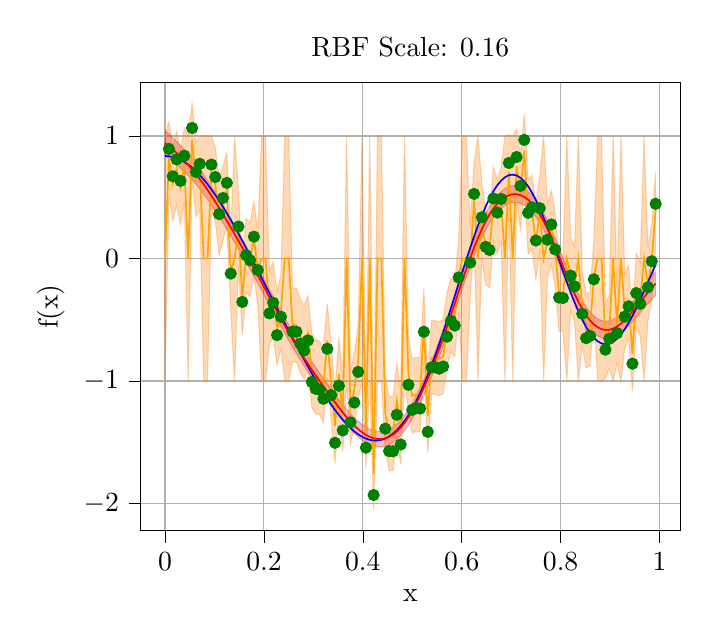
\begin{tikzpicture}

\definecolor{crimson2143940}{RGB}{214,39,40}
\definecolor{darkgray176}{RGB}{176,176,176}
\definecolor{darkorange25512714}{RGB}{255,127,14}
\definecolor{green}{RGB}{0,128,0}
\definecolor{lightgray204}{RGB}{204,204,204}
\definecolor{orange}{RGB}{255,165,0}

\begin{axis}[
legend cell align={left},
legend style={
  fill opacity=0,
  draw opacity=0,
  text opacity=0,
  at={(0.03,0.03)},
  anchor=south west,
  draw=lightgray204
},
tick align=outside,
tick pos=left,
title={RBF Scale: 0.16},
x grid style={darkgray176},
xlabel={x},
xmajorgrids,
xmin=-0.049609375, xmax=1.041796875,
xtick style={color=black},
y grid style={darkgray176},
ylabel={f(x)},
ymajorgrids,
ymin=-2.22237535963895, ymax=1.43635633210779,
ytick style={color=black}
]
\path [draw=darkorange25512714, fill=darkorange25512714, opacity=0.3]
(axis cs:0,1.00000000512856)
--(axis cs:0,-0.999999994871436)
--(axis cs:0.0078125,0.511444180197681)
--(axis cs:0.015625,0.308363006283013)
--(axis cs:0.0234375,0.434189823447664)
--(axis cs:0.03125,0.274352597986991)
--(axis cs:0.0390625,0.461344436540905)
--(axis cs:0.046875,-0.999999989077424)
--(axis cs:0.0546875,0.667027656963778)
--(axis cs:0.0625,0.340957621144296)
--(axis cs:0.0703125,0.401233676044626)
--(axis cs:0.078125,-0.999999995566704)
--(axis cs:0.0859375,-0.999999995605135)
--(axis cs:0.09375,0.395141799398463)
--(axis cs:0.1015625,0.302678668299754)
--(axis cs:0.109375,0.0280848565776906)
--(axis cs:0.1171875,0.147476675417313)
--(axis cs:0.125,0.25958144762537)
--(axis cs:0.1328125,-0.413248524080959)
--(axis cs:0.140625,-0.99999999921045)
--(axis cs:0.1484375,-0.0646185065363549)
--(axis cs:0.15625,-0.623902349234536)
--(axis cs:0.1640625,-0.277093368526466)
--(axis cs:0.171875,-0.314436311583211)
--(axis cs:0.1796875,-0.139372261644897)
--(axis cs:0.1875,-0.387273481986599)
--(axis cs:0.1953125,-1.00000000054103)
--(axis cs:0.203125,-1.00000000256758)
--(axis cs:0.2109375,-0.70851156347082)
--(axis cs:0.21875,-0.6297963814236)
--(axis cs:0.2265625,-0.869744103803077)
--(axis cs:0.234375,-0.733495949145235)
--(axis cs:0.2421875,-1.00000000272519)
--(axis cs:0.25,-1.0000000034232)
--(axis cs:0.2578125,-0.844140081857002)
--(axis cs:0.265625,-0.84507907624207)
--(axis cs:0.2734375,-0.932582615652796)
--(axis cs:0.28125,-0.983795732844705)
--(axis cs:0.2890625,-0.908684263615334)
--(axis cs:0.296875,-1.21782149670792)
--(axis cs:0.3046875,-1.2681825939875)
--(axis cs:0.3125,-1.27434691349112)
--(axis cs:0.3203125,-1.34252714098353)
--(axis cs:0.328125,-0.971260366884506)
--(axis cs:0.3359375,-1.3150147931128)
--(axis cs:0.34375,-1.66894889696598)
--(axis cs:0.3515625,-1.24562528675091)
--(axis cs:0.359375,-1.57707051721908)
--(axis cs:0.3671875,-1.00000001571806)
--(axis cs:0.375,-1.51750391519393)
--(axis cs:0.3828125,-1.37022418165687)
--(axis cs:0.390625,-1.14262470378849)
--(axis cs:0.3984375,-1.00000001416126)
--(axis cs:0.40625,-1.70517343381056)
--(axis cs:0.4140625,-1.00000001992376)
--(axis cs:0.421875,-2.05606937365046)
--(axis cs:0.4296875,-1.0000000110687)
--(axis cs:0.4375,-1.00000000796335)
--(axis cs:0.4453125,-1.5638229900427)
--(axis cs:0.453125,-1.73043253514964)
--(axis cs:0.4609375,-1.73195140042838)
--(axis cs:0.46875,-1.46110267653353)
--(axis cs:0.4765625,-1.68165671840965)
--(axis cs:0.484375,-1.00000001461787)
--(axis cs:0.4921875,-1.23852100507805)
--(axis cs:0.5,-1.42404877276762)
--(axis cs:0.5078125,-1.41107429362145)
--(axis cs:0.515625,-1.41485836495683)
--(axis cs:0.5234375,-0.845377599678533)
--(axis cs:0.53125,-1.58777488079117)
--(axis cs:0.5390625,-1.10939825931778)
--(axis cs:0.546875,-1.10909618323308)
--(axis cs:0.5546875,-1.11869345636539)
--(axis cs:0.5625,-1.10251200082666)
--(axis cs:0.5703125,-0.881281711785197)
--(axis cs:0.578125,-0.763676160554144)
--(axis cs:0.5859375,-0.79890126413386)
--(axis cs:0.59375,-0.442022145691459)
--(axis cs:0.6015625,-1.00000000088642)
--(axis cs:0.609375,-1.00000000019304)
--(axis cs:0.6171875,-0.332111208551257)
--(axis cs:0.625,0.177768478735485)
--(axis cs:0.6328125,-0.999999995045963)
--(axis cs:0.640625,0.00449922225988891)
--(axis cs:0.6484375,-0.214731023047178)
--(axis cs:0.65625,-0.238386536075759)
--(axis cs:0.6640625,0.144015789449179)
--(axis cs:0.671875,0.0391818108234269)
--(axis cs:0.6796875,0.140299957098084)
--(axis cs:0.6875,-0.999999992740988)
--(axis cs:0.6953125,0.407341345820018)
--(axis cs:0.703125,-0.99999999077952)
--(axis cs:0.7109375,0.451222627485389)
--(axis cs:0.71875,0.236940192270987)
--(axis cs:0.7265625,0.578480967228698)
--(axis cs:0.734375,0.0378251592761606)
--(axis cs:0.7421875,0.0774522233043436)
--(axis cs:0.75,-0.167777485860009)
--(axis cs:0.7578125,0.0719032468148578)
--(axis cs:0.765625,-0.999999996764793)
--(axis cs:0.7734375,-0.162096341052616)
--(axis cs:0.78125,-0.0489705884858324)
--(axis cs:0.7890625,-0.23444669552063)
--(axis cs:0.796875,-0.591444201919652)
--(axis cs:0.8046875,-0.594339511245762)
--(axis cs:0.8125,-1.00000000264708)
--(axis cs:0.8203125,-0.428285576895691)
--(axis cs:0.828125,-0.508479684423814)
--(axis cs:0.8359375,-1.00000000389306)
--(axis cs:0.84375,-0.711652698721024)
--(axis cs:0.8515625,-0.8925276525665)
--(axis cs:0.859375,-0.876142102815304)
--(axis cs:0.8671875,-0.455765387053987)
--(axis cs:0.875,-1.00000000097312)
--(axis cs:0.8828125,-1.0000000042671)
--(axis cs:0.890625,-0.977912222345866)
--(axis cs:0.8984375,-0.897266772070059)
--(axis cs:0.90625,-1.00000000725398)
--(axis cs:0.9140625,-0.855622120043601)
--(axis cs:0.921875,-1.00000000621546)
--(axis cs:0.9296875,-0.732645447518953)
--(axis cs:0.9375,-0.656345425748849)
--(axis cs:0.9453125,-1.08156286276021)
--(axis cs:0.953125,-0.558394688850909)
--(axis cs:0.9609375,-0.637255638481031)
--(axis cs:0.96875,-1.00000000346317)
--(axis cs:0.9765625,-0.514732295973921)
--(axis cs:0.984375,-0.321981568564207)
--(axis cs:0.9921875,0.104151395839067)
--(axis cs:0.9921875,0.707174084994594)
--(axis cs:0.9921875,0.707174084994594)
--(axis cs:0.984375,0.281041120591321)
--(axis cs:0.9765625,0.0882903931816071)
--(axis cs:0.96875,0.99999999653683)
--(axis cs:0.9609375,-0.0342329493255035)
--(axis cs:0.953125,0.0446280003046189)
--(axis cs:0.9453125,-0.478540173604684)
--(axis cs:0.9375,-0.0533227365933214)
--(axis cs:0.9296875,-0.129622758363426)
--(axis cs:0.921875,0.999999993784542)
--(axis cs:0.9140625,-0.252599430888074)
--(axis cs:0.90625,0.999999992746021)
--(axis cs:0.8984375,-0.294244082914531)
--(axis cs:0.890625,-0.374889533190338)
--(axis cs:0.8828125,0.999999995732897)
--(axis cs:0.875,0.999999999026882)
--(axis cs:0.8671875,0.14725730210154)
--(axis cs:0.859375,-0.273119413659776)
--(axis cs:0.8515625,-0.289504963410973)
--(axis cs:0.84375,-0.108630009565496)
--(axis cs:0.8359375,0.999999996106938)
--(axis cs:0.828125,0.0945430047317136)
--(axis cs:0.8203125,0.174737112259837)
--(axis cs:0.8125,0.999999997352921)
--(axis cs:0.8046875,0.00868317790976597)
--(axis cs:0.796875,0.0115784872358757)
--(axis cs:0.7890625,0.368575993634898)
--(axis cs:0.78125,0.554052100669695)
--(axis cs:0.7734375,0.440926348102911)
--(axis cs:0.765625,1.00000000323521)
--(axis cs:0.7578125,0.674925935970385)
--(axis cs:0.75,0.435245203295519)
--(axis cs:0.7421875,0.680474912459871)
--(axis cs:0.734375,0.640847848431688)
--(axis cs:0.7265625,1.18150365638423)
--(axis cs:0.71875,0.839962881426515)
--(axis cs:0.7109375,1.05424531664092)
--(axis cs:0.703125,1.00000000922048)
--(axis cs:0.6953125,1.01036403497555)
--(axis cs:0.6875,1.00000000725901)
--(axis cs:0.6796875,0.743322646253612)
--(axis cs:0.671875,0.642204499978955)
--(axis cs:0.6640625,0.747038478604707)
--(axis cs:0.65625,0.364636153079768)
--(axis cs:0.6484375,0.38829166610835)
--(axis cs:0.640625,0.607521911415417)
--(axis cs:0.6328125,1.00000000495404)
--(axis cs:0.625,0.780791167891012)
--(axis cs:0.6171875,0.270911480604271)
--(axis cs:0.609375,0.999999999806959)
--(axis cs:0.6015625,0.999999999113582)
--(axis cs:0.59375,0.161000543464069)
--(axis cs:0.5859375,-0.195878574978332)
--(axis cs:0.578125,-0.160653471398617)
--(axis cs:0.5703125,-0.27825902262967)
--(axis cs:0.5625,-0.499489311671135)
--(axis cs:0.5546875,-0.515670767209863)
--(axis cs:0.546875,-0.506073494077551)
--(axis cs:0.5390625,-0.506375570162253)
--(axis cs:0.53125,-0.984752191635645)
--(axis cs:0.5234375,-0.242354910523005)
--(axis cs:0.515625,-0.811835675801306)
--(axis cs:0.5078125,-0.808051604465918)
--(axis cs:0.5,-0.82102608361209)
--(axis cs:0.4921875,-0.635498315922527)
--(axis cs:0.484375,0.999999985382131)
--(axis cs:0.4765625,-1.07863402925412)
--(axis cs:0.46875,-0.858079987378002)
--(axis cs:0.4609375,-1.12892871127285)
--(axis cs:0.453125,-1.12740984599411)
--(axis cs:0.4453125,-0.960800300887174)
--(axis cs:0.4375,0.999999992036655)
--(axis cs:0.4296875,0.999999988931298)
--(axis cs:0.421875,-1.45304668449494)
--(axis cs:0.4140625,0.999999980076237)
--(axis cs:0.40625,-1.10215074465503)
--(axis cs:0.3984375,0.999999985838741)
--(axis cs:0.390625,-0.539602014632959)
--(axis cs:0.3828125,-0.767201492501342)
--(axis cs:0.375,-0.914481226038405)
--(axis cs:0.3671875,0.999999984281942)
--(axis cs:0.359375,-0.97404782806355)
--(axis cs:0.3515625,-0.642602597595385)
--(axis cs:0.34375,-1.06592620781045)
--(axis cs:0.3359375,-0.711992103957269)
--(axis cs:0.328125,-0.368237677728979)
--(axis cs:0.3203125,-0.739504451828007)
--(axis cs:0.3125,-0.671324224335589)
--(axis cs:0.3046875,-0.665159904831976)
--(axis cs:0.296875,-0.614798807552393)
--(axis cs:0.2890625,-0.305661574459807)
--(axis cs:0.28125,-0.380773043689177)
--(axis cs:0.2734375,-0.329559926497268)
--(axis cs:0.265625,-0.242056387086542)
--(axis cs:0.2578125,-0.241117392701474)
--(axis cs:0.25,0.999999996576804)
--(axis cs:0.2421875,0.999999997274807)
--(axis cs:0.234375,-0.130473259989707)
--(axis cs:0.2265625,-0.26672141464755)
--(axis cs:0.21875,-0.0267736922680725)
--(axis cs:0.2109375,-0.105488874315293)
--(axis cs:0.203125,0.999999997432422)
--(axis cs:0.1953125,0.999999999458966)
--(axis cs:0.1875,0.215749207168929)
--(axis cs:0.1796875,0.463650427510631)
--(axis cs:0.171875,0.288586377572317)
--(axis cs:0.1640625,0.325929320629062)
--(axis cs:0.15625,-0.0208796600790086)
--(axis cs:0.1484375,0.538404182619173)
--(axis cs:0.140625,1.00000000078955)
--(axis cs:0.1328125,0.189774165074569)
--(axis cs:0.125,0.862604136780898)
--(axis cs:0.1171875,0.75049936457284)
--(axis cs:0.109375,0.631107545733218)
--(axis cs:0.1015625,0.905701357455281)
--(axis cs:0.09375,0.99816448855399)
--(axis cs:0.0859375,1.00000000439487)
--(axis cs:0.078125,1.0000000044333)
--(axis cs:0.0703125,1.00425636520015)
--(axis cs:0.0625,0.943980310299824)
--(axis cs:0.0546875,1.27005034611931)
--(axis cs:0.046875,1.00000001092258)
--(axis cs:0.0390625,1.06436712569643)
--(axis cs:0.03125,0.877375287142518)
--(axis cs:0.0234375,1.03721251260319)
--(axis cs:0.015625,0.91138569543854)
--(axis cs:0.0078125,1.11446686935321)
--(axis cs:0,1.00000000512856)
--cycle;

\addplot [draw=green, fill=green, mark=*, only marks]
table{%
x  y
0.0078125 0.894251048564911
0.015625 0.670861780643463
0.0234375 0.809271275997162
0.03125 0.633450329303741
0.0390625 0.839141368865967
0.0546875 1.06539285182953
0.0625 0.706715881824493
0.0703125 0.77301949262619
0.09375 0.766318440437317
0.1015625 0.664609014987946
0.109375 0.362555831670761
0.1171875 0.493886828422546
0.125 0.617202043533325
0.1328125 -0.122910894453526
0.1484375 0.260582119226456
0.15625 -0.35463011264801
0.1640625 0.0268597733229399
0.171875 -0.0142174642533064
0.1796875 0.178352996706963
0.1875 -0.0943383499979973
0.2109375 -0.44770023226738
0.21875 -0.361113548278809
0.2265625 -0.625056028366089
0.234375 -0.475183069705963
0.2578125 -0.596891582012177
0.265625 -0.597924530506134
0.2734375 -0.694178402423859
0.28125 -0.750512838363647
0.2890625 -0.667890191078186
0.296875 -1.00794112682343
0.3046875 -1.06333839893341
0.3125 -1.07011914253235
0.3203125 -1.14511740207672
0.328125 -0.736723899841309
0.3359375 -1.11485373973846
0.34375 -1.50418126583099
0.3515625 -1.03852534294128
0.359375 -1.40311503410339
0.375 -1.33759188652039
0.3828125 -1.17558407783508
0.390625 -0.925224721431732
0.40625 -1.54402828216553
0.421875 -1.9300137758255
0.4453125 -1.38854277133942
0.453125 -1.57181334495544
0.4609375 -1.5734840631485
0.46875 -1.27555048465729
0.4765625 -1.51815986633301
0.4921875 -1.03071057796478
0.5 -1.23479115962982
0.5078125 -1.22051918506622
0.515625 -1.22468173503876
0.5234375 -0.598252892494202
0.53125 -1.41488993167877
0.5390625 -0.888675630092621
0.546875 -0.888343334197998
0.5546875 -0.898900330066681
0.5625 -0.881100714206696
0.5703125 -0.637747406959534
0.578125 -0.508381307125092
0.5859375 -0.547128915786743
0.59375 -0.154561877250671
0.6171875 -0.0336598493158817
0.625 0.527207791805267
0.640625 0.33661162853241
0.6484375 0.0954583510756493
0.65625 0.06943728774786
0.6640625 0.49007984995842
0.671875 0.37476247549057
0.6796875 0.485992431640625
0.6953125 0.779737949371338
0.7109375 0.828007340431213
0.71875 0.592296659946442
0.7265625 0.967991530895233
0.734375 0.373270153999329
0.7421875 0.416859924793243
0.75 0.147107243537903
0.7578125 0.410756051540375
0.7734375 0.15335650742054
0.78125 0.27779483795166
0.7890625 0.0737711116671562
0.796875 -0.318926155567169
0.8046875 -0.32211098074913
0.8203125 -0.139451652765274
0.828125 -0.227665171027184
0.84375 -0.451155483722687
0.8515625 -0.650117933750153
0.859375 -0.632093846797943
0.8671875 -0.169679448008537
0.890625 -0.744040966033936
0.8984375 -0.655330955982208
0.9140625 -0.609521865844727
0.9296875 -0.474247515201569
0.9375 -0.390317499637604
0.9453125 -0.858056664466858
0.953125 -0.28257167339325
0.9609375 -0.369318723678589
0.9765625 -0.234543040394783
0.984375 -0.0225172471255064
0.9921875 0.446229010820389
};
\addlegendentry{context points}
\path [draw=crimson2143940, fill=crimson2143940, opacity=0.3]
(axis cs:0,1.04651010036469)
--(axis cs:0,0.839118361473083)
--(axis cs:0.0078125,0.816638231277466)
--(axis cs:0.015625,0.792373657226562)
--(axis cs:0.0234375,0.766547203063965)
--(axis cs:0.03125,0.738702118396759)
--(axis cs:0.0390625,0.708943247795105)
--(axis cs:0.046875,0.676824986934662)
--(axis cs:0.0546875,0.642575621604919)
--(axis cs:0.0625,0.606275737285614)
--(axis cs:0.0703125,0.567110002040863)
--(axis cs:0.078125,0.526220560073853)
--(axis cs:0.0859375,0.482536733150482)
--(axis cs:0.09375,0.436638832092285)
--(axis cs:0.1015625,0.389019250869751)
--(axis cs:0.109375,0.339724957942963)
--(axis cs:0.1171875,0.288868635892868)
--(axis cs:0.125,0.23679593205452)
--(axis cs:0.1328125,0.184134647250175)
--(axis cs:0.140625,0.13066740334034)
--(axis cs:0.1484375,0.076462022960186)
--(axis cs:0.15625,0.0219074711203575)
--(axis cs:0.1640625,-0.0331324636936188)
--(axis cs:0.171875,-0.0887844264507294)
--(axis cs:0.1796875,-0.145233854651451)
--(axis cs:0.1875,-0.202162683010101)
--(axis cs:0.1953125,-0.260114341974258)
--(axis cs:0.203125,-0.31843638420105)
--(axis cs:0.2109375,-0.377377152442932)
--(axis cs:0.21875,-0.436529874801636)
--(axis cs:0.2265625,-0.495138615369797)
--(axis cs:0.234375,-0.553621590137482)
--(axis cs:0.2421875,-0.611133217811584)
--(axis cs:0.25,-0.667466998100281)
--(axis cs:0.2578125,-0.722219944000244)
--(axis cs:0.265625,-0.775302231311798)
--(axis cs:0.2734375,-0.826837837696075)
--(axis cs:0.28125,-0.876543402671814)
--(axis cs:0.2890625,-0.924874901771545)
--(axis cs:0.296875,-0.971706032752991)
--(axis cs:0.3046875,-1.01770079135895)
--(axis cs:0.3125,-1.06293869018555)
--(axis cs:0.3203125,-1.10742509365082)
--(axis cs:0.328125,-1.15167152881622)
--(axis cs:0.3359375,-1.1951357126236)
--(axis cs:0.34375,-1.2381477355957)
--(axis cs:0.3515625,-1.28009271621704)
--(axis cs:0.359375,-1.32061052322388)
--(axis cs:0.3671875,-1.35924732685089)
--(axis cs:0.375,-1.39519739151001)
--(axis cs:0.3828125,-1.42803454399109)
--(axis cs:0.390625,-1.45751857757568)
--(axis cs:0.3984375,-1.48278284072876)
--(axis cs:0.40625,-1.50370538234711)
--(axis cs:0.4140625,-1.51980137825012)
--(axis cs:0.421875,-1.53084218502045)
--(axis cs:0.4296875,-1.53656697273254)
--(axis cs:0.4375,-1.53660869598389)
--(axis cs:0.4453125,-1.53107726573944)
--(axis cs:0.453125,-1.51912593841553)
--(axis cs:0.4609375,-1.50079441070557)
--(axis cs:0.46875,-1.47582387924194)
--(axis cs:0.4765625,-1.44373202323914)
--(axis cs:0.484375,-1.40478205680847)
--(axis cs:0.4921875,-1.3589608669281)
--(axis cs:0.5,-1.30679249763489)
--(axis cs:0.5078125,-1.24878621101379)
--(axis cs:0.515625,-1.18545949459076)
--(axis cs:0.5234375,-1.11725103855133)
--(axis cs:0.53125,-1.04450523853302)
--(axis cs:0.5390625,-0.967800080776215)
--(axis cs:0.546875,-0.887167096138)
--(axis cs:0.5546875,-0.802599132061005)
--(axis cs:0.5625,-0.714339256286621)
--(axis cs:0.5703125,-0.623007297515869)
--(axis cs:0.578125,-0.529096364974976)
--(axis cs:0.5859375,-0.433818995952606)
--(axis cs:0.59375,-0.338235467672348)
--(axis cs:0.6015625,-0.243863701820374)
--(axis cs:0.609375,-0.15178382396698)
--(axis cs:0.6171875,-0.0630647018551826)
--(axis cs:0.625,0.0205037295818329)
--(axis cs:0.6328125,0.0983819216489792)
--(axis cs:0.640625,0.169680401682854)
--(axis cs:0.6484375,0.233405843377113)
--(axis cs:0.65625,0.289621651172638)
--(axis cs:0.6640625,0.337801277637482)
--(axis cs:0.671875,0.377555847167969)
--(axis cs:0.6796875,0.409142136573792)
--(axis cs:0.6875,0.432689100503922)
--(axis cs:0.6953125,0.44836151599884)
--(axis cs:0.703125,0.45625177025795)
--(axis cs:0.7109375,0.456461608409882)
--(axis cs:0.71875,0.449167370796204)
--(axis cs:0.7265625,0.433993458747864)
--(axis cs:0.734375,0.411077618598938)
--(axis cs:0.7421875,0.379957109689713)
--(axis cs:0.75,0.340478777885437)
--(axis cs:0.7578125,0.292981445789337)
--(axis cs:0.765625,0.237180322408676)
--(axis cs:0.7734375,0.174164950847626)
--(axis cs:0.78125,0.104836493730545)
--(axis cs:0.7890625,0.0302081182599068)
--(axis cs:0.796875,-0.047587014734745)
--(axis cs:0.8046875,-0.126953631639481)
--(axis cs:0.8125,-0.206130921840668)
--(axis cs:0.8203125,-0.28199166059494)
--(axis cs:0.828125,-0.35383015871048)
--(axis cs:0.8359375,-0.419822573661804)
--(axis cs:0.84375,-0.478821158409119)
--(axis cs:0.8515625,-0.529708325862885)
--(axis cs:0.859375,-0.57241827249527)
--(axis cs:0.8671875,-0.606015920639038)
--(axis cs:0.875,-0.630993843078613)
--(axis cs:0.8828125,-0.646959543228149)
--(axis cs:0.890625,-0.654519557952881)
--(axis cs:0.8984375,-0.653807997703552)
--(axis cs:0.90625,-0.645469188690186)
--(axis cs:0.9140625,-0.630167901515961)
--(axis cs:0.921875,-0.60867178440094)
--(axis cs:0.9296875,-0.581784248352051)
--(axis cs:0.9375,-0.550618052482605)
--(axis cs:0.9453125,-0.516427516937256)
--(axis cs:0.953125,-0.479791134595871)
--(axis cs:0.9609375,-0.442436277866364)
--(axis cs:0.96875,-0.405153155326843)
--(axis cs:0.9765625,-0.368854165077209)
--(axis cs:0.984375,-0.334431141614914)
--(axis cs:0.9921875,-0.302232474088669)
--(axis cs:0.9921875,-0.106797493994236)
--(axis cs:0.9921875,-0.106797493994236)
--(axis cs:0.984375,-0.145401507616043)
--(axis cs:0.9765625,-0.185808286070824)
--(axis cs:0.96875,-0.227708473801613)
--(axis cs:0.9609375,-0.270123422145844)
--(axis cs:0.953125,-0.312235623598099)
--(axis cs:0.9453125,-0.353226155042648)
--(axis cs:0.9375,-0.391382813453674)
--(axis cs:0.9296875,-0.426187515258789)
--(axis cs:0.921875,-0.456325650215149)
--(axis cs:0.9140625,-0.480768740177155)
--(axis cs:0.90625,-0.49871090054512)
--(axis cs:0.8984375,-0.509413838386536)
--(axis cs:0.890625,-0.512228488922119)
--(axis cs:0.8828125,-0.506512880325317)
--(axis cs:0.875,-0.492155790328979)
--(axis cs:0.8671875,-0.468579322099686)
--(axis cs:0.859375,-0.436166703701019)
--(axis cs:0.8515625,-0.394453376531601)
--(axis cs:0.84375,-0.344380974769592)
--(axis cs:0.8359375,-0.28603732585907)
--(axis cs:0.828125,-0.220546647906303)
--(axis cs:0.8203125,-0.149057686328888)
--(axis cs:0.8125,-0.0734067633748055)
--(axis cs:0.8046875,0.00566843152046204)
--(axis cs:0.796875,0.0850573554635048)
--(axis cs:0.7890625,0.162972688674927)
--(axis cs:0.78125,0.237804144620895)
--(axis cs:0.7734375,0.307404577732086)
--(axis cs:0.765625,0.370750576257706)
--(axis cs:0.7578125,0.426939427852631)
--(axis cs:0.75,0.474838137626648)
--(axis cs:0.7421875,0.514741778373718)
--(axis cs:0.734375,0.546290040016174)
--(axis cs:0.7265625,0.569628834724426)
--(axis cs:0.71875,0.585188984870911)
--(axis cs:0.7109375,0.59285694360733)
--(axis cs:0.703125,0.592984795570374)
--(axis cs:0.6953125,0.585394501686096)
--(axis cs:0.6875,0.569980502128601)
--(axis cs:0.6796875,0.546630024909973)
--(axis cs:0.671875,0.515194654464722)
--(axis cs:0.6640625,0.475519597530365)
--(axis cs:0.65625,0.427373349666595)
--(axis cs:0.6484375,0.371113300323486)
--(axis cs:0.640625,0.307292878627777)
--(axis cs:0.6328125,0.235815361142159)
--(axis cs:0.625,0.15769961476326)
--(axis cs:0.6171875,0.0738200023770332)
--(axis cs:0.609375,-0.015290379524231)
--(axis cs:0.6015625,-0.107823260128498)
--(axis cs:0.59375,-0.202718645334244)
--(axis cs:0.5859375,-0.298882067203522)
--(axis cs:0.578125,-0.394792079925537)
--(axis cs:0.5703125,-0.489373415708542)
--(axis cs:0.5625,-0.581417798995972)
--(axis cs:0.5546875,-0.670394480228424)
--(axis cs:0.546875,-0.755694985389709)
--(axis cs:0.5390625,-0.8370321393013)
--(axis cs:0.53125,-0.914432227611542)
--(axis cs:0.5234375,-0.987806439399719)
--(axis cs:0.515625,-1.05660307407379)
--(axis cs:0.5078125,-1.12044358253479)
--(axis cs:0.5,-1.17889070510864)
--(axis cs:0.4921875,-1.23142123222351)
--(axis cs:0.484375,-1.27751326560974)
--(axis cs:0.4765625,-1.31667232513428)
--(axis cs:0.46875,-1.34889221191406)
--(axis cs:0.4609375,-1.37390661239624)
--(axis cs:0.453125,-1.39221858978271)
--(axis cs:0.4453125,-1.40410006046295)
--(axis cs:0.4375,-1.40950727462769)
--(axis cs:0.4296875,-1.40930247306824)
--(axis cs:0.421875,-1.40338575839996)
--(axis cs:0.4140625,-1.39213490486145)
--(axis cs:0.40625,-1.37582314014435)
--(axis cs:0.3984375,-1.35469818115234)
--(axis cs:0.390625,-1.32924032211304)
--(axis cs:0.3828125,-1.29956912994385)
--(axis cs:0.375,-1.26657772064209)
--(axis cs:0.3671875,-1.23051488399506)
--(axis cs:0.359375,-1.19179725646973)
--(axis cs:0.3515625,-1.15124034881592)
--(axis cs:0.34375,-1.109299659729)
--(axis cs:0.3359375,-1.06633508205414)
--(axis cs:0.328125,-1.02296721935272)
--(axis cs:0.3203125,-0.978867650032043)
--(axis cs:0.3125,-0.934564411640167)
--(axis cs:0.3046875,-0.889539837837219)
--(axis cs:0.296875,-0.843781113624573)
--(axis cs:0.2890625,-0.797202467918396)
--(axis cs:0.28125,-0.749120593070984)
--(axis cs:0.2734375,-0.699665248394012)
--(axis cs:0.265625,-0.648334920406342)
--(axis cs:0.2578125,-0.59541916847229)
--(axis cs:0.25,-0.540763974189758)
--(axis cs:0.2421875,-0.484452128410339)
--(axis cs:0.234375,-0.426870286464691)
--(axis cs:0.2265625,-0.368218690156937)
--(axis cs:0.21875,-0.309323310852051)
--(axis cs:0.2109375,-0.24975810945034)
--(axis cs:0.203125,-0.190291181206703)
--(axis cs:0.1953125,-0.131305307149887)
--(axis cs:0.1875,-0.072557270526886)
--(axis cs:0.1796875,-0.0146834999322891)
--(axis cs:0.171875,0.0428414046764374)
--(axis cs:0.1640625,0.0997191965579987)
--(axis cs:0.15625,0.15612468123436)
--(axis cs:0.1484375,0.212210655212402)
--(axis cs:0.140625,0.268111765384674)
--(axis cs:0.1328125,0.323427736759186)
--(axis cs:0.125,0.378109186887741)
--(axis cs:0.1171875,0.432388335466385)
--(axis cs:0.109375,0.485630810260773)
--(axis cs:0.1015625,0.537520885467529)
--(axis cs:0.09375,0.587958574295044)
--(axis cs:0.0859375,0.636891186237335)
--(axis cs:0.078125,0.683844566345215)
--(axis cs:0.0703125,0.728249371051788)
--(axis cs:0.0625,0.771234571933746)
--(axis cs:0.0546875,0.811639666557312)
--(axis cs:0.046875,0.850292026996613)
--(axis cs:0.0390625,0.887146353721619)
--(axis cs:0.03125,0.922004640102386)
--(axis cs:0.0234375,0.955294370651245)
--(axis cs:0.015625,0.98694634437561)
--(axis cs:0.0078125,1.01739120483398)
--(axis cs:0,1.04651010036469)
--cycle;

\addplot [semithick, orange]
table {%
0 5.12856361912367e-09
0.0078125 0.812955524775445
0.015625 0.609874350860776
0.0234375 0.735701168025428
0.03125 0.575863942564754
0.0390625 0.762855781118668
0.046875 1.09225757433046e-08
0.0546875 0.968539001541542
0.0625 0.64246896572206
0.0703125 0.70274502062239
0.078125 4.43329608166473e-09
0.0859375 4.39486522672047e-09
0.09375 0.696653143976226
0.1015625 0.604190012877518
0.109375 0.329596201155454
0.1171875 0.448988019995077
0.125 0.561092792203134
0.1328125 -0.111737179503195
0.140625 7.89549652914482e-10
0.1484375 0.236892838041409
0.15625 -0.322391004656772
0.1640625 0.0244179760512977
0.171875 -0.0129249670054473
0.1796875 0.162139082932867
0.1875 -0.0857621374088346
0.1953125 -5.41034007071999e-10
0.203125 -2.56757774716432e-09
0.2109375 -0.407000218893056
0.21875 -0.328285036845836
0.2265625 -0.568232759225313
0.234375 -0.431984604567471
0.2421875 -2.72519277080852e-09
0.25 -3.42319587169755e-09
0.2578125 -0.542628737279238
0.265625 -0.543567731664306
0.2734375 -0.631071271075032
0.28125 -0.682284388266941
0.2890625 -0.607172919037571
0.296875 -0.916310152130157
0.3046875 -0.96667124940974
0.3125 -0.972835568913353
0.3203125 -1.04101579640577
0.328125 -0.669749022306742
0.3359375 -1.01350344853503
0.34375 -1.36743755238821
0.3515625 -0.944113942173149
0.359375 -1.27555917264131
0.3671875 -1.5718057423272e-08
0.375 -1.21599257061617
0.3828125 -1.06871283707911
0.390625 -0.841113359210723
0.3984375 -1.41612589705655e-08
0.40625 -1.40366208923279
0.4140625 -1.99237625958153e-08
0.421875 -1.7545580290727
0.4296875 -1.10687020924226e-08
0.4375 -7.9633453098464e-09
0.4453125 -1.26231164546494
0.453125 -1.42892119057187
0.4609375 -1.43044005585061
0.46875 -1.15959133195577
0.4765625 -1.38014537383188
0.484375 -1.4617868541618e-08
0.4921875 -0.937009660500291
0.5 -1.12253742818985
0.5078125 -1.10956294904368
0.515625 -1.11334702037907
0.5234375 -0.543866255100769
0.53125 -1.28626353621341
0.5390625 -0.807886914740017
0.546875 -0.807584838655315
0.5546875 -0.817182111787626
0.5625 -0.801000656248899
0.5703125 -0.579770367207434
0.578125 -0.46216481597638
0.5859375 -0.497389919556096
0.59375 -0.140510801113695
0.6015625 -8.86418196374064e-10
0.609375 -1.93040530005784e-10
0.6171875 -0.030599863973493
0.625 0.479279823313249
0.6328125 4.95403699203695e-09
0.640625 0.306010566837653
0.6484375 0.0867803215305861
0.65625 0.0631248085020044
0.6640625 0.445527134026943
0.671875 0.340693155401191
0.6796875 0.441811301675848
0.6875 7.2590115014226e-09
0.6953125 0.708852690397782
0.703125 9.22048005444977e-09
0.7109375 0.752733972063153
0.71875 0.538451536848751
0.7265625 0.879992311806462
0.734375 0.339336503853924
0.7421875 0.378963567882107
0.75 0.133733858717755
0.7578125 0.373414591392622
0.765625 3.23520675252446e-09
0.7734375 0.139415003525147
0.78125 0.252540756091931
0.7890625 0.0670646490571339
0.796875 -0.289932857341888
0.8046875 -0.292828166667998
0.8125 -2.64707911621482e-09
0.8203125 -0.126774232317927
0.828125 -0.20696833984605
0.8359375 -3.89306206908686e-09
0.84375 -0.41014135414326
0.8515625 -0.591016307988737
0.859375 -0.57463075823754
0.8671875 -0.154254042476223
0.875 -9.73118001403032e-10
0.8828125 -4.26710296576655e-09
0.890625 -0.676400877768102
0.8984375 -0.595755427492295
0.90625 -7.25397860234023e-09
0.9140625 -0.554110775465838
0.921875 -6.21545816194111e-09
0.9296875 -0.431134102941189
0.9375 -0.354834081171085
0.9453125 -0.780051518182448
0.953125 -0.256883344273145
0.9609375 -0.335744293903267
0.96875 -3.46317000593004e-09
0.9765625 -0.213220951396157
0.984375 -0.0204702239864428
0.9921875 0.40566274041683
};
\addlegendentry{gp prediction}
\addplot [semithick, blue]
table {%
0 0.836456000804901
0.0078125 0.83406388759613
0.015625 0.828014194965363
0.0234375 0.818231046199799
0.03125 0.804663836956024
0.0390625 0.787291824817657
0.046875 0.766124784946442
0.0546875 0.74120432138443
0.0625 0.712604701519012
0.0703125 0.680431604385376
0.078125 0.644821166992188
0.0859375 0.605936765670776
0.09375 0.563966751098633
0.1015625 0.51911997795105
0.109375 0.471622109413147
0.1171875 0.42171037197113
0.125 0.369629055261612
0.1328125 0.315624684095383
0.140625 0.259940952062607
0.1484375 0.202815338969231
0.15625 0.144474670290947
0.1640625 0.0851323530077934
0.171875 0.0249861162155867
0.1796875 -0.0357830934226513
0.1875 -0.0970124304294586
0.1953125 -0.158555388450623
0.203125 -0.220282062888145
0.2109375 -0.282075941562653
0.21875 -0.343832105398178
0.2265625 -0.405454009771347
0.234375 -0.466849327087402
0.2421875 -0.527927339076996
0.25 -0.588594615459442
0.2578125 -0.64875203371048
0.265625 -0.708291411399841
0.2734375 -0.767093002796173
0.28125 -0.825023055076599
0.2890625 -0.881932735443115
0.296875 -0.937657415866852
0.3046875 -0.992015600204468
0.3125 -1.04480993747711
0.3203125 -1.0958286523819
0.328125 -1.14484584331512
0.3359375 -1.19162440299988
0.34375 -1.23591697216034
0.3515625 -1.27746939659119
0.359375 -1.31602203845978
0.3671875 -1.3513126373291
0.375 -1.38307845592499
0.3828125 -1.41105794906616
0.390625 -1.43499338626862
0.3984375 -1.45463180541992
0.40625 -1.4697277545929
0.4140625 -1.48004353046417
0.421875 -1.48535263538361
0.4296875 -1.48543989658356
0.4375 -1.48010456562042
0.4453125 -1.46916222572327
0.453125 -1.45244812965393
0.4609375 -1.42981910705566
0.46875 -1.40115904808044
0.4765625 -1.36638176441193
0.484375 -1.32543659210205
0.4921875 -1.27831315994263
0.5 -1.22504699230194
0.5078125 -1.16572570800781
0.515625 -1.10049414634705
0.5234375 -1.02956140041351
0.53125 -0.95320463180542
0.5390625 -0.87177437543869
0.546875 -0.785699069499969
0.5546875 -0.695487141609192
0.5625 -0.601728081703186
0.5703125 -0.505093634128571
0.578125 -0.406333774328232
0.5859375 -0.306274503469467
0.59375 -0.205810412764549
0.6015625 -0.105897657573223
0.609375 -0.00754218269139528
0.6171875 0.0882117226719856
0.625 0.180296689271927
0.6328125 0.267638951539993
0.640625 0.349175125360489
0.6484375 0.423873007297516
0.65625 0.490750461816788
0.6640625 0.548896610736847
0.671875 0.597491860389709
0.6796875 0.635828256607056
0.6875 0.663327395915985
0.6953125 0.679557800292969
0.703125 0.684250354766846
0.7109375 0.677309155464172
0.71875 0.658821284770966
0.7265625 0.629061758518219
0.734375 0.588495254516602
0.7421875 0.53777289390564
0.75 0.477725833654404
0.7578125 0.409354120492935
0.765625 0.33381113409996
0.7734375 0.252384781837463
0.78125 0.166474655270576
0.7890625 0.0775668099522591
0.796875 -0.0127944126725197
0.8046875 -0.103037312626839
0.8125 -0.191592067480087
0.8203125 -0.276923507452011
0.828125 -0.357561975717545
0.8359375 -0.432132065296173
0.84375 -0.499381512403488
0.8515625 -0.558205604553223
0.859375 -0.607669293880463
0.8671875 -0.647024929523468
0.875 -0.675725936889648
0.8828125 -0.693435430526733
0.890625 -0.700031220912933
0.8984375 -0.69560432434082
0.90625 -0.680453240871429
0.9140625 -0.655074536800385
0.921875 -0.620147228240967
0.9296875 -0.576515436172485
0.9375 -0.525165498256683
0.9453125 -0.467202246189117
0.953125 -0.403820902109146
0.9609375 -0.336280345916748
0.96875 -0.265872418880463
0.9765625 -0.193894401192665
0.984375 -0.121619656682014
0.9921875 -0.0502712689340115
};
\addlegendentry{target}
\addplot [semithick, red]
table {%
0 0.942814230918884
0.0078125 0.917014718055725
0.015625 0.889660000801086
0.0234375 0.860920786857605
0.03125 0.830353379249573
0.0390625 0.798044800758362
0.046875 0.763558506965637
0.0546875 0.727107644081116
0.0625 0.68875515460968
0.0703125 0.647679686546326
0.078125 0.605032563209534
0.0859375 0.559713959693909
0.09375 0.512298703193665
0.1015625 0.46327006816864
0.109375 0.412677884101868
0.1171875 0.360628485679626
0.125 0.30745255947113
0.1328125 0.253781199455261
0.140625 0.199389576911926
0.1484375 0.144336342811584
0.15625 0.0890160799026489
0.1640625 0.0332933664321899
0.171875 -0.022971510887146
0.1796875 -0.0799586772918701
0.1875 -0.137359976768494
0.1953125 -0.195709824562073
0.203125 -0.254363775253296
0.2109375 -0.313567638397217
0.21875 -0.372926592826843
0.2265625 -0.431678652763367
0.234375 -0.490245938301086
0.2421875 -0.547792673110962
0.25 -0.60411548614502
0.2578125 -0.658819556236267
0.265625 -0.71181857585907
0.2734375 -0.763251543045044
0.28125 -0.812831997871399
0.2890625 -0.861038684844971
0.296875 -0.907743573188782
0.3046875 -0.953620314598083
0.3125 -0.998751580715179
0.3203125 -1.04314637184143
0.328125 -1.08731937408447
0.3359375 -1.13073539733887
0.34375 -1.17372369766235
0.3515625 -1.21566653251648
0.359375 -1.2562038898468
0.3671875 -1.29488110542297
0.375 -1.33088755607605
0.3828125 -1.36380183696747
0.390625 -1.39337944984436
0.3984375 -1.41874051094055
0.40625 -1.43976426124573
0.4140625 -1.45596814155579
0.421875 -1.46711397171021
0.4296875 -1.47293472290039
0.4375 -1.47305798530579
0.4453125 -1.4675886631012
0.453125 -1.45567226409912
0.4609375 -1.4373505115509
0.46875 -1.412358045578
0.4765625 -1.38020217418671
0.484375 -1.34114766120911
0.4921875 -1.29519104957581
0.5 -1.24284160137177
0.5078125 -1.18461489677429
0.515625 -1.12103128433228
0.5234375 -1.05252873897552
0.53125 -0.979468703269958
0.5390625 -0.902416110038757
0.546875 -0.821431040763855
0.5546875 -0.736496806144714
0.5625 -0.647878527641296
0.5703125 -0.556190371513367
0.578125 -0.461944222450256
0.5859375 -0.366350531578064
0.59375 -0.270477056503296
0.6015625 -0.175843477249146
0.609375 -0.0835371017456055
0.6171875 0.00537765026092529
0.625 0.0891016721725464
0.6328125 0.167098641395569
0.640625 0.238486647605896
0.6484375 0.302259564399719
0.65625 0.358497500419617
0.6640625 0.406660437583923
0.671875 0.446375250816345
0.6796875 0.477886080741882
0.6875 0.5013347864151
0.6953125 0.516878008842468
0.703125 0.524618268013
0.7109375 0.524659276008606
0.71875 0.517178177833557
0.7265625 0.501811146736145
0.734375 0.478683829307556
0.7421875 0.447349429130554
0.75 0.407658457756042
0.7578125 0.359960436820984
0.765625 0.303965449333191
0.7734375 0.240784764289856
0.78125 0.17132031917572
0.7890625 0.0965903997421265
0.796875 0.0187351703643799
0.8046875 -0.0606426000595093
0.8125 -0.139768838882446
0.8203125 -0.215524673461914
0.828125 -0.287188410758972
0.8359375 -0.352929949760437
0.84375 -0.411601066589355
0.8515625 -0.462080836296082
0.859375 -0.504292488098145
0.8671875 -0.537297606468201
0.875 -0.561574816703796
0.8828125 -0.576736211776733
0.890625 -0.5833740234375
0.8984375 -0.581610918045044
0.90625 -0.572090029716492
0.9140625 -0.555468320846558
0.921875 -0.532498717308044
0.9296875 -0.50398588180542
0.9375 -0.47100043296814
0.9453125 -0.434826850891113
0.953125 -0.396013379096985
0.9609375 -0.356279850006104
0.96875 -0.316430807113647
0.9765625 -0.277331233024597
0.984375 -0.239916324615479
0.9921875 -0.204514980316162
};
\addlegendentry{prediction}
\end{axis}

\end{tikzpicture}

		% This file was created with matplot2tikz v0.4.0.
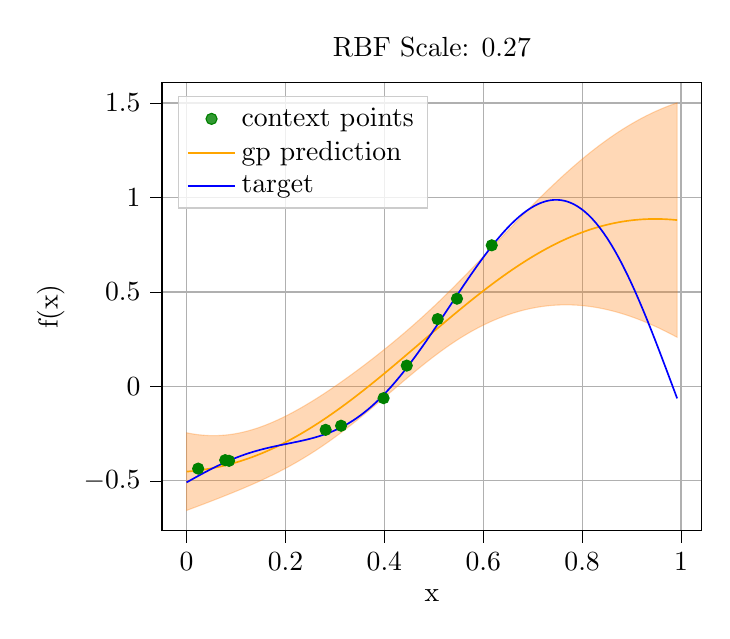
\begin{tikzpicture}

\definecolor{darkgray176}{RGB}{176,176,176}
\definecolor{darkorange25512714}{RGB}{255,127,14}
\definecolor{green}{RGB}{0,128,0}
\definecolor{lightgray204}{RGB}{204,204,204}
\definecolor{orange}{RGB}{255,165,0}

\begin{axis}[
legend cell align={left},
legend style={
  fill opacity=0.8,
  draw opacity=1,
  text opacity=1,
  at={(0.03,0.97)},
  anchor=north west,
  draw=lightgray204
},
tick align=outside,
tick pos=left,
title={RBF Scale: 0.27},
x grid style={darkgray176},
xlabel={x},
xmajorgrids,
xmin=-0.049609375, xmax=1.041796875,
xtick style={color=black},
y grid style={darkgray176},
ylabel={f(x)},
ymajorgrids,
ymin=-0.764390990198043, ymax=1.60873415540691,
ytick style={color=black}
]
\path [draw=darkorange25512714, fill=darkorange25512714, opacity=0.3]
(axis cs:0,-0.245463616773546)
--(axis cs:0,-0.656521665397818)
--(axis cs:0.0078125,-0.648969787345521)
--(axis cs:0.015625,-0.641357306466875)
--(axis cs:0.0234375,-0.63368574994382)
--(axis cs:0.03125,-0.625956021297951)
--(axis cs:0.0390625,-0.618168265902341)
--(axis cs:0.046875,-0.610321734795528)
--(axis cs:0.0546875,-0.602414652145809)
--(axis cs:0.0625,-0.594444092638462)
--(axis cs:0.0703125,-0.586405875687576)
--(axis cs:0.078125,-0.578294483568065)
--(axis cs:0.0859375,-0.570103010207164)
--(axis cs:0.09375,-0.561823146403661)
--(axis cs:0.1015625,-0.553445205666003)
--(axis cs:0.109375,-0.54495819277212)
--(axis cs:0.1171875,-0.536349914731901)
--(axis cs:0.125,-0.527607131317794)
--(axis cs:0.1328125,-0.518715739986708)
--(axis cs:0.140625,-0.509660988097148)
--(axis cs:0.1484375,-0.500427704021322)
--(axis cs:0.15625,-0.491000538167458)
--(axis cs:0.1640625,-0.481364205068657)
--(axis cs:0.171875,-0.471503718477013)
--(axis cs:0.1796875,-0.461404612673858)
--(axis cs:0.1875,-0.451053144782813)
--(axis cs:0.1953125,-0.440436474562818)
--(axis cs:0.203125,-0.42954281979833)
--(axis cs:0.2109375,-0.418361586868234)
--(axis cs:0.21875,-0.406883477285022)
--(axis cs:0.2265625,-0.395100571916639)
--(axis cs:0.234375,-0.383006395236394)
--(axis cs:0.2421875,-0.370595962318183)
--(axis cs:0.25,-0.357865811446516)
--(axis cs:0.2578125,-0.344814025190627)
--(axis cs:0.265625,-0.331440242645226)
--(axis cs:0.2734375,-0.317745665308054)
--(axis cs:0.28125,-0.303733058778389)
--(axis cs:0.2890625,-0.289406752145637)
--(axis cs:0.296875,-0.274772636608218)
--(axis cs:0.3046875,-0.259838164528601)
--(axis cs:0.3125,-0.244612349792445)
--(axis cs:0.3203125,-0.229105769995019)
--(axis cs:0.328125,-0.213330570619701)
--(axis cs:0.3359375,-0.197300470991879)
--(axis cs:0.34375,-0.181030771376391)
--(axis cs:0.3515625,-0.16453836012762)
--(axis cs:0.359375,-0.147841719290765)
--(axis cs:0.3671875,-0.130960926487913)
--(axis cs:0.375,-0.113917650308875)
--(axis cs:0.3828125,-0.0967351357823525)
--(axis cs:0.390625,-0.0794381758625024)
--(axis cs:0.3984375,-0.0620530642859241)
--(axis cs:0.40625,-0.044607524715748)
--(axis cs:0.4140625,-0.0271306109000974)
--(axis cs:0.421875,-0.00965257276066872)
--(axis cs:0.4296875,0.00779531596769478)
--(axis cs:0.4375,0.025180971576287)
--(axis cs:0.4453125,0.0424717566524391)
--(axis cs:0.453125,0.0596347769224114)
--(axis cs:0.4609375,0.0766372133872483)
--(axis cs:0.46875,0.0934466807042754)
--(axis cs:0.4765625,0.110031599072629)
--(axis cs:0.484375,0.126361563791065)
--(axis cs:0.4921875,0.142407694730738)
--(axis cs:0.5,0.158142947678924)
--(axis cs:0.5078125,0.173542371124558)
--(axis cs:0.515625,0.188583295530508)
--(axis cs:0.5234375,0.203245447095345)
--(axis cs:0.53125,0.217510983796849)
--(axis cs:0.5390625,0.231364457334044)
--(axis cs:0.546875,0.244792709670818)
--(axis cs:0.5546875,0.257784716639041)
--(axis cs:0.5625,0.27033139316796)
--(axis cs:0.5703125,0.282425375155786)
--(axis cs:0.578125,0.294060792025957)
--(axis cs:0.5859375,0.305233042008866)
--(axis cs:0.59375,0.315938579606615)
--(axis cs:0.6015625,0.32617472194545)
--(axis cs:0.609375,0.335939478119472)
--(axis cs:0.6171875,0.345231403389611)
--(axis cs:0.625,0.354049478327175)
--(axis cs:0.6328125,0.362393011699704)
--(axis cs:0.640625,0.370261565049039)
--(axis cs:0.6484375,0.377654896435808)
--(axis cs:0.65625,0.384572920637968)
--(axis cs:0.6640625,0.391015683112776)
--(axis cs:0.671875,0.396983345191297)
--(axis cs:0.6796875,0.40247617821551)
--(axis cs:0.6875,0.407494564607628)
--(axis cs:0.6953125,0.412039004149414)
--(axis cs:0.703125,0.416110124026287)
--(axis cs:0.7109375,0.419708691445336)
--(axis cs:0.71875,0.422835627861973)
--(axis cs:0.7265625,0.425492024045201)
--(axis cs:0.734375,0.427679155376855)
--(axis cs:0.7421875,0.429398496917998)
--(axis cs:0.75,0.430651737888901)
--(axis cs:0.7578125,0.43144079530088)
--(axis cs:0.765625,0.431767826552003)
--(axis cs:0.7734375,0.431635240857178)
--(axis cs:0.78125,0.431045709429203)
--(axis cs:0.7890625,0.430002174363149)
--(axis cs:0.796875,0.428507856204094)
--(axis cs:0.8046875,0.42656626019924)
--(axis cs:0.8125,0.424181181251318)
--(axis cs:0.8203125,0.42135670760188)
--(axis cs:0.828125,0.418097223281669)
--(axis cs:0.8359375,0.414407409371304)
--(axis cs:0.84375,0.410292244119685)
--(axis cs:0.8515625,0.405757001970285)
--(axis cs:0.859375,0.400807251547073)
--(axis cs:0.8671875,0.395448852652699)
--(axis cs:0.875,0.389687952331723)
--(axis cs:0.8828125,0.383530980051518)
--(axis cs:0.890625,0.376984642052911)
--(axis cs:0.8984375,0.370055914921896)
--(axis cs:0.90625,0.362752038432877)
--(axis cs:0.9140625,0.355080507712899)
--(axis cs:0.921875,0.34704906477532)
--(axis cs:0.9296875,0.338665689470253)
--(axis cs:0.9375,0.329938589898115)
--(axis cs:0.9453125,0.320876192331425)
--(axis cs:0.953125,0.311487130689041)
--(axis cs:0.9609375,0.301780235605857)
--(axis cs:0.96875,0.29176452313998)
--(axis cs:0.9765625,0.281449183158375)
--(axis cs:0.984375,0.270843567440861)
--(axis cs:0.9921875,0.259957177541405)
--(axis cs:0.9921875,1.50086483060668)
--(axis cs:0.9921875,1.50086483060668)
--(axis cs:0.984375,1.49378672161481)
--(axis cs:0.9765625,1.48627828092629)
--(axis cs:0.96875,1.47833775498946)
--(axis cs:0.9609375,1.46996378923872)
--(axis cs:0.953125,1.4611554366848)
--(axis cs:0.9453125,1.45191216620298)
--(axis cs:0.9375,1.44223387051589)
--(axis cs:0.9296875,1.43212087386868)
--(axis cs:0.921875,1.42157393939636)
--(axis cs:0.9140625,1.41059427618457)
--(axis cs:0.90625,1.39918354602732)
--(axis cs:0.8984375,1.38734386988692)
--(axis cs:0.890625,1.37507783406349)
--(axis cs:0.8828125,1.36238849608386)
--(axis cs:0.875,1.34927939032175)
--(axis cs:0.8671875,1.33575453336357)
--(axis cs:0.859375,1.32181842913672)
--(axis cs:0.8515625,1.30747607381963)
--(axis cs:0.84375,1.29273296055538)
--(axis cs:0.8359375,1.27759508399304)
--(axis cs:0.828125,1.26206894468325)
--(axis cs:0.8203125,1.24616155335654)
--(axis cs:0.8125,1.22988043511461)
--(axis cs:0.8046875,1.21323363356595)
--(axis cs:0.796875,1.1962297149376)
--(axis cs:0.7890625,1.17887777219414)
--(axis cs:0.78125,1.16118742919319)
--(axis cs:0.7734375,1.14316884490261)
--(axis cs:0.765625,1.12483271769844)
--(axis cs:0.7578125,1.10619028975321)
--(axis cs:0.75,1.08725335151067)
--(axis cs:0.7421875,1.06803424622434)
--(axis cs:0.734375,1.04854587451213)
--(axis cs:0.7265625,1.02880169884586)
--(axis cs:0.71875,1.00881574785079)
--(axis cs:0.7109375,0.988602620234382)
--(axis cs:0.703125,0.968177488092129)
--(axis cs:0.6953125,0.947556099248853)
--(axis cs:0.6875,0.926754778183207)
--(axis cs:0.6796875,0.905790424947568)
--(axis cs:0.671875,0.884680511332584)
--(axis cs:0.6640625,0.863443073332829)
--(axis cs:0.65625,0.84209669874664)
--(axis cs:0.6484375,0.820660508491282)
--(axis cs:0.640625,0.799154129939792)
--(axis cs:0.6328125,0.7775976602999)
--(axis cs:0.625,0.756011617778037)
--(axis cs:0.6171875,0.734416878032577)
--(axis cs:0.609375,0.712834593262721)
--(axis cs:0.6015625,0.691286091259701)
--(axis cs:0.59375,0.669792751935384)
--(axis cs:0.5859375,0.648375859320834)
--(axis cs:0.578125,0.627056427876995)
--(axis cs:0.5703125,0.605855003252754)
--(axis cs:0.5625,0.584791439401924)
--(axis cs:0.5546875,0.563884656211629)
--(axis cs:0.546875,0.543152384397029)
--(axis cs:0.5390625,0.52261090717137)
--(axis cs:0.53125,0.502274810784686)
--(axis cs:0.5234375,0.48215675802718)
--(axis cs:0.515625,0.462267299767571)
--(axis cs:0.5078125,0.442614739148324)
--(axis cs:0.5,0.423205060951432)
--(axis cs:0.4921875,0.404041934894077)
--(axis cs:0.484375,0.38512679652759)
--(axis cs:0.4765625,0.366459003588864)
--(axis cs:0.46875,0.348036059863965)
--(axis cs:0.4609375,0.329853893665936)
--(axis cs:0.453125,0.311907174554528)
--(axis cs:0.4453125,0.294189650310489)
--(axis cs:0.4375,0.27669448646339)
--(axis cs:0.4296875,0.259414592597007)
--(axis cs:0.421875,0.242342922745781)
--(axis cs:0.4140625,0.225472740889473)
--(axis cs:0.40625,0.208797846319522)
--(axis cs:0.3984375,0.192312757072031)
--(axis cs:0.390625,0.176012852430631)
--(axis cs:0.3828125,0.159894477579337)
--(axis cs:0.375,0.143955014833442)
--(axis cs:0.3671875,0.12819292658027)
--(axis cs:0.359375,0.112607775248498)
--(axis cs:0.3515625,0.0972002254337523)
--(axis cs:0.34375,0.0819720328681524)
--(axis cs:0.3359375,0.0669260243395844)
--(axis cs:0.328125,0.0520660720241412)
--(axis cs:0.3203125,0.037397065048796)
--(axis cs:0.3125,0.022924880485652)
--(axis cs:0.3046875,0.0086563554121587)
--(axis cs:0.296875,-0.0054007388411354)
--(axis cs:0.2890625,-0.0192377195949132)
--(axis cs:0.28125,-0.0328450126346484)
--(axis cs:0.2734375,-0.0462121690742715)
--(axis cs:0.265625,-0.0593278797716453)
--(axis cs:0.2578125,-0.0721799881446169)
--(axis cs:0.25,-0.0847555025768614)
--(axis cs:0.2421875,-0.0970406099394468)
--(axis cs:0.234375,-0.109020692085459)
--(axis cs:0.2265625,-0.120680347492559)
--(axis cs:0.21875,-0.13200342051674)
--(axis cs:0.2109375,-0.14297304095551)
--(axis cs:0.203125,-0.153571676767881)
--(axis cs:0.1953125,-0.163781202821176)
--(axis cs:0.1875,-0.173582988384893)
--(axis cs:0.1796875,-0.182958005722401)
--(axis cs:0.171875,-0.191886961500601)
--(axis cs:0.1640625,-0.2003504518192)
--(axis cs:0.15625,-0.208329140453493)
--(axis cs:0.1484375,-0.215803958442461)
--(axis cs:0.140625,-0.22275632151615)
--(axis cs:0.1328125,-0.229168360167916)
--(axis cs:0.125,-0.235023155603417)
--(axis cs:0.1171875,-0.240304973528026)
--(axis cs:0.109375,-0.244999486953931)
--(axis cs:0.1015625,-0.249093979068916)
--(axis cs:0.09375,-0.25257751779508)
--(axis cs:0.0859375,-0.25544109497167)
--(axis cs:0.078125,-0.257677725017003)
--(axis cs:0.0703125,-0.259282500268301)
--(axis cs:0.0625,-0.260252602715121)
--(axis cs:0.0546875,-0.260587274265309)
--(axis cs:0.046875,-0.260287749771927)
--(axis cs:0.0390625,-0.259357158627849)
--(axis cs:0.03125,-0.257800401706798)
--(axis cs:0.0234375,-0.255624010786819)
--(axis cs:0.015625,-0.252835997399073)
--(axis cs:0.0078125,-0.249445697416571)
--(axis cs:0,-0.245463616773546)
--cycle;

\addplot [draw=green, fill=green, mark=*, only marks]
table{%
x  y
0.0234375 -0.435152769088745
0.078125 -0.390416473150253
0.0859375 -0.39392226934433
0.28125 -0.229927331209183
0.3125 -0.208194002509117
0.3984375 -0.0621931217610836
0.4453125 0.110128581523895
0.5078125 0.356279462575912
0.546875 0.46435934305191
0.6171875 0.746831953525543
};
\addlegendentry{context points}
\addplot [semithick, orange]
table {%
0 -0.450992641085682
0.0078125 -0.449207742381046
0.015625 -0.447096651932974
0.0234375 -0.444654880365319
0.03125 -0.441878211502374
0.0390625 -0.438762712265095
0.046875 -0.435304742283728
0.0546875 -0.431500963205559
0.0625 -0.427348347676792
0.0703125 -0.422844187977939
0.078125 -0.417986104292534
0.0859375 -0.412772052589417
0.09375 -0.40720033209937
0.1015625 -0.401269592367459
0.109375 -0.394978839863025
0.1171875 -0.388327444129963
0.125 -0.381315143460606
0.1328125 -0.373942050077312
0.140625 -0.366208654806649
0.1484375 -0.358115831231892
0.15625 -0.349664839310475
0.1640625 -0.340857328443928
0.171875 -0.331695339988807
0.1796875 -0.322181309198129
0.1875 -0.312318066583853
0.1953125 -0.302108838691997
0.203125 -0.291557248283106
0.2109375 -0.280667313911872
0.21875 -0.269443448900881
0.2265625 -0.257890459704599
0.234375 -0.246013543660927
0.2421875 -0.233818286128815
0.25 -0.221310657011689
0.2578125 -0.208497006667622
0.265625 -0.195384061208436
0.2734375 -0.181978917191163
0.28125 -0.168289035706519
0.2890625 -0.154322235870275
0.296875 -0.140086687724677
0.3046875 -0.125590904558221
0.3125 -0.110843734653396
0.3203125 -0.0958543524731112
0.328125 -0.0806322492977798
0.3359375 -0.0651872233261472
0.34375 -0.0495293692541194
0.3515625 -0.033669067346934
0.359375 -0.0176169720211337
0.3671875 -0.00138399995382166
0.375 0.0150186822622835
0.3828125 0.0315796708984921
0.390625 0.0482873382840641
0.3984375 0.0651298463930532
0.40625 0.0820951608018872
0.4140625 0.099171064994688
0.421875 0.116345174992556
0.4296875 0.133604954282351
0.4375 0.150937729019839
0.4453125 0.168330703481464
0.453125 0.18577097573847
0.4609375 0.203245553526592
0.46875 0.22074137028412
0.4765625 0.238245301330746
0.484375 0.255744180159328
0.4921875 0.273224814812407
0.5 0.290674004315178
0.5078125 0.308078555136441
0.515625 0.32542529764904
0.5234375 0.342701102561263
0.53125 0.359892897290767
0.5390625 0.376987682252707
0.546875 0.393972547033924
0.5546875 0.410834686425335
0.5625 0.427561416284942
0.5703125 0.44414018920427
0.578125 0.460558609951476
0.5859375 0.47680445066485
0.59375 0.492865665770999
0.6015625 0.508730406602576
0.609375 0.524387035691096
0.6171875 0.539824140711094
0.625 0.555030548052606
0.6328125 0.569995335999802
0.640625 0.584707847494415
0.6484375 0.599157702463545
0.65625 0.613334809692304
0.6640625 0.627229378222802
0.671875 0.64083192826194
0.6796875 0.654133301581539
0.6875 0.667124671395418
0.6953125 0.679797551699133
0.703125 0.692143806059208
0.7109375 0.704155655839859
0.71875 0.71582568785638
0.7265625 0.727146861445529
0.734375 0.738112514944491
0.7421875 0.748716371571168
0.75 0.758952544699787
0.7578125 0.768815542527047
0.765625 0.778300272125222
0.7734375 0.787402042879894
0.78125 0.796116569311196
0.7890625 0.804439973278643
0.796875 0.812368785570846
0.8046875 0.819899946882597
0.8125 0.827030808182964
0.8203125 0.83375913047921
0.828125 0.840083083982458
0.8359375 0.84600124668217
0.84375 0.851512602337531
0.8515625 0.856616537894956
0.859375 0.861312840341896
0.8671875 0.865601693008134
0.875 0.869483671326735
0.8828125 0.872959738067687
0.890625 0.876031238058199
0.8984375 0.878699892404409
0.90625 0.880967792230101
0.9140625 0.882837391948734
0.921875 0.884311502085841
0.9296875 0.885393281669469
0.9375 0.886086230207001
0.9453125 0.886394179267202
0.953125 0.886321283686921
0.9609375 0.885872012422291
0.96875 0.885051139064719
0.9765625 0.883863732042332
0.984375 0.882315144527836
0.9921875 0.880411004074045
};
\addlegendentry{gp prediction}
\addplot [semithick, blue]
table {%
0 -0.50814962387085
0.0078125 -0.496681034564972
0.015625 -0.485288977622986
0.0234375 -0.474015474319458
0.03125 -0.46290135383606
0.0390625 -0.451987385749817
0.046875 -0.441312849521637
0.0546875 -0.430915027856827
0.0625 -0.420828431844711
0.0703125 -0.411084443330765
0.078125 -0.401710242033005
0.0859375 -0.392728626728058
0.09375 -0.384157747030258
0.1015625 -0.376009970903397
0.109375 -0.368293344974518
0.1171875 -0.361008644104004
0.125 -0.354151487350464
0.1328125 -0.347710967063904
0.140625 -0.341671019792557
0.1484375 -0.336008131504059
0.15625 -0.330694168806076
0.1640625 -0.32569432258606
0.171875 -0.32096928358078
0.1796875 -0.316473960876465
0.1875 -0.312158674001694
0.1953125 -0.3079694211483
0.203125 -0.303848713636398
0.2109375 -0.299735546112061
0.21875 -0.29556605219841
0.2265625 -0.291274398565292
0.234375 -0.286793500185013
0.2421875 -0.282055079936981
0.25 -0.27699014544487
0.2578125 -0.271531194448471
0.265625 -0.265610426664352
0.2734375 -0.259162724018097
0.28125 -0.252124667167664
0.2890625 -0.244435146450996
0.296875 -0.236037015914917
0.3046875 -0.226876229047775
0.3125 -0.216903626918793
0.3203125 -0.206074655056
0.328125 -0.194348722696304
0.3359375 -0.18169204890728
0.34375 -0.168075278401375
0.3515625 -0.153475224971771
0.359375 -0.137874752283096
0.3671875 -0.121262766420841
0.375 -0.103634275496006
0.3828125 -0.084990382194519
0.390625 -0.0653383731842041
0.3984375 -0.0446914620697498
0.40625 -0.0230690203607082
0.4140625 -0.000495294865686446
0.421875 0.0229989755898714
0.4296875 0.0473779588937759
0.4375 0.0726012885570526
0.4453125 0.0986236706376076
0.453125 0.125395134091377
0.4609375 0.152861669659615
0.46875 0.180965840816498
0.4765625 0.209646478295326
0.484375 0.238839074969292
0.4921875 0.268476754426956
0.5 0.298489660024643
0.5078125 0.328806608915329
0.515625 0.359353482723236
0.5234375 0.390055239200592
0.53125 0.420835047960281
0.5390625 0.451615005731583
0.546875 0.482316374778748
0.5546875 0.512859582901001
0.5625 0.543164312839508
0.5703125 0.573149740695953
0.578125 0.602734863758087
0.5859375 0.631838083267212
0.59375 0.660378038883209
0.6015625 0.688272356987
0.609375 0.715439200401306
0.6171875 0.741796851158142
0.625 0.767262697219849
0.6328125 0.791754961013794
0.640625 0.815191507339478
0.6484375 0.837490320205688
0.65625 0.858569502830505
0.6640625 0.878347873687744
0.671875 0.8967444896698
0.6796875 0.913678407669067
0.6875 0.929070115089417
0.6953125 0.942841053009033
0.703125 0.954913258552551
0.7109375 0.965210914611816
0.71875 0.973659873008728
0.7265625 0.980187714099884
0.734375 0.984725594520569
0.7421875 0.987206816673279
0.75 0.987568557262421
0.7578125 0.98575222492218
0.765625 0.981703698635101
0.7734375 0.975374042987823
0.78125 0.966719806194305
0.7890625 0.95570433139801
0.796875 0.942297518253326
0.8046875 0.926477015018463
0.8125 0.908228397369385
0.8203125 0.887546002864838
0.828125 0.864433288574219
0.8359375 0.838903546333313
0.84375 0.810979902744293
0.8515625 0.780696392059326
0.859375 0.748097896575928
0.8671875 0.713239848613739
0.875 0.676189780235291
0.8828125 0.637026131153107
0.890625 0.595839262008667
0.8984375 0.552730083465576
0.90625 0.507811665534973
0.9140625 0.461207449436188
0.921875 0.413051575422287
0.9296875 0.363487958908081
0.9375 0.312670201063156
0.9453125 0.260761171579361
0.953125 0.207931026816368
0.9609375 0.154357388615608
0.96875 0.100224360823631
0.9765625 0.0457205921411514
0.984375 -0.00896052457392216
0.9921875 -0.0636230930685997
};
\addlegendentry{target}
\end{axis}

\end{tikzpicture}

	}
\end{figure}

	\begin{figure}
	\centering
	\resizebox{!}{0.40\textheight}{
		% This file was created with matplot2tikz v0.4.0.
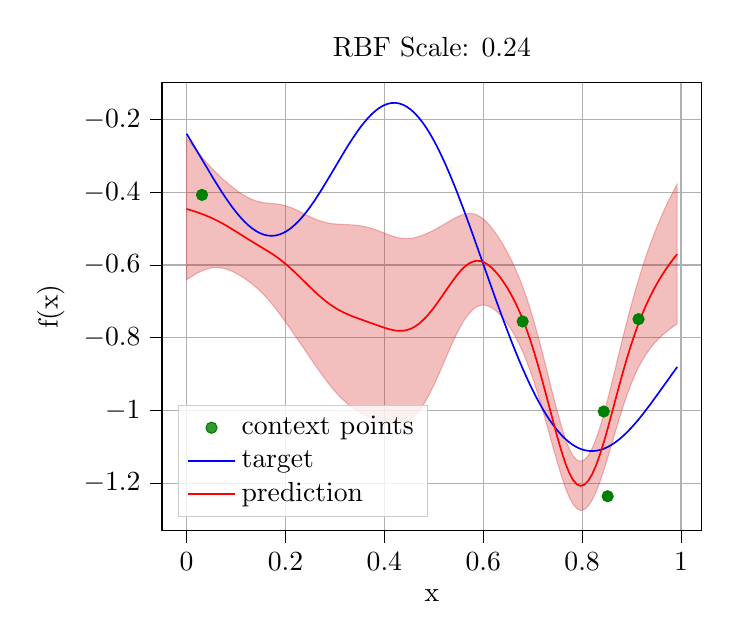
\begin{tikzpicture}

\definecolor{crimson2143940}{RGB}{214,39,40}
\definecolor{darkgray176}{RGB}{176,176,176}
\definecolor{green}{RGB}{0,128,0}
\definecolor{lightgray204}{RGB}{204,204,204}

\begin{axis}[
legend cell align={left},
legend style={
  fill opacity=0.8,
  draw opacity=1,
  text opacity=1,
  at={(0.03,0.03)},
  anchor=south west,
  draw=lightgray204
},
tick align=outside,
tick pos=left,
title={RBF Scale: 0.24},
x grid style={darkgray176},
xlabel={x},
xmajorgrids,
xmin=-0.049609375, xmax=1.041796875,
xtick style={color=black},
y grid style={darkgray176},
ylabel={f(x)},
ymajorgrids,
ymin=-1.33123987838626, ymax=-0.0979588784277439,
ytick style={color=black}
]
\addplot [draw=green, fill=green, mark=*, only marks]
table{%
x  y
0.03125 -0.407177895307541
0.6796875 -0.755326390266418
0.84375 -1.00302398204803
0.8515625 -1.23615598678589
0.9140625 -0.74896651506424
};
\addlegendentry{context points}
\path [draw=crimson2143940, fill=crimson2143940, opacity=0.3]
(axis cs:0,-0.250930607318878)
--(axis cs:0,-0.640730917453766)
--(axis cs:0.0078125,-0.633859992027283)
--(axis cs:0.015625,-0.627196192741394)
--(axis cs:0.0234375,-0.62118262052536)
--(axis cs:0.03125,-0.616000950336456)
--(axis cs:0.0390625,-0.611818730831146)
--(axis cs:0.046875,-0.608944535255432)
--(axis cs:0.0546875,-0.607336521148682)
--(axis cs:0.0625,-0.607151627540588)
--(axis cs:0.0703125,-0.608184814453125)
--(axis cs:0.078125,-0.610496759414673)
--(axis cs:0.0859375,-0.613978207111359)
--(axis cs:0.09375,-0.618479430675507)
--(axis cs:0.1015625,-0.623830258846283)
--(axis cs:0.109375,-0.63003146648407)
--(axis cs:0.1171875,-0.636853158473969)
--(axis cs:0.125,-0.644419312477112)
--(axis cs:0.1328125,-0.652554869651794)
--(axis cs:0.140625,-0.661490797996521)
--(axis cs:0.1484375,-0.671187043190002)
--(axis cs:0.15625,-0.681749701499939)
--(axis cs:0.1640625,-0.693382322788239)
--(axis cs:0.171875,-0.705816626548767)
--(axis cs:0.1796875,-0.719140946865082)
--(axis cs:0.1875,-0.733110666275024)
--(axis cs:0.1953125,-0.747758686542511)
--(axis cs:0.203125,-0.762580931186676)
--(axis cs:0.2109375,-0.777686238288879)
--(axis cs:0.21875,-0.793001651763916)
--(axis cs:0.2265625,-0.808491468429565)
--(axis cs:0.234375,-0.824082791805267)
--(axis cs:0.2421875,-0.83976536989212)
--(axis cs:0.25,-0.855321228504181)
--(axis cs:0.2578125,-0.870914161205292)
--(axis cs:0.265625,-0.886180996894836)
--(axis cs:0.2734375,-0.901079416275024)
--(axis cs:0.28125,-0.915595293045044)
--(axis cs:0.2890625,-0.929402768611908)
--(axis cs:0.296875,-0.942435264587402)
--(axis cs:0.3046875,-0.95461243391037)
--(axis cs:0.3125,-0.965697228908539)
--(axis cs:0.3203125,-0.97586864233017)
--(axis cs:0.328125,-0.984927296638489)
--(axis cs:0.3359375,-0.992944240570068)
--(axis cs:0.34375,-1.00014662742615)
--(axis cs:0.3515625,-1.0063636302948)
--(axis cs:0.359375,-1.01205146312714)
--(axis cs:0.3671875,-1.01695346832275)
--(axis cs:0.375,-1.02153432369232)
--(axis cs:0.3828125,-1.02554488182068)
--(axis cs:0.390625,-1.02914011478424)
--(axis cs:0.3984375,-1.03231000900269)
--(axis cs:0.40625,-1.03489661216736)
--(axis cs:0.4140625,-1.03669393062592)
--(axis cs:0.421875,-1.03751289844513)
--(axis cs:0.4296875,-1.03697884082794)
--(axis cs:0.4375,-1.03487956523895)
--(axis cs:0.4453125,-1.0307332277298)
--(axis cs:0.453125,-1.02428388595581)
--(axis cs:0.4609375,-1.01535272598267)
--(axis cs:0.46875,-1.00370287895203)
--(axis cs:0.4765625,-0.989284038543701)
--(axis cs:0.484375,-0.97213751077652)
--(axis cs:0.4921875,-0.952554225921631)
--(axis cs:0.5,-0.930996060371399)
--(axis cs:0.5078125,-0.907617330551147)
--(axis cs:0.515625,-0.883336961269379)
--(axis cs:0.5234375,-0.858528554439545)
--(axis cs:0.53125,-0.833992958068848)
--(axis cs:0.5390625,-0.810136437416077)
--(axis cs:0.546875,-0.787797391414642)
--(axis cs:0.5546875,-0.767414689064026)
--(axis cs:0.5625,-0.749588787555695)
--(axis cs:0.5703125,-0.734901070594788)
--(axis cs:0.578125,-0.723420202732086)
--(axis cs:0.5859375,-0.715482294559479)
--(axis cs:0.59375,-0.711083948612213)
--(axis cs:0.6015625,-0.710155129432678)
--(axis cs:0.609375,-0.712443351745605)
--(axis cs:0.6171875,-0.717623710632324)
--(axis cs:0.625,-0.725254058837891)
--(axis cs:0.6328125,-0.735010027885437)
--(axis cs:0.640625,-0.746909916400909)
--(axis cs:0.6484375,-0.76075953245163)
--(axis cs:0.65625,-0.776628911495209)
--(axis cs:0.6640625,-0.794695615768433)
--(axis cs:0.671875,-0.815196454524994)
--(axis cs:0.6796875,-0.838164627552032)
--(axis cs:0.6875,-0.863923490047455)
--(axis cs:0.6953125,-0.892471551895142)
--(axis cs:0.703125,-0.923714697360992)
--(axis cs:0.7109375,-0.957194983959198)
--(axis cs:0.71875,-0.992721259593964)
--(axis cs:0.7265625,-1.02975845336914)
--(axis cs:0.734375,-1.06799495220184)
--(axis cs:0.7421875,-1.10629320144653)
--(axis cs:0.75,-1.1437326669693)
--(axis cs:0.7578125,-1.17895996570587)
--(axis cs:0.765625,-1.21084880828857)
--(axis cs:0.7734375,-1.23742973804474)
--(axis cs:0.78125,-1.2574565410614)
--(axis cs:0.7890625,-1.27017939090729)
--(axis cs:0.796875,-1.27518165111542)
--(axis cs:0.8046875,-1.27259004116058)
--(axis cs:0.8125,-1.26275634765625)
--(axis cs:0.8203125,-1.24641215801239)
--(axis cs:0.828125,-1.22415959835052)
--(axis cs:0.8359375,-1.19658672809601)
--(axis cs:0.84375,-1.16521573066711)
--(axis cs:0.8515625,-1.13081729412079)
--(axis cs:0.859375,-1.09487748146057)
--(axis cs:0.8671875,-1.05874645709991)
--(axis cs:0.875,-1.02319896221161)
--(axis cs:0.8828125,-0.989393770694733)
--(axis cs:0.890625,-0.958279430866241)
--(axis cs:0.8984375,-0.929746627807617)
--(axis cs:0.90625,-0.904251635074615)
--(axis cs:0.9140625,-0.881588757038116)
--(axis cs:0.921875,-0.861983895301819)
--(axis cs:0.9296875,-0.844778716564178)
--(axis cs:0.9375,-0.829801440238953)
--(axis cs:0.9453125,-0.816671371459961)
--(axis cs:0.953125,-0.805207371711731)
--(axis cs:0.9609375,-0.794865131378174)
--(axis cs:0.96875,-0.785673022270203)
--(axis cs:0.9765625,-0.777227640151978)
--(axis cs:0.984375,-0.769353568553925)
--(axis cs:0.9921875,-0.762062191963196)
--(axis cs:0.9921875,-0.378130197525024)
--(axis cs:0.9921875,-0.378130197525024)
--(axis cs:0.984375,-0.397635996341705)
--(axis cs:0.9765625,-0.418408632278442)
--(axis cs:0.96875,-0.440363764762878)
--(axis cs:0.9609375,-0.463838934898376)
--(axis cs:0.953125,-0.488938212394714)
--(axis cs:0.9453125,-0.515513181686401)
--(axis cs:0.9375,-0.543933033943176)
--(axis cs:0.9296875,-0.574054539203644)
--(axis cs:0.921875,-0.606221556663513)
--(axis cs:0.9140625,-0.640274941921234)
--(axis cs:0.90625,-0.676502525806427)
--(axis cs:0.8984375,-0.714702486991882)
--(axis cs:0.890625,-0.755001962184906)
--(axis cs:0.8828125,-0.796770036220551)
--(axis cs:0.875,-0.840136528015137)
--(axis cs:0.8671875,-0.884225785732269)
--(axis cs:0.859375,-0.927876234054565)
--(axis cs:0.8515625,-0.970404505729675)
--(axis cs:0.84375,-1.01057267189026)
--(axis cs:0.8359375,-1.04689133167267)
--(axis cs:0.828125,-1.0786749124527)
--(axis cs:0.8203125,-1.10449826717377)
--(axis cs:0.8125,-1.1237518787384)
--(axis cs:0.8046875,-1.13589465618134)
--(axis cs:0.796875,-1.14020526409149)
--(axis cs:0.7890625,-1.13629734516144)
--(axis cs:0.78125,-1.1240086555481)
--(axis cs:0.7734375,-1.10368025302887)
--(axis cs:0.765625,-1.07604169845581)
--(axis cs:0.7578125,-1.0422819852829)
--(axis cs:0.75,-1.00433814525604)
--(axis cs:0.7421875,-0.963415682315826)
--(axis cs:0.734375,-0.920958340167999)
--(axis cs:0.7265625,-0.878139317035675)
--(axis cs:0.71875,-0.836279690265656)
--(axis cs:0.7109375,-0.795972168445587)
--(axis cs:0.703125,-0.757865130901337)
--(axis cs:0.6953125,-0.722171783447266)
--(axis cs:0.6875,-0.689338147640228)
--(axis cs:0.6796875,-0.659409463405609)
--(axis cs:0.671875,-0.632254421710968)
--(axis cs:0.6640625,-0.607474803924561)
--(axis cs:0.65625,-0.584899365901947)
--(axis cs:0.6484375,-0.564298808574677)
--(axis cs:0.640625,-0.545359909534454)
--(axis cs:0.6328125,-0.527886390686035)
--(axis cs:0.625,-0.512099146842957)
--(axis cs:0.6171875,-0.49781060218811)
--(axis cs:0.609375,-0.485319972038269)
--(axis cs:0.6015625,-0.475011557340622)
--(axis cs:0.59375,-0.467062890529633)
--(axis cs:0.5859375,-0.461590826511383)
--(axis cs:0.578125,-0.458748161792755)
--(axis cs:0.5703125,-0.458251565694809)
--(axis cs:0.5625,-0.459850490093231)
--(axis cs:0.5546875,-0.463246494531631)
--(axis cs:0.546875,-0.468038260936737)
--(axis cs:0.5390625,-0.473695188760757)
--(axis cs:0.53125,-0.479872584342957)
--(axis cs:0.5234375,-0.486108243465424)
--(axis cs:0.515625,-0.492361485958099)
--(axis cs:0.5078125,-0.498368978500366)
--(axis cs:0.5,-0.504043102264404)
--(axis cs:0.4921875,-0.509313941001892)
--(axis cs:0.484375,-0.514232099056244)
--(axis cs:0.4765625,-0.518527388572693)
--(axis cs:0.46875,-0.522159576416016)
--(axis cs:0.4609375,-0.524899423122406)
--(axis cs:0.453125,-0.526684880256653)
--(axis cs:0.4453125,-0.527431130409241)
--(axis cs:0.4375,-0.526866674423218)
--(axis cs:0.4296875,-0.525280833244324)
--(axis cs:0.421875,-0.522766709327698)
--(axis cs:0.4140625,-0.51939594745636)
--(axis cs:0.40625,-0.515507698059082)
--(axis cs:0.3984375,-0.511346638202667)
--(axis cs:0.390625,-0.507187604904175)
--(axis cs:0.3828125,-0.503254771232605)
--(axis cs:0.375,-0.499776214361191)
--(axis cs:0.3671875,-0.496675848960876)
--(axis cs:0.359375,-0.494167000055313)
--(axis cs:0.3515625,-0.49219936132431)
--(axis cs:0.34375,-0.490722835063934)
--(axis cs:0.3359375,-0.489744275808334)
--(axis cs:0.328125,-0.489222019910812)
--(axis cs:0.3203125,-0.488706648349762)
--(axis cs:0.3125,-0.488244235515594)
--(axis cs:0.3046875,-0.48769873380661)
--(axis cs:0.296875,-0.486690640449524)
--(axis cs:0.2890625,-0.48519104719162)
--(axis cs:0.28125,-0.483079791069031)
--(axis cs:0.2734375,-0.480152010917664)
--(axis cs:0.265625,-0.47656786441803)
--(axis cs:0.2578125,-0.472314178943634)
--(axis cs:0.25,-0.46744304895401)
--(axis cs:0.2421875,-0.462269604206085)
--(axis cs:0.234375,-0.456869542598724)
--(axis cs:0.2265625,-0.451517224311829)
--(axis cs:0.21875,-0.446468681097031)
--(axis cs:0.2109375,-0.441970109939575)
--(axis cs:0.203125,-0.438278138637543)
--(axis cs:0.1953125,-0.435328543186188)
--(axis cs:0.1875,-0.433210968971252)
--(axis cs:0.1796875,-0.431842029094696)
--(axis cs:0.171875,-0.430903166532516)
--(axis cs:0.1640625,-0.429937541484833)
--(axis cs:0.15625,-0.428580969572067)
--(axis cs:0.1484375,-0.42659604549408)
--(axis cs:0.140625,-0.42373725771904)
--(axis cs:0.1328125,-0.419825077056885)
--(axis cs:0.125,-0.414967656135559)
--(axis cs:0.1171875,-0.409091651439667)
--(axis cs:0.109375,-0.402506738901138)
--(axis cs:0.1015625,-0.395080178976059)
--(axis cs:0.09375,-0.387064039707184)
--(axis cs:0.0859375,-0.378439962863922)
--(axis cs:0.078125,-0.369322419166565)
--(axis cs:0.0703125,-0.359727382659912)
--(axis cs:0.0625,-0.349644422531128)
--(axis cs:0.0546875,-0.338979005813599)
--(axis cs:0.046875,-0.327670931816101)
--(axis cs:0.0390625,-0.315846145153046)
--(axis cs:0.03125,-0.303451001644135)
--(axis cs:0.0234375,-0.290524899959564)
--(axis cs:0.015625,-0.27738082408905)
--(axis cs:0.0078125,-0.264075964689255)
--(axis cs:0,-0.250930607318878)
--cycle;

\addplot [semithick, blue]
table {%
0 -0.238928914070129
0.015625 -0.274168968200684
0.0546875 -0.363261818885803
0.0703125 -0.397175073623657
0.078125 -0.413298010826111
0.0859375 -0.428702235221863
0.09375 -0.443266153335571
0.1015625 -0.456871271133423
0.109375 -0.469402194023132
0.1171875 -0.48075008392334
0.125 -0.490813255310059
0.1328125 -0.499498605728149
0.140625 -0.506723403930664
0.1484375 -0.512415885925293
0.15625 -0.516517162322998
0.1640625 -0.518981575965881
0.171875 -0.519777894020081
0.1796875 -0.518889904022217
0.1875 -0.516316294670105
0.1953125 -0.512071967124939
0.203125 -0.506187677383423
0.2109375 -0.498709440231323
0.21875 -0.489699602127075
0.2265625 -0.479235410690308
0.234375 -0.467408061027527
0.2421875 -0.454323530197144
0.25 -0.440100193023682
0.2578125 -0.424868226051331
0.265625 -0.408768892288208
0.2734375 -0.391952157020569
0.2890625 -0.356808423995972
0.3203125 -0.285237073898315
0.328125 -0.268092751502991
0.3359375 -0.251592636108398
0.34375 -0.235902667045593
0.3515625 -0.221182823181152
0.359375 -0.207585096359253
0.3671875 -0.195252656936646
0.375 -0.184318780899048
0.3828125 -0.17490541934967
0.390625 -0.167122483253479
0.3984375 -0.161066055297852
0.40625 -0.156819701194763
0.4140625 -0.154451966285706
0.421875 -0.154017090797424
0.4296875 -0.155554294586182
0.4375 -0.159087777137756
0.4453125 -0.164627552032471
0.453125 -0.172167778015137
0.4609375 -0.181689739227295
0.46875 -0.193159818649292
0.4765625 -0.206531763076782
0.484375 -0.221746683120728
0.4921875 -0.238733530044556
0.5 -0.257411122322083
0.5078125 -0.277687907218933
0.515625 -0.299463510513306
0.5234375 -0.322629809379578
0.53125 -0.347071409225464
0.5390625 -0.372668266296387
0.546875 -0.39929461479187
0.5625 -0.455116510391235
0.578125 -0.513481259346008
0.6015625 -0.603466510772705
0.625 -0.693280100822449
0.640625 -0.751449465751648
0.65625 -0.807232141494751
0.6640625 -0.83398175239563
0.671875 -0.859850883483887
0.6796875 -0.884757280349731
0.6875 -0.908624887466431
0.6953125 -0.931384563446045
0.703125 -0.952972412109375
0.7109375 -0.973332047462463
0.71875 -0.992412328720093
0.7265625 -1.01016902923584
0.734375 -1.02656364440918
0.7421875 -1.0415632724762
0.75 -1.05514228343964
0.7578125 -1.06727957725525
0.765625 -1.07796061038971
0.7734375 -1.08717620372772
0.78125 -1.09492325782776
0.7890625 -1.10120356082916
0.796875 -1.10602521896362
0.8046875 -1.10940110683441
0.8125 -1.11134994029999
0.8203125 -1.11189615726471
0.828125 -1.11106884479523
0.8359375 -1.10890305042267
0.84375 -1.10543823242188
0.8515625 -1.1007205247879
0.859375 -1.09479975700378
0.8671875 -1.0877320766449
0.875 -1.07957780361176
0.8828125 -1.07040226459503
0.890625 -1.06027555465698
0.8984375 -1.04927217960358
0.90625 -1.03747117519379
0.9140625 -1.0249547958374
0.921875 -1.01180934906006
0.9375 -0.983991622924805
0.953125 -0.954761743545532
0.9921875 -0.880557060241699
};
\addlegendentry{target}
\addplot [semithick, red]
table {%
0 -0.445830821990967
0.015625 -0.452288508415222
0.0234375 -0.455853700637817
0.0390625 -0.463832378387451
0.046875 -0.468307733535767
0.0546875 -0.47315776348114
0.0625 -0.478398084640503
0.0703125 -0.483956098556519
0.078125 -0.489909648895264
0.09375 -0.502771735191345
0.140625 -0.542613983154297
0.1640625 -0.561659932136536
0.171875 -0.568359851837158
0.1796875 -0.575491428375244
0.1875 -0.583160877227783
0.1953125 -0.591543674468994
0.203125 -0.600429534912109
0.2109375 -0.609828233718872
0.2265625 -0.630004405975342
0.2578125 -0.671614170074463
0.265625 -0.681374430656433
0.2734375 -0.690615653991699
0.28125 -0.699337482452393
0.2890625 -0.707296848297119
0.296875 -0.714562892913818
0.3046875 -0.721155643463135
0.3125 -0.726970672607422
0.3203125 -0.732287645339966
0.328125 -0.737074613571167
0.34375 -0.745434761047363
0.375 -0.760655283927917
0.3984375 -0.771828293800354
0.40625 -0.77520215511322
0.4140625 -0.778044939041138
0.421875 -0.780139803886414
0.4296875 -0.781129837036133
0.4375 -0.78087306022644
0.4453125 -0.779082179069519
0.453125 -0.775484323501587
0.4609375 -0.770126104354858
0.46875 -0.762931227684021
0.4765625 -0.753905773162842
0.484375 -0.743184804916382
0.4921875 -0.730934143066406
0.5 -0.717519521713257
0.5078125 -0.702993154525757
0.5234375 -0.672318458557129
0.5390625 -0.641915798187256
0.546875 -0.627917766571045
0.5546875 -0.615330576896667
0.5625 -0.604719638824463
0.5703125 -0.596576333045959
0.578125 -0.591084241867065
0.5859375 -0.588536500930786
0.59375 -0.589073419570923
0.6015625 -0.592583417892456
0.609375 -0.598881721496582
0.6171875 -0.607717156410217
0.625 -0.618676662445068
0.6328125 -0.631448268890381
0.640625 -0.646134853363037
0.6484375 -0.662529230117798
0.65625 -0.680764198303223
0.6640625 -0.701085209846497
0.671875 -0.723725438117981
0.6796875 -0.748787045478821
0.6875 -0.776630878448486
0.6953125 -0.807321667671204
0.703125 -0.840789914131165
0.7109375 -0.876583576202393
0.71875 -0.91450047492981
0.734375 -0.994476675987244
0.75 -1.07403540611267
0.7578125 -1.11062097549438
0.765625 -1.14344525337219
0.7734375 -1.1705549955368
0.78125 -1.19073259830475
0.7890625 -1.20323836803436
0.796875 -1.20769345760345
0.8046875 -1.20424234867096
0.8125 -1.19325411319733
0.8203125 -1.17545521259308
0.828125 -1.15141725540161
0.8359375 -1.12173902988434
0.84375 -1.08789420127869
0.8515625 -1.05061089992523
0.8671875 -0.97148609161377
0.875 -0.931667804718018
0.8828125 -0.893081903457642
0.890625 -0.856640696525574
0.8984375 -0.822224617004395
0.90625 -0.790377140045166
0.9140625 -0.760931849479675
0.921875 -0.734102725982666
0.9296875 -0.709416627883911
0.9375 -0.686867237091064
0.9453125 -0.666092276573181
0.953125 -0.647072792053223
0.9609375 -0.62935209274292
0.96875 -0.613018393516541
0.9765625 -0.59781813621521
0.984375 -0.583494782447815
0.9921875 -0.570096254348755
};
\addlegendentry{prediction}
\end{axis}

\end{tikzpicture}

		% This file was created with matplot2tikz v0.4.0.
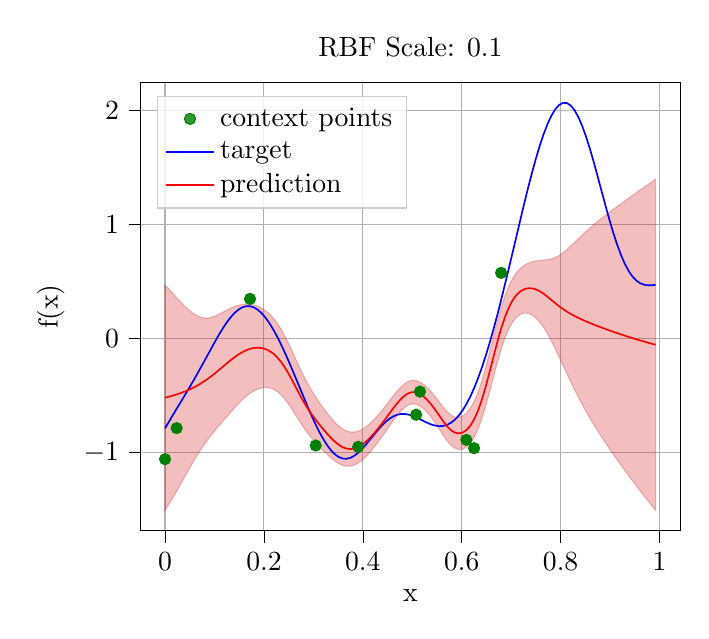
\begin{tikzpicture}

\definecolor{crimson2143940}{RGB}{214,39,40}
\definecolor{darkgray176}{RGB}{176,176,176}
\definecolor{green}{RGB}{0,128,0}
\definecolor{lightgray204}{RGB}{204,204,204}

\begin{axis}[
legend cell align={left},
legend style={
  fill opacity=0.8,
  draw opacity=1,
  text opacity=1,
  at={(0.03,0.97)},
  anchor=north west,
  draw=lightgray204
},
tick align=outside,
tick pos=left,
title={RBF Scale: 0.1},
x grid style={darkgray176},
xlabel={x},
xmajorgrids,
xmin=-0.049609375, xmax=1.041796875,
xtick style={color=black},
y grid style={darkgray176},
ylabel={f(x)},
ymajorgrids,
ymin=-1.68710995316505, ymax=2.24367321133614,
ytick style={color=black}
]
\addplot [draw=green, fill=green, mark=*, only marks]
table{%
x  y
0 -1.05894541740417
0.0234375 -0.786890625953674
0.171875 0.346168965101242
0.3046875 -0.939141511917114
0.390625 -0.950726628303528
0.5078125 -0.669203221797943
0.515625 -0.466711491346359
0.609375 -0.889861762523651
0.625 -0.962745904922485
0.6796875 0.574347078800201
};
\addlegendentry{context points}
\path [draw=crimson2143940, fill=crimson2143940, opacity=0.3]
(axis cs:0,0.466936469078064)
--(axis cs:0,-1.5077155828476)
--(axis cs:0.0078125,-1.45429039001465)
--(axis cs:0.015625,-1.39851355552673)
--(axis cs:0.0234375,-1.34039950370789)
--(axis cs:0.03125,-1.28074407577515)
--(axis cs:0.0390625,-1.21997404098511)
--(axis cs:0.046875,-1.15968155860901)
--(axis cs:0.0546875,-1.1000953912735)
--(axis cs:0.0625,-1.04266059398651)
--(axis cs:0.0703125,-0.988298416137695)
--(axis cs:0.078125,-0.937345683574677)
--(axis cs:0.0859375,-0.890078723430634)
--(axis cs:0.09375,-0.846068561077118)
--(axis cs:0.1015625,-0.804442346096039)
--(axis cs:0.109375,-0.764432489871979)
--(axis cs:0.1171875,-0.725270390510559)
--(axis cs:0.125,-0.685942411422729)
--(axis cs:0.1328125,-0.647220373153687)
--(axis cs:0.140625,-0.609138965606689)
--(axis cs:0.1484375,-0.572738409042358)
--(axis cs:0.15625,-0.538766622543335)
--(axis cs:0.1640625,-0.508454084396362)
--(axis cs:0.171875,-0.482283800840378)
--(axis cs:0.1796875,-0.461010307073593)
--(axis cs:0.1875,-0.444985568523407)
--(axis cs:0.1953125,-0.434858381748199)
--(axis cs:0.203125,-0.43099445104599)
--(axis cs:0.2109375,-0.43435400724411)
--(axis cs:0.21875,-0.445072084665298)
--(axis cs:0.2265625,-0.464781999588013)
--(axis cs:0.234375,-0.493345886468887)
--(axis cs:0.2421875,-0.531016945838928)
--(axis cs:0.25,-0.576609671115875)
--(axis cs:0.2578125,-0.628556728363037)
--(axis cs:0.265625,-0.682785987854004)
--(axis cs:0.2734375,-0.736451089382172)
--(axis cs:0.28125,-0.787149310112)
--(axis cs:0.2890625,-0.833009481430054)
--(axis cs:0.296875,-0.875112473964691)
--(axis cs:0.3046875,-0.913407564163208)
--(axis cs:0.3125,-0.950050175189972)
--(axis cs:0.3203125,-0.984746277332306)
--(axis cs:0.328125,-1.0178142786026)
--(axis cs:0.3359375,-1.04877972602844)
--(axis cs:0.34375,-1.07629132270813)
--(axis cs:0.3515625,-1.09823286533356)
--(axis cs:0.359375,-1.11379098892212)
--(axis cs:0.3671875,-1.12094163894653)
--(axis cs:0.375,-1.11989510059357)
--(axis cs:0.3828125,-1.11036384105682)
--(axis cs:0.390625,-1.09249365329742)
--(axis cs:0.3984375,-1.06777000427246)
--(axis cs:0.40625,-1.03643774986267)
--(axis cs:0.4140625,-0.999989628791809)
--(axis cs:0.421875,-0.95942759513855)
--(axis cs:0.4296875,-0.915365040302277)
--(axis cs:0.4375,-0.868820130825043)
--(axis cs:0.4453125,-0.820839464664459)
--(axis cs:0.453125,-0.771953880786896)
--(axis cs:0.4609375,-0.723901212215424)
--(axis cs:0.46875,-0.678668200969696)
--(axis cs:0.4765625,-0.638667821884155)
--(axis cs:0.484375,-0.606283605098724)
--(axis cs:0.4921875,-0.584081709384918)
--(axis cs:0.5,-0.574225246906281)
--(axis cs:0.5078125,-0.577383100986481)
--(axis cs:0.515625,-0.593112289905548)
--(axis cs:0.5234375,-0.618839800357819)
--(axis cs:0.53125,-0.653621912002563)
--(axis cs:0.5390625,-0.695764601230621)
--(axis cs:0.546875,-0.744167804718018)
--(axis cs:0.5546875,-0.796925187110901)
--(axis cs:0.5625,-0.849908709526062)
--(axis cs:0.5703125,-0.898299336433411)
--(axis cs:0.578125,-0.936954617500305)
--(axis cs:0.5859375,-0.962685942649841)
--(axis cs:0.59375,-0.974236965179443)
--(axis cs:0.6015625,-0.971407473087311)
--(axis cs:0.609375,-0.95343679189682)
--(axis cs:0.6171875,-0.919699370861053)
--(axis cs:0.625,-0.86798620223999)
--(axis cs:0.6328125,-0.796385049819946)
--(axis cs:0.640625,-0.703916490077972)
--(axis cs:0.6484375,-0.593245983123779)
--(axis cs:0.65625,-0.468912541866302)
--(axis cs:0.6640625,-0.339601397514343)
--(axis cs:0.671875,-0.212962821125984)
--(axis cs:0.6796875,-0.0971233695745468)
--(axis cs:0.6875,0.00304484367370605)
--(axis cs:0.6953125,0.0838107913732529)
--(axis cs:0.703125,0.144310757517815)
--(axis cs:0.7109375,0.186380952596664)
--(axis cs:0.71875,0.211371257901192)
--(axis cs:0.7265625,0.221955507993698)
--(axis cs:0.734375,0.219658568501472)
--(axis cs:0.7421875,0.205250307917595)
--(axis cs:0.75,0.179815053939819)
--(axis cs:0.7578125,0.143320083618164)
--(axis cs:0.765625,0.0965725779533386)
--(axis cs:0.7734375,0.0405098795890808)
--(axis cs:0.78125,-0.022766500711441)
--(axis cs:0.7890625,-0.0911297202110291)
--(axis cs:0.796875,-0.163232684135437)
--(axis cs:0.8046875,-0.235990703105927)
--(axis cs:0.8125,-0.308793604373932)
--(axis cs:0.8203125,-0.380035996437073)
--(axis cs:0.828125,-0.448977053165436)
--(axis cs:0.8359375,-0.515420019626617)
--(axis cs:0.84375,-0.579192161560059)
--(axis cs:0.8515625,-0.640487432479858)
--(axis cs:0.859375,-0.699179232120514)
--(axis cs:0.8671875,-0.755874395370483)
--(axis cs:0.875,-0.810374796390533)
--(axis cs:0.8828125,-0.863472044467926)
--(axis cs:0.890625,-0.914956390857697)
--(axis cs:0.8984375,-0.965498089790344)
--(axis cs:0.90625,-1.0147157907486)
--(axis cs:0.9140625,-1.06297731399536)
--(axis cs:0.921875,-1.11029350757599)
--(axis cs:0.9296875,-1.15693938732147)
--(axis cs:0.9375,-1.20290887355804)
--(axis cs:0.9453125,-1.2482727766037)
--(axis cs:0.953125,-1.29299557209015)
--(axis cs:0.9609375,-1.33724105358124)
--(axis cs:0.96875,-1.38080072402954)
--(axis cs:0.9765625,-1.42374575138092)
--(axis cs:0.984375,-1.46619164943695)
--(axis cs:0.9921875,-1.50843799114227)
--(axis cs:0.9921875,1.39648067951202)
--(axis cs:0.9921875,1.39648067951202)
--(axis cs:0.984375,1.37270128726959)
--(axis cs:0.9765625,1.34870302677155)
--(axis cs:0.96875,1.32499694824219)
--(axis cs:0.9609375,1.3012775182724)
--(axis cs:0.953125,1.27720630168915)
--(axis cs:0.9453125,1.25336635112762)
--(axis cs:0.9375,1.22920787334442)
--(axis cs:0.9296875,1.20477879047394)
--(axis cs:0.921875,1.18044149875641)
--(axis cs:0.9140625,1.1559054851532)
--(axis cs:0.90625,1.13085114955902)
--(axis cs:0.8984375,1.10533702373505)
--(axis cs:0.890625,1.07939910888672)
--(axis cs:0.8828125,1.05293726921082)
--(axis cs:0.875,1.02552580833435)
--(axis cs:0.8671875,0.997525691986084)
--(axis cs:0.859375,0.968298494815826)
--(axis cs:0.8515625,0.938216686248779)
--(axis cs:0.84375,0.906777143478394)
--(axis cs:0.8359375,0.874912321567535)
--(axis cs:0.828125,0.842131197452545)
--(axis cs:0.8203125,0.81005585193634)
--(axis cs:0.8125,0.779105007648468)
--(axis cs:0.8046875,0.750905454158783)
--(axis cs:0.796875,0.727161526679993)
--(axis cs:0.7890625,0.70903605222702)
--(axis cs:0.78125,0.696734309196472)
--(axis cs:0.7734375,0.689626753330231)
--(axis cs:0.765625,0.686047375202179)
--(axis cs:0.7578125,0.683353662490845)
--(axis cs:0.75,0.679218769073486)
--(axis cs:0.7421875,0.67181533575058)
--(axis cs:0.734375,0.659730494022369)
--(axis cs:0.7265625,0.641308307647705)
--(axis cs:0.71875,0.614768445491791)
--(axis cs:0.7109375,0.577841639518738)
--(axis cs:0.703125,0.52713531255722)
--(axis cs:0.6953125,0.460148811340332)
--(axis cs:0.6875,0.37404990196228)
--(axis cs:0.6796875,0.268450498580933)
--(axis cs:0.671875,0.146601155400276)
--(axis cs:0.6640625,0.0131790637969971)
--(axis cs:0.65625,-0.123594477772713)
--(axis cs:0.6484375,-0.255783289670944)
--(axis cs:0.640625,-0.374287664890289)
--(axis cs:0.6328125,-0.474637508392334)
--(axis cs:0.625,-0.554044008255005)
--(axis cs:0.6171875,-0.613575279712677)
--(axis cs:0.609375,-0.655154049396515)
--(axis cs:0.6015625,-0.681211173534393)
--(axis cs:0.59375,-0.692360162734985)
--(axis cs:0.5859375,-0.68938934803009)
--(axis cs:0.578125,-0.672417521476746)
--(axis cs:0.5703125,-0.642618536949158)
--(axis cs:0.5625,-0.602903008460999)
--(axis cs:0.5546875,-0.558262944221497)
--(axis cs:0.546875,-0.513214945793152)
--(axis cs:0.5390625,-0.471727550029755)
--(axis cs:0.53125,-0.435463041067123)
--(axis cs:0.5234375,-0.40542083978653)
--(axis cs:0.515625,-0.383187741041183)
--(axis cs:0.5078125,-0.369705975055695)
--(axis cs:0.5,-0.367582619190216)
--(axis cs:0.4921875,-0.377400189638138)
--(axis cs:0.484375,-0.398530781269073)
--(axis cs:0.4765625,-0.428953409194946)
--(axis cs:0.46875,-0.466127455234528)
--(axis cs:0.4609375,-0.507832467556)
--(axis cs:0.453125,-0.551548898220062)
--(axis cs:0.4453125,-0.595349729061127)
--(axis cs:0.4375,-0.637509882450104)
--(axis cs:0.4296875,-0.677495896816254)
--(axis cs:0.421875,-0.714276790618896)
--(axis cs:0.4140625,-0.74694287776947)
--(axis cs:0.40625,-0.774952173233032)
--(axis cs:0.3984375,-0.797391295433044)
--(axis cs:0.390625,-0.812851071357727)
--(axis cs:0.3828125,-0.821119368076324)
--(axis cs:0.375,-0.820952951908112)
--(axis cs:0.3671875,-0.81220668554306)
--(axis cs:0.359375,-0.795085668563843)
--(axis cs:0.3515625,-0.769562602043152)
--(axis cs:0.34375,-0.737409591674805)
--(axis cs:0.3359375,-0.699358224868774)
--(axis cs:0.328125,-0.657275795936584)
--(axis cs:0.3203125,-0.612255752086639)
--(axis cs:0.3125,-0.564669549465179)
--(axis cs:0.3046875,-0.513953924179077)
--(axis cs:0.296875,-0.460283577442169)
--(axis cs:0.2890625,-0.401533484458923)
--(axis cs:0.28125,-0.337914824485779)
--(axis cs:0.2734375,-0.268223106861115)
--(axis cs:0.265625,-0.1946020424366)
--(axis cs:0.2578125,-0.119409412145615)
--(axis cs:0.25,-0.0457594990730286)
--(axis cs:0.2421875,0.0223082602024078)
--(axis cs:0.234375,0.0831661522388458)
--(axis cs:0.2265625,0.135301232337952)
--(axis cs:0.21875,0.179327756166458)
--(axis cs:0.2109375,0.214894235134125)
--(axis cs:0.203125,0.243672072887421)
--(axis cs:0.1953125,0.265632927417755)
--(axis cs:0.1875,0.281938016414642)
--(axis cs:0.1796875,0.292997926473618)
--(axis cs:0.171875,0.298938244581223)
--(axis cs:0.1640625,0.300329953432083)
--(axis cs:0.15625,0.297372728586197)
--(axis cs:0.1484375,0.29031503200531)
--(axis cs:0.140625,0.279639691114426)
--(axis cs:0.1328125,0.265678763389587)
--(axis cs:0.125,0.249249070882797)
--(axis cs:0.1171875,0.230940908193588)
--(axis cs:0.109375,0.212967097759247)
--(axis cs:0.1015625,0.196826159954071)
--(axis cs:0.09375,0.184865891933441)
--(axis cs:0.0859375,0.178531467914581)
--(axis cs:0.078125,0.179237306118011)
--(axis cs:0.0703125,0.187754034996033)
--(axis cs:0.0625,0.203322410583496)
--(axis cs:0.0546875,0.226034045219421)
--(axis cs:0.046875,0.253935694694519)
--(axis cs:0.0390625,0.286325991153717)
--(axis cs:0.03125,0.321286678314209)
--(axis cs:0.0234375,0.357901155948639)
--(axis cs:0.015625,0.394938409328461)
--(axis cs:0.0078125,0.431559860706329)
--(axis cs:0,0.466936469078064)
--cycle;

\addplot [semithick, blue]
table {%
0 -0.788702726364136
0.015625 -0.673458337783813
0.046875 -0.448688268661499
0.0625 -0.331692695617676
0.078125 -0.209595203399658
0.1015625 -0.024061918258667
0.109375 0.0348881483078003
0.1171875 0.0904006958007812
0.125 0.141155004501343
0.1328125 0.185845851898193
0.140625 0.223255753517151
0.1484375 0.252320647239685
0.15625 0.272181749343872
0.1640625 0.282225131988525
0.171875 0.282098770141602
0.1796875 0.271716475486755
0.1875 0.25124192237854
0.1953125 0.221060872077942
0.203125 0.181744575500488
0.2109375 0.134008407592773
0.21875 0.0786707401275635
0.2265625 0.0166175365447998
0.234375 -0.0512244701385498
0.2421875 -0.123905181884766
0.25 -0.200456857681274
0.265625 -0.361185669898987
0.2890625 -0.605267643928528
0.296875 -0.682722330093384
0.3046875 -0.756090641021729
0.3125 -0.82404351234436
0.3203125 -0.885273218154907
0.328125 -0.938543915748596
0.3359375 -0.982757806777954
0.34375 -1.01701760292053
0.3515625 -1.04069375991821
0.359375 -1.05347859859467
0.3671875 -1.05543088912964
0.375 -1.04699885845184
0.3828125 -1.0290242433548
0.390625 -1.00271856784821
0.3984375 -0.969618439674377
0.40625 -0.931516170501709
0.4296875 -0.807043194770813
0.4375 -0.768696546554565
0.4453125 -0.734784960746765
0.453125 -0.706592798233032
0.4609375 -0.685020089149475
0.46875 -0.670546770095825
0.4765625 -0.663221120834351
0.484375 -0.66267728805542
0.4921875 -0.668172359466553
0.5 -0.678644776344299
0.5078125 -0.69278621673584
0.515625 -0.709118366241455
0.5234375 -0.726072311401367
0.53125 -0.742062449455261
0.5390625 -0.755549669265747
0.546875 -0.765093564987183
0.5546875 -0.769389033317566
0.5625 -0.767290115356445
0.5703125 -0.757820010185242
0.578125 -0.740172624588013
0.5859375 -0.713705539703369
0.59375 -0.677931308746338
0.6015625 -0.632504820823669
0.609375 -0.577215433120728
0.6171875 -0.511979341506958
0.625 -0.436836838722229
0.6328125 -0.35195255279541
0.640625 -0.257617712020874
0.6484375 -0.154255151748657
0.65625 -0.0424230098724365
0.6640625 0.0771812200546265
0.671875 0.203720450401306
0.6796875 0.33621871471405
0.6953125 0.614522933959961
0.7265625 1.18571674823761
0.734375 1.32232451438904
0.7421875 1.45296692848206
0.75 1.57579874992371
0.7578125 1.68894648551941
0.765625 1.79053568840027
0.7734375 1.87872815132141
0.78125 1.95176839828491
0.7890625 2.00804471969604
0.796875 2.04615831375122
0.8046875 2.06500124931335
0.8125 2.06384181976318
0.8203125 2.04240250587463
0.828125 2.00093245506287
0.8359375 1.94026112556458
0.84375 1.86182570457458
0.8515625 1.76766502857208
0.859375 1.66037786006927
0.8671875 1.54304111003876
0.8828125 1.29217457771301
0.890625 1.16597652435303
0.8984375 1.04403984546661
0.90625 0.929586887359619
0.9140625 0.825360059738159
0.921875 0.733490109443665
0.9296875 0.655404210090637
0.9375 0.591780066490173
0.9453125 0.542546033859253
0.953125 0.506927490234375
0.9609375 0.48353099822998
0.96875 0.470461845397949
0.9765625 0.465458273887634
0.984375 0.46603798866272
0.9921875 0.469641804695129
};
\addlegendentry{target}
\addplot [semithick, red]
table {%
0 -0.520389556884766
0.0078125 -0.511365294456482
0.015625 -0.501787543296814
0.0234375 -0.491249203681946
0.03125 -0.479728698730469
0.0390625 -0.466824054718018
0.046875 -0.45287299156189
0.0546875 -0.437030673027039
0.0625 -0.419669151306152
0.0703125 -0.400272130966187
0.078125 -0.379054188728333
0.0859375 -0.355773687362671
0.09375 -0.330601334571838
0.1015625 -0.303808093070984
0.1171875 -0.247164726257324
0.125 -0.21834659576416
0.1328125 -0.190770864486694
0.140625 -0.164749622344971
0.1484375 -0.141211748123169
0.15625 -0.120697021484375
0.1640625 -0.104062080383301
0.171875 -0.0916727781295776
0.1796875 -0.0840061902999878
0.1875 -0.0815237760543823
0.1953125 -0.0846127271652222
0.203125 -0.0936611890792847
0.2109375 -0.109729886054993
0.21875 -0.132872104644775
0.2265625 -0.164740324020386
0.234375 -0.205089807510376
0.2421875 -0.254354357719421
0.25 -0.311184644699097
0.2578125 -0.373983144760132
0.2734375 -0.502337098121643
0.28125 -0.562532067298889
0.2890625 -0.617271423339844
0.296875 -0.66769802570343
0.3046875 -0.713680744171143
0.3125 -0.757359862327576
0.3203125 -0.798501014709473
0.328125 -0.837545037269592
0.3359375 -0.874068975448608
0.34375 -0.906850457191467
0.3515625 -0.933897733688354
0.359375 -0.954438328742981
0.3671875 -0.966574192047119
0.375 -0.970423936843872
0.3828125 -0.965741634368896
0.390625 -0.952672362327576
0.3984375 -0.932580709457397
0.40625 -0.905694961547852
0.4140625 -0.87346625328064
0.421875 -0.836852192878723
0.4296875 -0.796430468559265
0.4375 -0.753165006637573
0.453125 -0.661751389503479
0.4609375 -0.615866899490356
0.46875 -0.572397828102112
0.4765625 -0.533810615539551
0.484375 -0.502407193183899
0.4921875 -0.480741024017334
0.5 -0.470903873443604
0.5078125 -0.473544597625732
0.515625 -0.488150000572205
0.5234375 -0.512130260467529
0.53125 -0.544542551040649
0.5390625 -0.583746075630188
0.546875 -0.628691434860229
0.5625 -0.72640585899353
0.5703125 -0.770458936691284
0.578125 -0.804686069488525
0.5859375 -0.826037645339966
0.59375 -0.833298563957214
0.6015625 -0.826309323310852
0.609375 -0.804295420646667
0.6171875 -0.766637325286865
0.625 -0.711015105247498
0.6328125 -0.63551127910614
0.640625 -0.539102077484131
0.6484375 -0.424514651298523
0.65625 -0.296253442764282
0.671875 -0.033180832862854
0.6796875 0.0856635570526123
0.6875 0.188547372817993
0.6953125 0.271979808807373
0.703125 0.335723042488098
0.7109375 0.382111310958862
0.71875 0.413069844245911
0.7265625 0.431631922721863
0.734375 0.43969452381134
0.7421875 0.438532829284668
0.75 0.429516911506653
0.7578125 0.413336873054504
0.765625 0.391309976577759
0.7734375 0.365068316459656
0.7890625 0.308953166007996
0.796875 0.281964421272278
0.8046875 0.257457375526428
0.8125 0.235155701637268
0.8203125 0.215009927749634
0.828125 0.196577072143555
0.8359375 0.179746150970459
0.84375 0.163792490959167
0.8515625 0.14886462688446
0.859375 0.134559631347656
0.8671875 0.1208256483078
0.8828125 0.0947326421737671
0.8984375 0.0699194669723511
0.9140625 0.0464640855789185
0.9296875 0.0239197015762329
0.9453125 0.00254678726196289
0.9609375 -0.0179817676544189
0.9765625 -0.0375213623046875
0.9921875 -0.0559786558151245
};
\addlegendentry{prediction}
\end{axis}

\end{tikzpicture}

	}
	\resizebox{!}{0.40\textheight}{
		% This file was created with matplot2tikz v0.4.0.
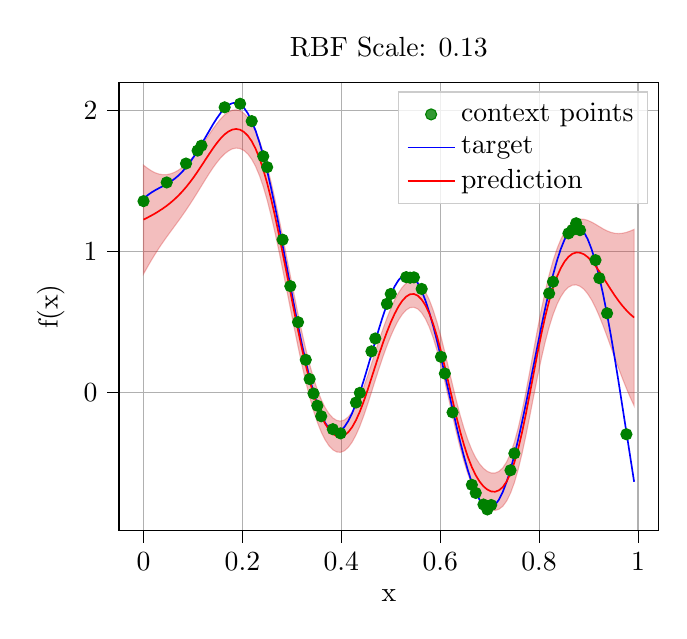
\begin{tikzpicture}

\definecolor{crimson2143940}{RGB}{214,39,40}
\definecolor{darkgray176}{RGB}{176,176,176}
\definecolor{green}{RGB}{0,128,0}
\definecolor{lightgray204}{RGB}{204,204,204}

\begin{axis}[
legend cell align={left},
legend style={fill opacity=0.8, draw opacity=1, text opacity=1, draw=lightgray204},
tick align=outside,
tick pos=left,
title={RBF Scale: 0.13},
x grid style={darkgray176},
xlabel={x},
xmajorgrids,
xmin=-0.049609375, xmax=1.041796875,
xtick style={color=black},
y grid style={darkgray176},
ylabel={f(x)},
ymajorgrids,
ymin=-0.979039061069489, ymax=2.19897757768631,
ytick style={color=black}
]
\addplot [draw=green, fill=green, mark=*, only marks]
table{%
x  y
0 1.35780990123749
0.046875 1.49039375782013
0.0859375 1.62445080280304
0.109375 1.71608781814575
0.1171875 1.75123703479767
0.1640625 2.02289843559265
0.1953125 2.04826211929321
0.21875 1.92503011226654
0.2421875 1.67571794986725
0.25 1.59890413284302
0.28125 1.08466863632202
0.296875 0.755381047725677
0.3125 0.500035345554352
0.328125 0.232932716608047
0.3359375 0.0965583845973015
0.34375 -0.00591184990480542
0.3515625 -0.0922600254416466
0.359375 -0.166812151670456
0.3828125 -0.258695989847183
0.3984375 -0.28831359744072
0.4296875 -0.0698871165513992
0.4375 -0.00119667791295797
0.4609375 0.293070912361145
0.46875 0.384388029575348
0.4921875 0.629891335964203
0.5 0.699996888637543
0.53125 0.819100677967072
0.5390625 0.815229713916779
0.546875 0.817512273788452
0.5625 0.735503971576691
0.6015625 0.254371106624603
0.609375 0.136013701558113
0.625 -0.139365404844284
0.6640625 -0.653137445449829
0.671875 -0.710510075092316
0.6875 -0.792485117912292
0.6953125 -0.827620208263397
0.703125 -0.796193659305573
0.7421875 -0.549833595752716
0.75 -0.430134743452072
0.8203125 0.70395416021347
0.828125 0.786401569843292
0.859375 1.12934052944183
0.8671875 1.15322625637054
0.875 1.20117104053497
0.8828125 1.15223526954651
0.9140625 0.939689874649048
0.921875 0.811904668807983
0.9375 0.563017904758453
0.9765625 -0.294569432735443
};
\addlegendentry{context points}
\path [draw=crimson2143940, fill=crimson2143940, opacity=0.3]
(axis cs:0,1.61297106742859)
--(axis cs:0,0.841336011886597)
--(axis cs:0.0078125,0.890076994895935)
--(axis cs:0.015625,0.937263369560242)
--(axis cs:0.0234375,0.982199311256409)
--(axis cs:0.03125,1.02508199214935)
--(axis cs:0.0390625,1.06552600860596)
--(axis cs:0.046875,1.10414505004883)
--(axis cs:0.0546875,1.14167296886444)
--(axis cs:0.0625,1.17881011962891)
--(axis cs:0.0703125,1.21612334251404)
--(axis cs:0.078125,1.25441288948059)
--(axis cs:0.0859375,1.29385769367218)
--(axis cs:0.09375,1.3350442647934)
--(axis cs:0.1015625,1.37752985954285)
--(axis cs:0.109375,1.42131149768829)
--(axis cs:0.1171875,1.46592104434967)
--(axis cs:0.125,1.51025152206421)
--(axis cs:0.1328125,1.55358600616455)
--(axis cs:0.140625,1.59465181827545)
--(axis cs:0.1484375,1.63221669197083)
--(axis cs:0.15625,1.66550672054291)
--(axis cs:0.1640625,1.69305455684662)
--(axis cs:0.171875,1.71411800384521)
--(axis cs:0.1796875,1.72825992107391)
--(axis cs:0.1875,1.734055519104)
--(axis cs:0.1953125,1.73044085502625)
--(axis cs:0.203125,1.7168310880661)
--(axis cs:0.2109375,1.69213342666626)
--(axis cs:0.21875,1.65519332885742)
--(axis cs:0.2265625,1.60463547706604)
--(axis cs:0.234375,1.53968489170074)
--(axis cs:0.2421875,1.46006989479065)
--(axis cs:0.25,1.36576640605927)
--(axis cs:0.2578125,1.25812745094299)
--(axis cs:0.265625,1.13913214206696)
--(axis cs:0.2734375,1.0113537311554)
--(axis cs:0.28125,0.876637876033783)
--(axis cs:0.2890625,0.738314688205719)
--(axis cs:0.296875,0.599601089954376)
--(axis cs:0.3046875,0.461163103580475)
--(axis cs:0.3125,0.326261907815933)
--(axis cs:0.3203125,0.197675198316574)
--(axis cs:0.328125,0.0778351426124573)
--(axis cs:0.3359375,-0.0304456874728203)
--(axis cs:0.34375,-0.126816973090172)
--(axis cs:0.3515625,-0.209500044584274)
--(axis cs:0.359375,-0.278527528047562)
--(axis cs:0.3671875,-0.334008991718292)
--(axis cs:0.375,-0.37572181224823)
--(axis cs:0.3828125,-0.404477626085281)
--(axis cs:0.390625,-0.419999539852142)
--(axis cs:0.3984375,-0.422624588012695)
--(axis cs:0.40625,-0.411970794200897)
--(axis cs:0.4140625,-0.387707352638245)
--(axis cs:0.421875,-0.350590795278549)
--(axis cs:0.4296875,-0.300012677907944)
--(axis cs:0.4375,-0.237646669149399)
--(axis cs:0.4453125,-0.164368242025375)
--(axis cs:0.453125,-0.0835147649049759)
--(axis cs:0.4609375,0.0026191845536232)
--(axis cs:0.46875,0.0894068852066994)
--(axis cs:0.4765625,0.174653947353363)
--(axis cs:0.484375,0.256037294864655)
--(axis cs:0.4921875,0.331545501947403)
--(axis cs:0.5,0.401030004024506)
--(axis cs:0.5078125,0.46208244562149)
--(axis cs:0.515625,0.514533042907715)
--(axis cs:0.5234375,0.556171596050262)
--(axis cs:0.53125,0.586133539676666)
--(axis cs:0.5390625,0.602993667125702)
--(axis cs:0.546875,0.60539174079895)
--(axis cs:0.5546875,0.593361735343933)
--(axis cs:0.5625,0.565967679023743)
--(axis cs:0.5703125,0.522784292697906)
--(axis cs:0.578125,0.463433027267456)
--(axis cs:0.5859375,0.388121008872986)
--(axis cs:0.59375,0.297360450029373)
--(axis cs:0.6015625,0.192927047610283)
--(axis cs:0.609375,0.0779739618301392)
--(axis cs:0.6171875,-0.0429191365838051)
--(axis cs:0.625,-0.164898797869682)
--(axis cs:0.6328125,-0.283159464597702)
--(axis cs:0.640625,-0.393196284770966)
--(axis cs:0.6484375,-0.491834819316864)
--(axis cs:0.65625,-0.577803492546082)
--(axis cs:0.6640625,-0.650159597396851)
--(axis cs:0.671875,-0.709288656711578)
--(axis cs:0.6796875,-0.755898177623749)
--(axis cs:0.6875,-0.791307747364044)
--(axis cs:0.6953125,-0.816046118736267)
--(axis cs:0.703125,-0.830638468265533)
--(axis cs:0.7109375,-0.834583759307861)
--(axis cs:0.71875,-0.826388359069824)
--(axis cs:0.7265625,-0.805281698703766)
--(axis cs:0.734375,-0.767681479454041)
--(axis cs:0.7421875,-0.712582290172577)
--(axis cs:0.75,-0.63799923658371)
--(axis cs:0.7578125,-0.54314124584198)
--(axis cs:0.765625,-0.430238842964172)
--(axis cs:0.7734375,-0.302185267210007)
--(axis cs:0.78125,-0.165028512477875)
--(axis cs:0.7890625,-0.0241016894578934)
--(axis cs:0.796875,0.113857045769691)
--(axis cs:0.8046875,0.243980526924133)
--(axis cs:0.8125,0.361647248268127)
--(axis cs:0.8203125,0.464757770299911)
--(axis cs:0.828125,0.552304744720459)
--(axis cs:0.8359375,0.623216450214386)
--(axis cs:0.84375,0.679152131080627)
--(axis cs:0.8515625,0.720459699630737)
--(axis cs:0.859375,0.747650861740112)
--(axis cs:0.8671875,0.762145519256592)
--(axis cs:0.875,0.76430881023407)
--(axis cs:0.8828125,0.754480481147766)
--(axis cs:0.890625,0.733311295509338)
--(axis cs:0.8984375,0.700475454330444)
--(axis cs:0.90625,0.657136559486389)
--(axis cs:0.9140625,0.603456676006317)
--(axis cs:0.921875,0.541437268257141)
--(axis cs:0.9296875,0.472495973110199)
--(axis cs:0.9375,0.399192601442337)
--(axis cs:0.9453125,0.323018759489059)
--(axis cs:0.953125,0.24667900800705)
--(axis cs:0.9609375,0.171772003173828)
--(axis cs:0.96875,0.0995835065841675)
--(axis cs:0.9765625,0.0309880971908569)
--(axis cs:0.984375,-0.0331322550773621)
--(axis cs:0.9921875,-0.0929826498031616)
--(axis cs:0.9921875,1.15796875953674)
--(axis cs:0.9921875,1.15796875953674)
--(axis cs:0.984375,1.14597988128662)
--(axis cs:0.9765625,1.13648295402527)
--(axis cs:0.96875,1.13033175468445)
--(axis cs:0.9609375,1.12819588184357)
--(axis cs:0.953125,1.13006567955017)
--(axis cs:0.9453125,1.13652288913727)
--(axis cs:0.9375,1.14706814289093)
--(axis cs:0.9296875,1.16096925735474)
--(axis cs:0.921875,1.17738509178162)
--(axis cs:0.9140625,1.19402813911438)
--(axis cs:0.90625,1.20956897735596)
--(axis cs:0.8984375,1.22181832790375)
--(axis cs:0.890625,1.22936058044434)
--(axis cs:0.8828125,1.23014616966248)
--(axis cs:0.875,1.22316765785217)
--(axis cs:0.8671875,1.20654356479645)
--(axis cs:0.859375,1.17894494533539)
--(axis cs:0.8515625,1.13922274112701)
--(axis cs:0.84375,1.08549642562866)
--(axis cs:0.8359375,1.01732885837555)
--(axis cs:0.828125,0.934151530265808)
--(axis cs:0.8203125,0.834717273712158)
--(axis cs:0.8125,0.719889402389526)
--(axis cs:0.8046875,0.590973615646362)
--(axis cs:0.796875,0.450217366218567)
--(axis cs:0.7890625,0.302192509174347)
--(axis cs:0.78125,0.15192061662674)
--(axis cs:0.7734375,0.00617942214012146)
--(axis cs:0.765625,-0.129668831825256)
--(axis cs:0.7578125,-0.249569818377495)
--(axis cs:0.75,-0.350709021091461)
--(axis cs:0.7421875,-0.430809676647186)
--(axis cs:0.734375,-0.490823745727539)
--(axis cs:0.7265625,-0.53279572725296)
--(axis cs:0.71875,-0.557806491851807)
--(axis cs:0.7109375,-0.569591045379639)
--(axis cs:0.703125,-0.569039285182953)
--(axis cs:0.6953125,-0.557731151580811)
--(axis cs:0.6875,-0.536256611347198)
--(axis cs:0.6796875,-0.504266560077667)
--(axis cs:0.671875,-0.461325705051422)
--(axis cs:0.6640625,-0.406150788068771)
--(axis cs:0.65625,-0.338125973939896)
--(axis cs:0.6484375,-0.256837844848633)
--(axis cs:0.640625,-0.163170754909515)
--(axis cs:0.6328125,-0.0583536848425865)
--(axis cs:0.625,0.0545783489942551)
--(axis cs:0.6171875,0.171302050352097)
--(axis cs:0.609375,0.287089824676514)
--(axis cs:0.6015625,0.397289216518402)
--(axis cs:0.59375,0.497412770986557)
--(axis cs:0.5859375,0.58447003364563)
--(axis cs:0.578125,0.65680730342865)
--(axis cs:0.5703125,0.713901579380035)
--(axis cs:0.5625,0.755632400512695)
--(axis cs:0.5546875,0.782309055328369)
--(axis cs:0.546875,0.794312357902527)
--(axis cs:0.5390625,0.792423903942108)
--(axis cs:0.53125,0.776486456394196)
--(axis cs:0.5234375,0.747699677944183)
--(axis cs:0.515625,0.70733654499054)
--(axis cs:0.5078125,0.656159937381744)
--(axis cs:0.5,0.596318423748016)
--(axis cs:0.4921875,0.527954757213593)
--(axis cs:0.484375,0.453524887561798)
--(axis cs:0.4765625,0.373274028301239)
--(axis cs:0.46875,0.289256304502487)
--(axis cs:0.4609375,0.203909128904343)
--(axis cs:0.453125,0.119514778256416)
--(axis cs:0.4453125,0.0407293736934662)
--(axis cs:0.4375,-0.0301627144217491)
--(axis cs:0.4296875,-0.0898819342255592)
--(axis cs:0.421875,-0.137669116258621)
--(axis cs:0.4140625,-0.171908974647522)
--(axis cs:0.40625,-0.193338930606842)
--(axis cs:0.3984375,-0.201337695121765)
--(axis cs:0.390625,-0.196276247501373)
--(axis cs:0.3828125,-0.178659409284592)
--(axis cs:0.375,-0.14815916121006)
--(axis cs:0.3671875,-0.105048015713692)
--(axis cs:0.359375,-0.0484976470470428)
--(axis cs:0.3515625,0.0212764367461205)
--(axis cs:0.34375,0.104434117674828)
--(axis cs:0.3359375,0.201052308082581)
--(axis cs:0.328125,0.309392035007477)
--(axis cs:0.3203125,0.429193168878555)
--(axis cs:0.3125,0.557717084884644)
--(axis cs:0.3046875,0.692611515522003)
--(axis cs:0.296875,0.83121258020401)
--(axis cs:0.2890625,0.970363676548004)
--(axis cs:0.28125,1.10944962501526)
--(axis cs:0.2734375,1.24537062644958)
--(axis cs:0.265625,1.37478244304657)
--(axis cs:0.2578125,1.49591612815857)
--(axis cs:0.25,1.60617554187775)
--(axis cs:0.2421875,1.70357203483582)
--(axis cs:0.234375,1.7867249250412)
--(axis cs:0.2265625,1.85553288459778)
--(axis cs:0.21875,1.91025018692017)
--(axis cs:0.2109375,1.95147657394409)
--(axis cs:0.203125,1.98041784763336)
--(axis cs:0.1953125,1.99800562858582)
--(axis cs:0.1875,2.00513553619385)
--(axis cs:0.1796875,2.00209927558899)
--(axis cs:0.171875,1.98974943161011)
--(axis cs:0.1640625,1.96950781345367)
--(axis cs:0.15625,1.94198668003082)
--(axis cs:0.1484375,1.90847373008728)
--(axis cs:0.140625,1.87108600139618)
--(axis cs:0.1328125,1.83127355575562)
--(axis cs:0.125,1.79079008102417)
--(axis cs:0.1171875,1.75121343135834)
--(axis cs:0.109375,1.71346175670624)
--(axis cs:0.1015625,1.67862629890442)
--(axis cs:0.09375,1.64734947681427)
--(axis cs:0.0859375,1.61965787410736)
--(axis cs:0.078125,1.59624791145325)
--(axis cs:0.0703125,1.57694983482361)
--(axis cs:0.0625,1.56211042404175)
--(axis cs:0.0546875,1.55169641971588)
--(axis cs:0.046875,1.54604911804199)
--(axis cs:0.0390625,1.54538488388062)
--(axis cs:0.03125,1.54989683628082)
--(axis cs:0.0234375,1.55920970439911)
--(axis cs:0.015625,1.57347691059113)
--(axis cs:0.0078125,1.59178698062897)
--(axis cs:0,1.61297106742859)
--cycle;

\addplot [semithick, blue]
table {%
0 1.37476110458374
0.0078125 1.39869070053101
0.015625 1.4183794260025
0.0234375 1.43502748012543
0.03125 1.44988489151001
0.0390625 1.46420288085938
0.046875 1.47918450832367
0.0546875 1.49593544006348
0.0625 1.51541614532471
0.0703125 1.53839862346649
0.078125 1.56543004512787
0.0859375 1.59679937362671
0.09375 1.63251769542694
0.1015625 1.67230427265167
0.109375 1.71558523178101
0.1171875 1.76150298118591
0.140625 1.90275347232819
0.1484375 1.94590985774994
0.15625 1.98423790931702
0.1640625 2.01594924926758
0.171875 2.03929829597473
0.1796875 2.05264639854431
0.1875 2.05452227592468
0.1953125 2.04367923736572
0.203125 2.0191433429718
0.2109375 1.98025345802307
0.21875 1.92668950557709
0.2265625 1.85849094390869
0.234375 1.77606093883514
0.2421875 1.68016052246094
0.25 1.57189095020294
0.2578125 1.45266652107239
0.265625 1.32417845726013
0.2734375 1.18835115432739
0.2890625 0.903257846832275
0.3046875 0.61557674407959
0.3125 0.476626515388489
0.3203125 0.343979597091675
0.328125 0.219782710075378
0.3359375 0.106022477149963
0.34375 0.0044858455657959
0.3515625 -0.0832743644714355
0.359375 -0.155970931053162
0.3671875 -0.212608575820923
0.375 -0.252506017684937
0.3828125 -0.275312900543213
0.390625 -0.281023025512695
0.3984375 -0.269979119300842
0.40625 -0.242874026298523
0.4140625 -0.200743198394775
0.421875 -0.144951462745667
0.4296875 -0.0771698951721191
0.4375 0.00065147876739502
0.4453125 0.0863239765167236
0.453125 0.177462339401245
0.4765625 0.458011150360107
0.484375 0.545164823532104
0.4921875 0.624897241592407
0.5 0.694877147674561
0.5078125 0.753002882003784
0.515625 0.797458410263062
0.5234375 0.826761245727539
0.53125 0.839805722236633
0.5390625 0.835891723632812
0.546875 0.814745903015137
0.5546875 0.776530742645264
0.5625 0.721840620040894
0.5703125 0.651687145233154
0.578125 0.567473411560059
0.5859375 0.470957398414612
0.59375 0.364206790924072
0.6015625 0.249547004699707
0.6171875 0.00672793388366699
0.6328125 -0.236076354980469
0.640625 -0.350696802139282
0.6484375 -0.457348585128784
0.65625 -0.553652286529541
0.6640625 -0.637456893920898
0.671875 -0.706883788108826
0.6796875 -0.760363578796387
0.6875 -0.796667575836182
0.6953125 -0.814926862716675
0.703125 -0.814647555351257
0.7109375 -0.79571533203125
0.71875 -0.758394002914429
0.7265625 -0.703315019607544
0.734375 -0.63146185874939
0.7421875 -0.544148206710815
0.75 -0.442988872528076
0.7578125 -0.329867839813232
0.765625 -0.206902146339417
0.7734375 -0.0764006376266479
0.7890625 0.197267293930054
0.8046875 0.470468878746033
0.8125 0.600334763526917
0.8203125 0.722311973571777
0.828125 0.83399224281311
0.8359375 0.933129906654358
0.84375 1.01768290996552
0.8515625 1.08584904670715
0.859375 1.13609933853149
0.8671875 1.16720759868622
0.875 1.17827522754669
0.8828125 1.16874980926514
0.890625 1.13843905925751
0.8984375 1.08751726150513
0.90625 1.01652491092682
0.9140625 0.92635977268219
0.921875 0.818261861801147
0.9296875 0.693788170814514
0.9375 0.554781675338745
0.9453125 0.403330445289612
0.953125 0.2417231798172
0.9609375 0.072395920753479
0.9765625 -0.279269456863403
0.9921875 -0.631385326385498
};
\addlegendentry{target}
\addplot [semithick, red]
table {%
0 1.22715353965759
0.0078125 1.24093198776245
0.015625 1.25537014007568
0.0234375 1.27070450782776
0.03125 1.28748941421509
0.0390625 1.30545544624329
0.046875 1.32509708404541
0.0546875 1.34668469429016
0.0625 1.37046027183533
0.0703125 1.39653658866882
0.078125 1.42533040046692
0.0859375 1.45675778388977
0.09375 1.49119687080383
0.1015625 1.52807807922363
0.109375 1.56738662719727
0.125 1.65052080154419
0.1328125 1.69242978096008
0.140625 1.73286890983582
0.1484375 1.77034521102905
0.15625 1.80374670028687
0.1640625 1.83128118515015
0.171875 1.85193371772766
0.1796875 1.86517953872681
0.1875 1.86959552764893
0.1953125 1.86422324180603
0.203125 1.84862446784973
0.2109375 1.82180500030518
0.21875 1.78272175788879
0.2265625 1.73008418083191
0.234375 1.66320490837097
0.2421875 1.58182096481323
0.25 1.48597097396851
0.2578125 1.37702178955078
0.265625 1.25695729255676
0.2734375 1.12836217880249
0.2890625 0.854339122772217
0.3046875 0.576887369155884
0.3125 0.441989421844482
0.3203125 0.31343412399292
0.328125 0.193613529205322
0.3359375 0.0853033065795898
0.34375 -0.0111913681030273
0.3515625 -0.0941118001937866
0.359375 -0.163512587547302
0.3671875 -0.219528436660767
0.375 -0.261940479278564
0.3828125 -0.291568517684937
0.390625 -0.308137893676758
0.3984375 -0.311981201171875
0.40625 -0.30265486240387
0.4140625 -0.279808163642883
0.421875 -0.24412989616394
0.4296875 -0.194947242736816
0.4375 -0.133904695510864
0.4453125 -0.0618194341659546
0.453125 0.0180000066757202
0.4765625 0.273963928222656
0.484375 0.354781150817871
0.4921875 0.429750204086304
0.5 0.498674154281616
0.5078125 0.559121131896973
0.515625 0.610934734344482
0.5234375 0.651935577392578
0.53125 0.681309938430786
0.5390625 0.69770884513855
0.546875 0.699851989746094
0.5546875 0.687835454940796
0.5625 0.660799980163574
0.5703125 0.618342876434326
0.578125 0.560120105743408
0.5859375 0.486295461654663
0.59375 0.39738655090332
0.6015625 0.295108079910278
0.609375 0.182531833648682
0.6328125 -0.170756578445435
0.640625 -0.278183460235596
0.6484375 -0.374336361885071
0.65625 -0.457964777946472
0.6640625 -0.528155207633972
0.671875 -0.585307121276855
0.6796875 -0.630082368850708
0.6875 -0.663782119750977
0.6953125 -0.686888694763184
0.703125 -0.699838876724243
0.7109375 -0.70208740234375
0.71875 -0.692097425460815
0.7265625 -0.669038772583008
0.734375 -0.629252672195435
0.7421875 -0.571696043014526
0.75 -0.494354128837585
0.7578125 -0.396355509757996
0.765625 -0.279953837394714
0.7734375 -0.148002862930298
0.78125 -0.00655388832092285
0.796875 0.282037258148193
0.8046875 0.417477130889893
0.8125 0.540768384933472
0.8203125 0.649737596511841
0.828125 0.743228197097778
0.8359375 0.82027268409729
0.84375 0.88232421875
0.8515625 0.929841279983521
0.859375 0.963297843933105
0.8671875 0.984344482421875
0.875 0.993738174438477
0.8828125 0.992313385009766
0.890625 0.981335878372192
0.8984375 0.961146831512451
0.90625 0.933352708816528
0.9140625 0.898742437362671
0.921875 0.859411239624023
0.9375 0.773130416870117
0.9453125 0.72977089881897
0.953125 0.688372373580933
0.9609375 0.649983882904053
0.96875 0.614957571029663
0.9765625 0.583735466003418
0.984375 0.556423902511597
0.9921875 0.532493114471436
};
\addlegendentry{prediction}
\end{axis}

\end{tikzpicture}

		% This file was created with matplot2tikz v0.4.0.
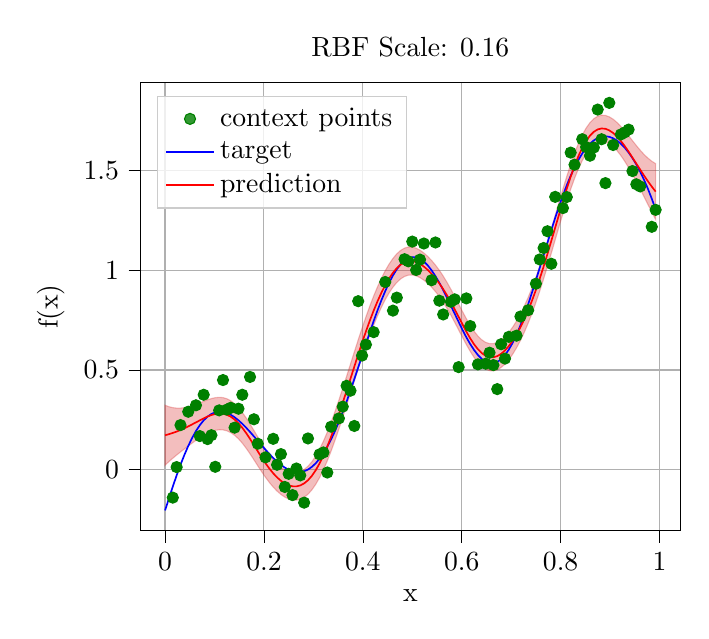
\begin{tikzpicture}

\definecolor{crimson2143940}{RGB}{214,39,40}
\definecolor{darkgray176}{RGB}{176,176,176}
\definecolor{green}{RGB}{0,128,0}
\definecolor{lightgray204}{RGB}{204,204,204}

\begin{axis}[
legend cell align={left},
legend style={
  fill opacity=0.8,
  draw opacity=1,
  text opacity=1,
  at={(0.03,0.97)},
  anchor=north west,
  draw=lightgray204
},
tick align=outside,
tick pos=left,
title={RBF Scale: 0.16},
x grid style={darkgray176},
xlabel={x},
xmajorgrids,
xmin=-0.049609375, xmax=1.041796875,
xtick style={color=black},
y grid style={darkgray176},
ylabel={f(x)},
ymajorgrids,
ymin=-0.307369393110275, ymax=1.94305161833763,
ytick style={color=black}
]
\addplot [draw=green, fill=green, mark=*, only marks]
table{%
x  y
0.015625 -0.140782713890076
0.0234375 0.0124741969630122
0.03125 0.223301634192467
0.046875 0.290305703878403
0.0625 0.322751641273499
0.0703125 0.168172121047974
0.078125 0.375611662864685
0.0859375 0.153029039502144
0.09375 0.172585338354111
0.1015625 0.0139710092917085
0.109375 0.29719278216362
0.1171875 0.449352383613586
0.125 0.30104187130928
0.1328125 0.310201913118362
0.140625 0.210435211658478
0.1484375 0.305497050285339
0.15625 0.375645637512207
0.171875 0.465016812086105
0.1796875 0.252508670091629
0.1875 0.1298718303442
0.203125 0.0613713972270489
0.21875 0.154355853796005
0.2265625 0.0240620393306017
0.234375 0.0776527971029282
0.2421875 -0.087250329554081
0.25 -0.0213457830250263
0.2578125 -0.128125905990601
0.265625 0.00539342686533928
0.2734375 -0.0291735846549273
0.28125 -0.165980145335197
0.2890625 0.15630042552948
0.3125 0.0764417052268982
0.3203125 0.0859965309500694
0.328125 -0.0147307915613055
0.3359375 0.215219244360924
0.3515625 0.256921470165253
0.359375 0.31590062379837
0.3671875 0.420501053333282
0.375 0.395944714546204
0.3828125 0.218961253762245
0.390625 0.845258891582489
0.3984375 0.572290182113647
0.40625 0.627195417881012
0.421875 0.689901649951935
0.4453125 0.941586196422577
0.4609375 0.797937750816345
0.46875 0.863160312175751
0.484375 1.05603492259979
0.4921875 1.04521381855011
0.5 1.14438450336456
0.5078125 1.00189757347107
0.515625 1.05394864082336
0.5234375 1.13475108146667
0.5390625 0.950557947158813
0.546875 1.13994193077087
0.5546875 0.847700536251068
0.5625 0.778648912906647
0.578125 0.842440843582153
0.5859375 0.854452311992645
0.59375 0.514316976070404
0.609375 0.859352290630341
0.6171875 0.720440983772278
0.6328125 0.528135716915131
0.6484375 0.531477034091949
0.65625 0.586675882339478
0.6640625 0.524548232555389
0.671875 0.403894811868668
0.6796875 0.629320204257965
0.6875 0.557079911231995
0.6953125 0.666388988494873
0.7109375 0.672196269035339
0.71875 0.768332600593567
0.734375 0.800018846988678
0.75 0.933004200458527
0.7578125 1.05481159687042
0.765625 1.11214077472687
0.7734375 1.19639194011688
0.78125 1.03309166431427
0.7890625 1.3689421415329
0.8046875 1.31259036064148
0.8125 1.36793231964111
0.8203125 1.59110844135284
0.828125 1.53026258945465
0.84375 1.65839195251465
0.8515625 1.61880052089691
0.859375 1.57554197311401
0.8671875 1.61659646034241
0.875 1.80706143379211
0.8828125 1.65819668769836
0.890625 1.43789076805115
0.8984375 1.84075975418091
0.90625 1.6291788816452
0.921875 1.68228673934937
0.9296875 1.69266092777252
0.9375 1.7065417766571
0.9453125 1.49843001365662
0.953125 1.43219006061554
0.9609375 1.42126441001892
0.984375 1.21854615211487
0.9921875 1.30376839637756
};
\addlegendentry{context points}
\path [draw=crimson2143940, fill=crimson2143940, opacity=0.3]
(axis cs:0,0.322933077812195)
--(axis cs:0,0.0216941684484482)
--(axis cs:0.0078125,0.0398585349321365)
--(axis cs:0.015625,0.0568681359291077)
--(axis cs:0.0234375,0.0729197040200233)
--(axis cs:0.03125,0.0883907675743103)
--(axis cs:0.0390625,0.10344785451889)
--(axis cs:0.046875,0.118173770606518)
--(axis cs:0.0546875,0.132560193538666)
--(axis cs:0.0625,0.146444395184517)
--(axis cs:0.0703125,0.159613281488419)
--(axis cs:0.078125,0.171802878379822)
--(axis cs:0.0859375,0.182492315769196)
--(axis cs:0.09375,0.191118806600571)
--(axis cs:0.1015625,0.197143763303757)
--(axis cs:0.109375,0.19987428188324)
--(axis cs:0.1171875,0.199259579181671)
--(axis cs:0.125,0.194537550210953)
--(axis cs:0.1328125,0.185603022575378)
--(axis cs:0.140625,0.172201439738274)
--(axis cs:0.1484375,0.154316693544388)
--(axis cs:0.15625,0.132626116275787)
--(axis cs:0.1640625,0.107096910476685)
--(axis cs:0.171875,0.0791946649551392)
--(axis cs:0.1796875,0.0493938326835632)
--(axis cs:0.1875,0.0190577954053879)
--(axis cs:0.1953125,-0.0105507075786591)
--(axis cs:0.203125,-0.0387630313634872)
--(axis cs:0.2109375,-0.064655177295208)
--(axis cs:0.21875,-0.0878999605774879)
--(axis cs:0.2265625,-0.108094997704029)
--(axis cs:0.234375,-0.124910540878773)
--(axis cs:0.2421875,-0.138081014156342)
--(axis cs:0.25,-0.147562563419342)
--(axis cs:0.2578125,-0.152811020612717)
--(axis cs:0.265625,-0.153460010886192)
--(axis cs:0.2734375,-0.14909316599369)
--(axis cs:0.28125,-0.139297500252724)
--(axis cs:0.2890625,-0.123723991215229)
--(axis cs:0.296875,-0.10207661986351)
--(axis cs:0.3046875,-0.0743656754493713)
--(axis cs:0.3125,-0.0404715910553932)
--(axis cs:0.3203125,-0.000839486718177795)
--(axis cs:0.328125,0.0439004674553871)
--(axis cs:0.3359375,0.093506321310997)
--(axis cs:0.34375,0.146742433309555)
--(axis cs:0.3515625,0.203184649348259)
--(axis cs:0.359375,0.262140870094299)
--(axis cs:0.3671875,0.32231268286705)
--(axis cs:0.375,0.383164763450623)
--(axis cs:0.3828125,0.444175124168396)
--(axis cs:0.390625,0.504459142684937)
--(axis cs:0.3984375,0.563258290290833)
--(axis cs:0.40625,0.620077192783356)
--(axis cs:0.4140625,0.674043834209442)
--(axis cs:0.421875,0.72469174861908)
--(axis cs:0.4296875,0.771647691726685)
--(axis cs:0.4375,0.81449568271637)
--(axis cs:0.4453125,0.852900862693787)
--(axis cs:0.453125,0.886724650859833)
--(axis cs:0.4609375,0.915639460086823)
--(axis cs:0.46875,0.93919974565506)
--(axis cs:0.4765625,0.957268595695496)
--(axis cs:0.484375,0.96953558921814)
--(axis cs:0.4921875,0.97595226764679)
--(axis cs:0.5,0.976858019828796)
--(axis cs:0.5078125,0.972403228282928)
--(axis cs:0.515625,0.963603854179382)
--(axis cs:0.5234375,0.950779139995575)
--(axis cs:0.53125,0.934753656387329)
--(axis cs:0.5390625,0.915539383888245)
--(axis cs:0.546875,0.893550515174866)
--(axis cs:0.5546875,0.86845725774765)
--(axis cs:0.5625,0.840120553970337)
--(axis cs:0.5703125,0.808868944644928)
--(axis cs:0.578125,0.774738907814026)
--(axis cs:0.5859375,0.738607048988342)
--(axis cs:0.59375,0.701240599155426)
--(axis cs:0.6015625,0.663555145263672)
--(axis cs:0.609375,0.627217054367065)
--(axis cs:0.6171875,0.593374133110046)
--(axis cs:0.625,0.563024938106537)
--(axis cs:0.6328125,0.537693738937378)
--(axis cs:0.640625,0.517834722995758)
--(axis cs:0.6484375,0.504040241241455)
--(axis cs:0.65625,0.496577501296997)
--(axis cs:0.6640625,0.495575785636902)
--(axis cs:0.671875,0.50085312128067)
--(axis cs:0.6796875,0.512355208396912)
--(axis cs:0.6875,0.529403269290924)
--(axis cs:0.6953125,0.551766276359558)
--(axis cs:0.703125,0.579230904579163)
--(axis cs:0.7109375,0.611326932907104)
--(axis cs:0.71875,0.648128092288971)
--(axis cs:0.7265625,0.689276814460754)
--(axis cs:0.734375,0.734904229640961)
--(axis cs:0.7421875,0.784647047519684)
--(axis cs:0.75,0.83856338262558)
--(axis cs:0.7578125,0.896173238754272)
--(axis cs:0.765625,0.957437634468079)
--(axis cs:0.7734375,1.02098953723907)
--(axis cs:0.78125,1.08652901649475)
--(axis cs:0.7890625,1.15330862998962)
--(axis cs:0.796875,1.21974766254425)
--(axis cs:0.8046875,1.28508341312408)
--(axis cs:0.8125,1.34791243076324)
--(axis cs:0.8203125,1.40693283081055)
--(axis cs:0.828125,1.46108388900757)
--(axis cs:0.8359375,1.5093001127243)
--(axis cs:0.84375,1.5506157875061)
--(axis cs:0.8515625,1.58451890945435)
--(axis cs:0.859375,1.61082577705383)
--(axis cs:0.8671875,1.62978100776672)
--(axis cs:0.875,1.64129757881165)
--(axis cs:0.8828125,1.64574790000916)
--(axis cs:0.890625,1.64352071285248)
--(axis cs:0.8984375,1.63485372066498)
--(axis cs:0.90625,1.62049639225006)
--(axis cs:0.9140625,1.60073351860046)
--(axis cs:0.921875,1.57612907886505)
--(axis cs:0.9296875,1.54751396179199)
--(axis cs:0.9375,1.51567876338959)
--(axis cs:0.9453125,1.48103725910187)
--(axis cs:0.953125,1.44491922855377)
--(axis cs:0.9609375,1.4074170589447)
--(axis cs:0.96875,1.3694087266922)
--(axis cs:0.9765625,1.33117532730103)
--(axis cs:0.984375,1.29296278953552)
--(axis cs:0.9921875,1.25516641139984)
--(axis cs:0.9921875,1.53571736812592)
--(axis cs:0.9921875,1.53571736812592)
--(axis cs:0.984375,1.54791283607483)
--(axis cs:0.9765625,1.56342267990112)
--(axis cs:0.96875,1.58198845386505)
--(axis cs:0.9609375,1.60316896438599)
--(axis cs:0.953125,1.62659060955048)
--(axis cs:0.9453125,1.65103662014008)
--(axis cs:0.9375,1.67607057094574)
--(axis cs:0.9296875,1.70012617111206)
--(axis cs:0.921875,1.7225729227066)
--(axis cs:0.9140625,1.74242758750916)
--(axis cs:0.90625,1.75868737697601)
--(axis cs:0.8984375,1.77061140537262)
--(axis cs:0.890625,1.77767622470856)
--(axis cs:0.8828125,1.77884554862976)
--(axis cs:0.875,1.77361631393433)
--(axis cs:0.8671875,1.76134777069092)
--(axis cs:0.859375,1.74153184890747)
--(axis cs:0.8515625,1.71420288085938)
--(axis cs:0.84375,1.67917156219482)
--(axis cs:0.8359375,1.63668167591095)
--(axis cs:0.828125,1.58734822273254)
--(axis cs:0.8203125,1.53214001655579)
--(axis cs:0.8125,1.47223103046417)
--(axis cs:0.8046875,1.40869605541229)
--(axis cs:0.796875,1.34284698963165)
--(axis cs:0.7890625,1.27614760398865)
--(axis cs:0.78125,1.20937585830688)
--(axis cs:0.7734375,1.14413940906525)
--(axis cs:0.765625,1.08122384548187)
--(axis cs:0.7578125,1.0209242105484)
--(axis cs:0.75,0.964600503444672)
--(axis cs:0.7421875,0.912259161472321)
--(axis cs:0.734375,0.864302217960358)
--(axis cs:0.7265625,0.820542454719543)
--(axis cs:0.71875,0.781222283840179)
--(axis cs:0.7109375,0.746068120002747)
--(axis cs:0.703125,0.715322613716125)
--(axis cs:0.6953125,0.688788890838623)
--(axis cs:0.6875,0.666898190975189)
--(axis cs:0.6796875,0.649891138076782)
--(axis cs:0.671875,0.63801497220993)
--(axis cs:0.6640625,0.632050275802612)
--(axis cs:0.65625,0.632128000259399)
--(axis cs:0.6484375,0.638545274734497)
--(axis cs:0.640625,0.651264846324921)
--(axis cs:0.6328125,0.670093178749084)
--(axis cs:0.625,0.694499313831329)
--(axis cs:0.6171875,0.724108695983887)
--(axis cs:0.609375,0.757389545440674)
--(axis cs:0.6015625,0.793396949768066)
--(axis cs:0.59375,0.831000864505768)
--(axis cs:0.5859375,0.868505716323853)
--(axis cs:0.578125,0.904996633529663)
--(axis cs:0.5703125,0.939653217792511)
--(axis cs:0.5625,0.971588492393494)
--(axis cs:0.5546875,1.00072503089905)
--(axis cs:0.546875,1.02672100067139)
--(axis cs:0.5390625,1.04970526695251)
--(axis cs:0.53125,1.07000708580017)
--(axis cs:0.5234375,1.08720147609711)
--(axis cs:0.515625,1.10125601291656)
--(axis cs:0.5078125,1.11130952835083)
--(axis cs:0.5,1.11698567867279)
--(axis cs:0.4921875,1.11721456050873)
--(axis cs:0.484375,1.11181259155273)
--(axis cs:0.4765625,1.10040175914764)
--(axis cs:0.46875,1.08301568031311)
--(axis cs:0.4609375,1.06002628803253)
--(axis cs:0.453125,1.0315682888031)
--(axis cs:0.4453125,0.998133420944214)
--(axis cs:0.4375,0.960091590881348)
--(axis cs:0.4296875,0.917578339576721)
--(axis cs:0.421875,0.870932817459106)
--(axis cs:0.4140625,0.820523917675018)
--(axis cs:0.40625,0.766732037067413)
--(axis cs:0.3984375,0.709992289543152)
--(axis cs:0.390625,0.651187062263489)
--(axis cs:0.3828125,0.590782284736633)
--(axis cs:0.375,0.529563307762146)
--(axis cs:0.3671875,0.468413859605789)
--(axis cs:0.359375,0.407886624336243)
--(axis cs:0.3515625,0.348519384860992)
--(axis cs:0.34375,0.291622519493103)
--(axis cs:0.3359375,0.237886890769005)
--(axis cs:0.328125,0.187743782997131)
--(axis cs:0.3203125,0.142417952418327)
--(axis cs:0.3125,0.102153368294239)
--(axis cs:0.3046875,0.0675596594810486)
--(axis cs:0.296875,0.0391018390655518)
--(axis cs:0.2890625,0.0166653022170067)
--(axis cs:0.28125,0.000308647751808167)
--(axis cs:0.2734375,-0.0102628618478775)
--(axis cs:0.265625,-0.0153135359287262)
--(axis cs:0.2578125,-0.0152201578021049)
--(axis cs:0.25,-0.0103302076458931)
--(axis cs:0.2421875,-0.000947542488574982)
--(axis cs:0.234375,0.0124079361557961)
--(axis cs:0.2265625,0.0297127440571785)
--(axis cs:0.21875,0.0507357195019722)
--(axis cs:0.2109375,0.0751478597521782)
--(axis cs:0.203125,0.102511450648308)
--(axis cs:0.1953125,0.132486641407013)
--(axis cs:0.1875,0.16411118209362)
--(axis cs:0.1796875,0.19666776061058)
--(axis cs:0.171875,0.228811293840408)
--(axis cs:0.1640625,0.259116381406784)
--(axis cs:0.15625,0.286974042654037)
--(axis cs:0.1484375,0.310832977294922)
--(axis cs:0.140625,0.330595672130585)
--(axis cs:0.1328125,0.345534682273865)
--(axis cs:0.125,0.355660170316696)
--(axis cs:0.1171875,0.361283719539642)
--(axis cs:0.109375,0.362710952758789)
--(axis cs:0.1015625,0.360984116792679)
--(axis cs:0.09375,0.356439858675003)
--(axis cs:0.0859375,0.350048243999481)
--(axis cs:0.078125,0.342566251754761)
--(axis cs:0.0703125,0.334760069847107)
--(axis cs:0.0625,0.32728385925293)
--(axis cs:0.0546875,0.320548802614212)
--(axis cs:0.046875,0.314937263727188)
--(axis cs:0.0390625,0.310870677232742)
--(axis cs:0.03125,0.308645874261856)
--(axis cs:0.0234375,0.308583855628967)
--(axis cs:0.015625,0.31084731221199)
--(axis cs:0.0078125,0.315595865249634)
--(axis cs:0,0.322933077812195)
--cycle;

\addplot [semithick, blue]
table {%
0 -0.205077528953552
0.015625 -0.0854612588882446
0.0234375 -0.0290179252624512
0.03125 0.0241776704788208
0.0390625 0.073489785194397
0.046875 0.118387222290039
0.0546875 0.158448100090027
0.0625 0.193363189697266
0.0703125 0.222933530807495
0.078125 0.247067928314209
0.0859375 0.265776634216309
0.09375 0.279163122177124
0.1015625 0.287414908409119
0.109375 0.29079258441925
0.1171875 0.289618492126465
0.125 0.284265160560608
0.1328125 0.275144934654236
0.140625 0.262698769569397
0.1484375 0.247387528419495
0.15625 0.229683041572571
0.1640625 0.210062503814697
0.171875 0.18900191783905
0.1875 0.144443511962891
0.203125 0.0996959209442139
0.2109375 0.0783662796020508
0.21875 0.0583091974258423
0.2265625 0.0399456024169922
0.234375 0.0236865282058716
0.2421875 0.00993156433105469
0.25 -0.000932693481445312
0.2578125 -0.00853729248046875
0.265625 -0.012534499168396
0.2734375 -0.0126035213470459
0.28125 -0.00845754146575928
0.2890625 0.000149250030517578
0.296875 0.0134142637252808
0.3046875 0.0314778089523315
0.3125 0.0544165372848511
0.3203125 0.0822352170944214
0.328125 0.114861488342285
0.3359375 0.152141571044922
0.34375 0.193836569786072
0.3515625 0.239622235298157
0.359375 0.289090037345886
0.3671875 0.341750860214233
0.375 0.397040486335754
0.390625 0.512924909591675
0.4140625 0.689096927642822
0.421875 0.745354175567627
0.4296875 0.79908299446106
0.4375 0.84954047203064
0.4453125 0.896026849746704
0.453125 0.937900066375732
0.4609375 0.974589467048645
0.46875 1.00560748577118
0.4765625 1.03056013584137
0.484375 1.04915428161621
0.4921875 1.06120634078979
0.5 1.06664550304413
0.5078125 1.06551682949066
0.515625 1.05798196792603
0.5234375 1.04431772232056
0.53125 1.02491223812103
0.5390625 1.00026059150696
0.546875 0.970956087112427
0.5546875 0.937681794166565
0.5625 0.901200532913208
0.5703125 0.862339973449707
0.6015625 0.701167941093445
0.609375 0.664103269577026
0.6171875 0.630154848098755
0.625 0.600165247917175
0.6328125 0.574909210205078
0.640625 0.555077791213989
0.6484375 0.541262149810791
0.65625 0.533941745758057
0.6640625 0.53347373008728
0.671875 0.540083169937134
0.6796875 0.55385947227478
0.6875 0.574752807617188
0.6953125 0.602575778961182
0.703125 0.637008666992188
0.7109375 0.677605152130127
0.71875 0.723804950714111
0.7265625 0.774946093559265
0.734375 0.830281734466553
0.7421875 0.88899827003479
0.7578125 1.01309990882874
0.78125 1.20261490345001
0.7890625 1.26327884197235
0.796875 1.32141351699829
0.8046875 1.37636232376099
0.8125 1.4275563955307
0.8203125 1.47452008724213
0.828125 1.51687347888947
0.8359375 1.55433392524719
0.84375 1.586709856987
0.8515625 1.61389589309692
0.859375 1.63586342334747
0.8671875 1.65264868736267
0.875 1.66434049606323
0.8828125 1.6710661649704
0.890625 1.67297780513763
0.8984375 1.67023825645447
0.90625 1.66300654411316
0.9140625 1.65142905712128
0.921875 1.63562655448914
0.9296875 1.61568832397461
0.9375 1.59166574478149
0.9453125 1.56356978416443
0.953125 1.53137040138245
0.9609375 1.49499881267548
0.96875 1.45435214042664
0.9765625 1.40929961204529
0.984375 1.35969078540802
0.9921875 1.30536472797394
};
\addlegendentry{target}
\addplot [semithick, red]
table {%
0 0.172313570976257
0.0078125 0.177727222442627
0.015625 0.183857679367065
0.0234375 0.190751791000366
0.03125 0.1985182762146
0.0390625 0.207159280776978
0.046875 0.21655547618866
0.0625 0.23686408996582
0.078125 0.257184505462646
0.0859375 0.266270279884338
0.09375 0.273779392242432
0.1015625 0.279063940048218
0.109375 0.281292676925659
0.1171875 0.280271649360657
0.125 0.27509880065918
0.1328125 0.265568852424622
0.140625 0.25139856338501
0.1484375 0.232574820518494
0.15625 0.209800124168396
0.1640625 0.183106660842896
0.171875 0.154003024101257
0.1953125 0.0609679222106934
0.203125 0.0318741798400879
0.2109375 0.00524640083312988
0.21875 -0.0185821056365967
0.2265625 -0.0391911268234253
0.234375 -0.0562512874603271
0.2421875 -0.069514274597168
0.25 -0.0789463520050049
0.2578125 -0.0840156078338623
0.265625 -0.0843868255615234
0.2734375 -0.0796780586242676
0.28125 -0.0694944858551025
0.2890625 -0.0535293817520142
0.296875 -0.0314873456954956
0.3046875 -0.0034029483795166
0.3125 0.0308408737182617
0.3203125 0.0707892179489136
0.328125 0.115822076797485
0.3359375 0.165696620941162
0.34375 0.21918249130249
0.3515625 0.275851964950562
0.3671875 0.395363330841064
0.390625 0.577823162078857
0.3984375 0.636625289916992
0.40625 0.693404674530029
0.4140625 0.747283935546875
0.421875 0.797812223434448
0.4296875 0.844613075256348
0.4375 0.887293577194214
0.4453125 0.925517082214355
0.453125 0.959146499633789
0.4609375 0.98783278465271
0.46875 1.01110768318176
0.4765625 1.02883517742157
0.484375 1.04067409038544
0.4921875 1.04658341407776
0.5 1.04692184925079
0.5078125 1.0418564081192
0.515625 1.03242993354797
0.5234375 1.01899027824402
0.53125 1.00238037109375
0.5390625 0.982622385025024
0.546875 0.960135698318481
0.5546875 0.934591054916382
0.5625 0.905854463577271
0.5703125 0.874261140823364
0.578125 0.839867830276489
0.5859375 0.803556442260742
0.609375 0.69230329990387
0.6171875 0.658741474151611
0.625 0.628762125968933
0.6328125 0.603893518447876
0.640625 0.584549784660339
0.6484375 0.571292757987976
0.65625 0.564352750778198
0.6640625 0.563812971115112
0.671875 0.5694340467453
0.6796875 0.581123113632202
0.6875 0.598150730133057
0.6953125 0.620277643203735
0.703125 0.647276759147644
0.7109375 0.67869758605957
0.71875 0.714675188064575
0.7265625 0.754909634590149
0.734375 0.799603223800659
0.7421875 0.848453044891357
0.75 0.901582002639771
0.7578125 0.958548784255981
0.765625 1.01933073997498
0.7734375 1.08256447315216
0.7890625 1.21472811698914
0.8046875 1.34688973426819
0.8125 1.41007173061371
0.8203125 1.46953642368317
0.828125 1.52421605587006
0.8359375 1.57299089431763
0.84375 1.61489367485046
0.8515625 1.64936089515686
0.859375 1.67617881298065
0.8671875 1.69556438922882
0.875 1.70745694637299
0.8828125 1.71229672431946
0.890625 1.71059846878052
0.8984375 1.7027325630188
0.90625 1.68959188461304
0.9140625 1.67158055305481
0.921875 1.64935100078583
0.9296875 1.62382006645203
0.9375 1.59587466716766
0.953125 1.53575491905212
0.96875 1.47569859027863
0.9765625 1.44729900360107
0.984375 1.42043781280518
0.9921875 1.39544188976288
};
\addlegendentry{prediction}
\end{axis}

\end{tikzpicture}

	}
\end{figure}

\section{Conclusion}
\label{exp:conclusion}
